%! TEX root = /home/user/Documents/KTH/notes/SF1625/main.tex
\documentclass{report}

\include{preamble}
\include{macros}
\include{letterfonts}
\usepackage{graphicx}

\graphicspath{{./img/}}
%\usepackage[Glenn]{fncychap}

\usepackage{pgfplots}
\pgfplotsset{width=10cm,compat=1.9}
\usepgfplotslibrary{fillbetween}


\title{\Huge{SF1625 Envariabelanalys}}
\author{\huge{}}
\date{}


\begin{document}

\maketitle
\newpage
\pdfbookmark[section]{\contentsname}{toc}
\tableofcontents
	\pagebreak

\chapter{Modul 1}

\section{Föreläsning 1 (17/01/2023)}
Mängder, intervall, funktioner, grafer \\\\

\subsection{Intervaller}

\nt{ \textbf{Öppet}   intervall: $ (a,b) = \{x : a < x < b\} $ }
\nt{ \textbf{Stängd}  intervall: $ \{x : a \le x \le b\} $ }
\nt{ \textbf{Halvöppet}  intervall: $ (a,b] = \{x : a < x \le b\}$ }

\subsection{Funktioner}

\dfn{Funktion}
{
	En funktion $ f: A \mapsto B $ \textbf{definieras} som en regel att varje element $ x \in A $ associerar \textbf{precis} en element $ f(x) \in B $. Mängden där $ f $ är definierad kallas för \textbf{definitionsmängd} och betecknas som $ D(f),\:D_f $. Mängden av möjliga element $ f(x),\:x \in D_f $ kallas för \textbf{värdemängd} och betecknas som $ R(f),\:R_f $.   
}

\ex{}
{
Funktionen som tar $ x $ och avbildar på $ x^3 $ och är definierad på hela $ \mathbb{R} $ kan vi skriva som $ f(x) = x^3,\:y = x^3,\: x \mapsto x^3 $ 
}

\nt{ \textbf{Konvention:} om definitionsmängden ej anges antas att definitionsmängden är den största \textbf{möjliga} mängd där funktionen är väldefinierad. }

\pagebreak

\ex{ $ f(x) = x^3 $ }
{
1) \textbf{Konventionen} säger att definitionsmängden för $ f(x) $, alltså $ D_f $ är $ \mathbb{R} $.\\\\

2) $ f(x) = \sqrt{x},\:D_f = \{x \in \mathbb{R} :\: \ge 0\} $. Vad är $ R_f $? $ y \in R_f \iff $ det finns $ x \in D_f $ så att $ y = \sqrt{x}  $. Det är bara möjligt om $ y \ge 0 $ och då få får vi $ y^2 = x $. \textbf{Slutsats:} $ R_f = \{y \in \mathbb{R} : y \ge 0\} $\\\\

3) $ g(x) = \frac{1}{x-2} $. Vad är $ D_g $ och $ R_g $? $ D_g = $ alla $ x $ förutom 2 $ \implies D_g = \mathbb{R}\backslash \{2\}$.\\
$ R_g \iff y = \frac{1}{x-2} \iff (y \ne 0)\:x-2 = \frac{1}{y} \iff x = \frac{1}{y}+2 $. \textbf{Alltså:} $ R_g = \mathbb{R}\backslash \{0\} = \{x \in \mathbb{R} : x \ne 0\} $   
}

\subsubsection{Grafer}
I en funktion så måste $ x $ avbilda \textbf{en och endast en} $ y $ värde, annars är \textbf{inte} regeln en funktion. 

\subsubsection{Absolutbelopp}
	\dfn{ $ f(x) = |x| $ }
{
\begin{equation*}
|x| = x,\:x \ge 0\\
\end{equation*}
\begin{equation*}
|x| = -x,\:x<0
\end{equation*}
Är ekvivalent med avståndet från origo. $ |x-a|,\:a \in \mathbb{R} $ tolkas som avståndet från $ x $ till $ a $ och gäller även om $ x < a $ eller $ x > a $.
}

\subsubsection{Udda och jämna funktioner}
\ex{Jämna funktioner $ f(x) = f(-x) $ }
{
	$ 1, x^2, x^4, cos(x) $. Dessa funktioner speglas på $ y $ axeln.  
}

\ex{Udda funktioner $ f(-x) = -f(x) $ }
{
	$ 0, x, x^3, sin(x) $. Dessa funktioner speglas på \textbf{både} $ y $ och $ x $ axeln \textbf{samtidigt}.   
}

\subsubsection{Begränsade funktioner}

\dfn{Begränsade funktioner}
{
Begränsade funktioner definieras som funktioner där det existerar en tal $ M $ sådan att $ |f(x)| \le M $ för alla $ x $ . 
}

\pagebreak
\section{Föreläsning 2 (18/01/2023)}
Gränsvärde, variabelbyte\\

\textbf{Igår:} $ g(x) = \frac{1}{x-2},\:R_g = \mathbb{R} \backslash \{0\} $

\ex{ $ f(x) = \frac{1}{x^2+1}  $ }
{
Finns det något tal $ R $ sådant att $ f(x) < \frac{1}{100}   $ ?\\\\

Vi antar att $ \frac{1}{x^2} < \frac{1}{x^2}  $. Därefter om $ x > 10 $ så får vi $ \frac{1}{x^2}  < \frac{1}{100}  $ och därmed $ \frac{1}{x^2+1} < \frac{1}{100}  $. \textbf{Svar:} Ja, t.ex $ x=10 $.\\\\

Samma fråga för $ 10^{-6} $?\\
\textbf{Svar:} Om $ x > 1000 \implies \frac{1}{x^2+1} < \frac{1}{x^2} < 10^{-6} $. Alltså t.ex $ R=1000 $ är ok.
}

\ex{Avgör om det finns något tal $ \delta $ sådant att $ |x^2+x| < \frac{1}{100}  $ för alla $ x $ sådana $ |x| < \delta $ }
{
		Om $ |x| < 1 $ då gäller $ x^2 < |x| $. Då gäller $ |x^2+x| \le x^2 + |x| \le  2 |x| $.\\
	Därefter om $ |x| < \frac{1}{200}  $ så gäller $ |x^2+x| < 2|x| < \frac{1}{100}  $. \textbf{Svar:} JA, $ \delta = \frac{1}{200}  $ är ok. 
}

\vspace{20pt}
\dfn{Gränsvärdedefinitionen i $ \infty $ }
{
\begin{equation*}
\lim_{x\to \infty} f(x) = L 
\end{equation*}
Om det för varje $ \epsilon > 0 $ finns ett tal $ R $ så att $ |f(x)-L| < \epsilon $ för alla $ x $ sådana att $ x > R $.  
}

\dfn{Gränsdefinitionen i en punkt $ a $ }
{
\begin{equation*}
\lim_{x\to a} f(x) = L 
\end{equation*}
Ekvationen ovan gäller om det för varje $ \epsilon>0 $ finns ett tal $ \delta>0 $ så att $ |f(x)-L| < \epsilon $ för alla $ x $ sådana $ 0 < |x-a| < \delta $. Detta kan omskrivas som vi kan få funktionsvärdena $ f(x) $ hur nära $ L $ som helst bara genom att välja $ x $ tillräckligt nära $ a $. Konceptet illustreras nedan:
\vspace{20pt}
\begin{center}
\includegraphics[scale=0.7]{lim-on-point-a}
\end{center}
}

\vspace{20pt}
\ex{Beräkna $ \lim_{x\to \infty} \frac{1}{x} = 0  $ }
{
	Tag $ \epsilon>0 $, t.ex $ \epsilon> \frac{1}{100} $. Då gäller $ R > 0 $ så att $ x > R \implies \frac{1}{x} < \epsilon \iff x > \frac{1}{ \epsilon} $.\\
	Alltså alla tal $ R $ så att $ R > \frac{1}{ \epsilon}  $ är ok; t.ex välj $ R = \frac{2}{ \epsilon}  $. \textbf{Verifiera:} $ x> \frac{2}{ \epsilon} \iff x < \frac{ \epsilon}{2} $, alltså ok!  
}

Gränsvärderegler om $ f(x)\to L,\:\:g(x)\to M $, då $ x \to a $  :
\begin{itemize}
	\item $ f(x) + g(x) \to L+M $ då $ x\to a $
	\item $ f(x)g(x)\to LM $ då $ x\to a $
	\item $ \frac{f(x)}{g(x)} \to \frac{L}{M}  $ då $ x \to a,\:\: a \ne 0 $
	\item Om $ g(x) \le f(x) \le h(x) $ för $ x $ i en omgivning av $ a $ och dessutom $ g(x) $ och $ h(x) $ har samma gränsvärde när $ x\to a $, så måste även $ f(x) $ ha detta gränsvärde.
\end{itemize}

\pagebreak

\ex{ Bestäm $ \lim_{x\to 1} \frac{x^2-4x+3}{x-1}   $ }
{
$\frac{x^2-4x+3}{x-1} = \frac{(x-1)(x-3)}{(x-1)} $ Alltså $ \lim_{x \to 1} \frac{x^2-4x+3}{x-1} = \lim_{x \to 1} (x-3) = -2 $  
}

\subsubsection{Variabelbyte}

\begin{equation*}
f(x) \to B,\:\:x \to A
\end{equation*}
\begin{equation*}
g(x) \to A,\:\:x \to a
\end{equation*}
$ \implies f(g(x)) \implies y = g(x),\:\:y \to A \implies \lim_{y \to A} f(y) = B$\\
Detta gör att vi kan förenkla många gränsvärdeberäkningar genom variabelbyte.

\ex{Beräkna genom variabelbyte: $ \lim_{x \to 2} (x-3)^2 $ }
{
Anta $ y = x-3 \implies y \to -1$, detta medför $ \lim_{x \to 2} (x-3)^2 \implies \lim_{y \to -1} y^2 = 1$  
}

\vspace{10pt}
\nt{ $ \frac{0}{0} : \lim_{x \to 0} \frac{f(x)}{g(x)}  $ om $ f(x) \to 0 $ och $ g(x) \to 0 $ }
\vspace{10pt}
\ex{Beräkna genom variabelbyte $ \lim_{x \to 1} \frac{sin(x-1)}{x-1}  $ }
{
\begin{equation*}
y = x-1
\end{equation*}
\begin{equation*}
y \to 0
\end{equation*}
\begin{equation*}
\implies \lim_{x \to 1} \frac{sin(x-1)}{x-1} \implies \lim_{y \to 0} \frac{sin(y)}{y} = 1
\end{equation*}
}

\vspace{20pt}
\qs{}
{
\textbf{Bestäm:}
\begin{equation*}
\lim_{t \to 0} \frac{sin(2t)}{t}  
\end{equation*}
}

\sol Anta $ u = 2t $, då $ u \to 0 $. Detta medför att $ \lim_{t \to 0} \frac{sin(2t)}{t} \implies \lim_{u \to 0} \frac{sin(u)}{u} = 1  $  

\vspace{20pt}
\qs{}
{
\textbf{Bestäm:}
\begin{equation*}
\lim_{x \to 1} \frac{x^2-1}{sin(x-1)} 
\end{equation*}
}

\sol Anta $ u = x-1 $, då $ u \to 0 $. Detta medför att $ \lim_{x \to 1} \frac{x^2-1}{sin(x-1)} \implies \frac{u(x+1)}{sin(u)} \iff \frac{x+1}{ \frac{sin(u)}{u} } = \frac{x+1}{1} = 2  $ 

\pagebreak

\dfn{Högergränsvärdet}
{
Om man i gränsvärdesdefinitionen begränsar sig till $ x $ som ligger till höger om $ a $ talar man om högergränsvärdet, skrivet $ \lim_{x \to a^-} f(x) $ 
}

\dfn{Vänstergränsvärdet}
{
Om man i gränsvärdesdefinitionen begränsar sig till $ x $ som ligger till vänster om $ a $ talar man om vänstergränsvärde, skrivet $ \lim_{x \to a^+} f(x) $ 
}

\nt{ \textbf{Krav för gränsvärde:} För att gränsvärdet $ \lim_{x \to a} f(x) $ ska existera, krävs att både \textbf{höger-} och \textbf{vänstergränsvärdena} existerar och \textbf{är} lika.  }
 
\vspace{20pt}
\dfn{Oändliga gränsvärden}
{
Om man kan få $ f(x) $ större än vilket tal som helst bara genom att välja $ x $ tillräckligt nära $ a $ så att 
}

\pagebreak
\section{Föreläsning 3 (19/01/2023)}
Kontinuitet

\dfn{Kontinuitet}
{
Kontinuitet innebär att funktionsvärdet är lika med gränsvärdet i en punkt, det vill säga:
\begin{equation*}
\lim_{x \to a} f(x) = f(a)
\end{equation*}
}

\nt{ Kontinuitet innebär att både höger- och vänstergränsvärde existerar och är lika med funktionsvärdet }

\ex{Diskontinuerlig funktion}
{
Låt funktionen definieras på det sättet:
\begin{equation*}
g(x) = x^2,\:\:x \ne 1
\end{equation*}
\begin{equation*}
g(x) = 2,\:\:x = 1
\end{equation*}

$ g(x) $ är \textbf{diskontinuerlig} i punkten $ x=1 $ 
}

\subsubsection{Kontinuitet i ändpunkter på intervall}
Om en funktion är definierad på ett intervall $ [a,b] $ så säger vi att $ f $ är kontinuerlig i $ a $ om högergränsvärde existerar och sammanfaller med $ f(a) $ (motsvarande för b)

\nt{Alla polynom är kontinuerliga}

\nt{Funktionen $ \frac{1}{x}  $ är också \textbf{kontinuerlig} eftersom vi har \textbf{inte}  definierat värden vid $ x=0 $ }

\vspace{20pt}
\qs{}
{
Bestäm om kontinuerlig:
\begin{equation*}
f(x) = x,\:\: x \le 1
\end{equation*}
\begin{equation*}
	f(x) = x^2+1,\:\: x > 1
\end{equation*}
}
\sol $ \lim_{x \to 1^-} f(x) = 1;\:\: \lim_{x \to 1^+} f(x) = 2;\:\:f(x) = 1   $. \textbf{Slutsats:} ej kontinuerlig 

\vspace{20pt}
\qs{}
{
Bestäm om kontinuerlig
\begin{equation*}
g(x) = \frac{sin(x)}{x},\:\:x > 0
\end{equation*}
\begin{equation*}
g(x) = 1,\:\: x = 0
\end{equation*}
}

\sol $ \lim_{x \to 0^+} g(x) = g(0) = 1 $. \textbf{Slutsats:} Kontinuerlig 

\pagebreak

\noindent
Elementära funktioner är kontinuerliga. Alltså polynom, rationella funktioner, $ x^{ \frac{m}{n} },\:m,n \in \mathbb{Z} $, trigonometriska funktioner, exponentialfunktioner, logaritmer och absolutbeloppet.\\
Kombinationen av kontinuerliga funktioner är också kontinuerliga.\\\\

\thm{Kombination av kontinuerliga funktioner är också kontinuerliga}
{
	Låt $ f: \mathbb{R} \mapsto \mathbb{R} $ och $ g \mathbb{R} \mapsto \mathbb{R} $ vara kontinuerliga på en intervall $ S=[a,b] $. Då gäller följande
\begin{itemize}
	\item $ f+g $ är kontinuerlig på $ S $
	\item $ f-g $ är kontinuerlig på $ S $
	\item $ kf, \: kg $ är kontinuerliga på $ S $ där $ k \in \mathbb{R} $
	\item $ c_1 f+c_2 g $ är också kontinuerlig på $ S $ där $ c_1, c_2 \in \mathbb{R} $ och som kan bevisas med punkt 1 och 3.
	\item $ fg $ är kontinuerlig på $ S $   
	\item $ \frac{f}{g}  $ är kontinuerlig på alla punkter i $ S $ \textbf{där} $ g(x) \ne 0 $ 
\end{itemize}
}

\vspace{20pt}
\noindent
Om $ f $ är \textbf{diskontinuerlig} eller ej definierad i $ a $ och gränsvärdet
\begin{equation*}
\lim_{x \to a} f(x) = L
\end{equation*}
existerar så kan vi definiera en kontinuerlig funktion
\begin{equation*}
	\hat{f}(x) = f(x),\:\:x \ne a
\end{equation*}
\begin{equation*}
	\hat{f}(x) = L,\:\:x = a
\end{equation*}
Detta kallas för \textbf{kontinuerlig utvidgning}. 

\ex{Låt $ f(x) = \frac{x^2-1}{sin(x-1)}  $ }
{
\begin{equation*}
\lim_{x \to 1} \frac{x^2-1}{sin(x-1)} = 2
\end{equation*}
Alltså kan vi definiera den kotninuerliga utvidgningen i $ x=1 $ till $ f $ genom att låta $ f(1) = 2 $.\\\\

\begin{itemize}
	\item $ f $ är kontinuerlig för $ x \ne 1 $ eftersom $ f $ är en kombination av polynom och sinus funktionen.
	\item $ \lim_{x \to 1} f(x) = 2 $ 
\end{itemize} 
En ny funktion $ \hat{f}(x) $ kan då definieras på följande sätt
\begin{equation*}
	\hat{f}(x) = f(x),\:\:x \ne 1
\end{equation*}
\begin{equation*}
	\hat{f}(x) = 2,\:\:x = 1
\end{equation*}
}

\vspace{20pt}
\thm{Max-min satsen}
{
	Om $ f $ är kontinuerlig på ett slutet intervall $ [a,b] $ så antar $ f $ ett största och ett minsta värde på $ [a,b] $ (max och min).
}

\ex{ $ f(x) = \frac{1}{|x-1|},\:f(x) \ge 0 $ och $ \lim_{x \to \infty} f(x) = 0 $ }
{
$ f$ är faktiskt strikt positiv så $ f $ antar ej något min.\\\
$ f $ antar heller inget max.
}

\ex{Vad säger max och min satsen (sats 1.3.1) om följande funktioner?}
{
\begin{equation*}
	f(x) = (x-1)^2,\:x \in [0,1]
\end{equation*}
\begin{equation*}
	g(x) = (x-1)^2,\:x \in (0,1]
\end{equation*}
\begin{equation*}
h(x) = (x-1)^2,\:x \ne 1;\:\:h(x) = 2,\:x = 1 
\end{equation*}
\dotfill\\
1) $ min = 0,\:\:max = 1 $ \\
2) $ min = 0 $ men \textbf{saknar} max\\
3) Falsk exempel\\ 
}

\vspace{20pt}
\thm{Satsen om mellanliggande värde}
{
Om $ f $ är kontinuerlig på ett slutet intervall $ [a,b] $, då antar $ f $ alla värden mellan $ f(a) $ och $ f(b) $.
}

\ex{Visa att ekvationen $ xsin(x)-1 = 0 $ har minst en rot på intervallet $ [0, \frac{\pi}{2}  $ }
{
Kan skrivas om som att bevisa att funktionen $ f(x) = xsin(x)-1 $ är kontinuerlig. Detta görs så eftersom enligt satsen om mellanliggande värde (sats 1.3.2) så gäller att om funktionen $ xsin(x)-1 $ är kontinuerlig så kommer den att passera igenom $ y=0 $, eftersom $ f(0) = -1$ och $ f( \frac{\pi}{2} ) = \frac{\pi}{2}  $ (vänster- och högergränsen av den givna intervallen).  
}

\ex{Med $ f(x) = \frac{1}{x}  $ och intervallet $ [-1,1] $, kan vi inte dra slutsatsen att det finns ett $ x \in (-1,1) $ så att $ f(x)=0 $ ? Varför, varför inte?}
{
	Funktionen $ \frac{1}{x}  $ är kontinuerlig på sin definitionsmängd, men ej på $ [-1,1] $. Därför gäller \textbf{inte} satsen för $ f $ på $ [-1,1] $.
}

\vspace{20pt}
\qs{}
{
Hitta två funktioner $ f,g $ så $ f(x),\:g(x) \to 0 $, då $ x \to 0 $
}

\sol a) T.ex: $ f(x) = 0,\:\:g(x) = x \implies \lim_{x \to 0} \frac{0}{x} = 0  $\\ 
\sol b) T.ex: $ f(x) = -|x|,\:\:g(x) = x^2 \implies \lim_{x \to 0} \frac{-|x|}{x^2} = 0 $\\
\sol c) T.ex: $ f(x) = 3x,\:\:g(x) = x \implies \lim_{x \to 0} \frac{3x}{x} = 3  $\\


\pagebreak
\noindent
Hur kan en funktion vara diskontinuerlig?\\
\begin{itemize}
	\item Gränsvärdet existerar men den \textbf{inte} är lika med funktionsvärdet
	\item Höger- och vänstergränsvärdet existerar men är \textbf{ej} lika
	\item Varken högra- och vänstergränsvärdet existerar
\end{itemize}

\ex{}
{
En sådan funktion som uppfyller 3:e punkten kan beskrivas på följande sätt:
\begin{equation*}
f(x) = 1,\:\:x = 1, \frac{1}{2} , \frac{1}{3} , \ldots
\end{equation*}
\begin{equation*}
f(x) = 0,\:\:x = \text{alla andra punkter} 
\end{equation*}

Det finns punkter godtyckligt $ x=0 $ (tänk $ \frac{1}{k} $ där $ k $ är stort) där $ f $ antar värdet 1. Men $ f(0) = 0 $. Dessutom $ \lim_{x \to 0} f(x) $ existerar ej. $ f $ är \textbf{ej} kontinuerlig i $ x=0 $  
}

\ex{Kan vi definiera $ f_3(x) = sin( \frac{1}{x} ) $ och $ f_4(x) = xsin( \frac{1}{x} ) $ i $ x=0 $ så att de blir kontinuerliga?}
{
Vi vil visa att $ \lim_{x \to 0} x sin( \frac{1}{x} ) = 0 $ och visar då $ \lim_{x \to 0} |xsin( \frac{1}{x} )| = 0 $.\\
Vi vet att $ 0 \le |xsin( \frac{1}{x} )| $ och $ |xsin( \frac{1}{x} )| = |x||sin( \frac{1}{x} )| \le |x| $.\\
\textbf{Alltså:} $ 0 \le |xsin( \frac{1}{x} )| \le |x| $. Då $ \lim_{x \to 0} f_3(x) = 0 $ eftersom $ \lim_{x \to 0} sin( \frac{1}{x} ) = 1 $  
}

\pagebreak
\chapter{Modul 2}
\section{Föreläsning 4 (24/01/2023)}
Derivata, ekvationer för \textbf{tangent- och normallinjen}, deriverbarhet \\\\

\noindent
En \textbf{vertikal} tangent kan definieras på följande sätt för funktionen $ y = f(x) $:
\begin{equation*}
\lim_{h \to 0} \frac{f(a+h)-f(a)}{h} = \pm \infty
\end{equation*}

\dfn{Derivatans definition}
{
Om vi vill bestämma \textbf{lutningen} för funktionen $ f $ i punkten $ a $ så kan vi beräkna gränsvärden som är då lutningen ( \textbf{tangenten} ) i denna punkt:
\begin{equation}
f'(a) = \lim_{h \to 0 } \frac{f(a+h)-f(a)}{h} = k
\end{equation}
För att bestämma \textbf{linjen} som tangerar $ f(a) $ så använder vi formeln nedan:
\begin{equation*}
y = k(x-a) + f(a) \iff f'(a)(x-a)+f(a)
\end{equation*}

Om 1.1 existerar säger vi att funktionen är \textbf{deriverbar} (differentierbar) i $ a $ a.k.a. $ f' $ existerar i $ a $.  
}

\ex{Deriverbarhet av olika funktioner}
{
\begin{itemize}
	\item Funktionen $ f(x) = x^2 $ är deriverbar överallt och derivatan anges nedan:
\begin{equation*}
	f'(a) = \lim_{h \to 0} \frac{(a+h)^2-a^2}{h} = \lim_{h \to 0} \frac{h^2+2ah}{h} = \lim_{h \to 0} h+2a = 2a 
\end{equation*}

	\item Funktionen $ g(x) = |x| $ har derivata $ g'(x) = sgn(x) $ om $ x \ne 0 $:
\begin{equation*}
\lim_{h \to 0} \frac{(a+h)-a}{h},\:\: \text{om}\:\: a > 0,\:\:|h|\:\:\text{litet}  
\end{equation*}
\begin{equation*}
\lim_{h \to 0} \frac{-a-h-(-a)}{h},\:\: \text{om}\:\: a < 0,\:\:|h|\:\: \text{litet}  
\end{equation*}
Vid $ x = 0 $ så existerar \textbf{inte} $ g'(x) $ 
	\item Funktionen som definieras på följande sätt $ h(x) = \sqrt{x},\:x \ge 0;\:\: - \sqrt{-x},\:x < 0 $ har derivatan som beräknas nedan:
\begin{equation*}
h'(0) = \lim_{k \to 0} \frac{h(k)-h(0)}{k} \implies \lim_{k \to 0} \frac{ \sqrt{k} }{k},\: k > 0;\:\: \lim_{k \to 0} \frac{- \sqrt{-k} }{k},\:k < 0 
\end{equation*}
\end{itemize}
}

\qs{}
{
\textbf{Bestäm}: $ f'(0) $ om $ f(x) $:
\begin{equation*}
f(x) = sin(x)
\end{equation*}
}
\sol
\begin{equation*}
	\lim_{h \to 0} \frac{sin(0+h)-sin(0)}{h} \iff \lim_{h \to 0} \frac{sin(h)}{h} + \frac{0}{h} = 1+0 = 1
\end{equation*}

\vspace{20pt}
\qs{}
{
\textbf{Bestäm} $ g'(0) $ om $ g(x) $:
\begin{equation*}
g(x) = x^2,\:x > 0;\:\: g(x) = x^3+x^4,\:x \le 0
\end{equation*}
}

\sol
\begin{equation*}
	g'(0) = \lim_{h \to 0} \frac{g(h)-g(0)}{h} \implies \lim_{h \to 0} \frac{h^2}{h} ,\:h > 0;\:\: \frac{h^3+h^4}{h} ,\: h < 0 \iff g'(0) = 0
\end{equation*}

\vspace{20pt}
\dfn{Höger- och vänsterderivata}
{
\textbf{Högerderivata}:
\begin{equation*}
f_+ ' (a) = \lim_{h \to 0^+} \frac{f(a+h)-f(a)}{h}  
\end{equation*}
\textbf{Vänsterderivata}:
\begin{equation*}
f_-'(a) = \lim_{h \to 0} \frac{f(a+h)-f(a)}{h} 
\end{equation*}
}

\dfn{Deriverbarhet på intervallen $ [a,b] $ }
{
	En funktion $ f $ är deriverbarhet på intervallen $ [a,b] $ om den är deriverbar på intervallen på $ (a,b) $ och det existerar en vänster- och högerderivata på $ a $ respektive $ b $.
}
\nt{Definitionsmängden för $ f',\:D_{f'} $ kan skilja sig från $ D_f $!}

\thm{Om $ f $ är deriverbar i $ a $ så är funktionen $ f $ kontinuerlig i $ a $ }
{ 
\textbf{OBS}: Motsatsen gäller ej!\\\\

\textbf{Bevis}:
\begin{equation*}
\lim_{h \to 0} f(a+h)-f(a) \iff  \frac{f(a+h)-f(a)}{h} h \iff f'(a)h 
\end{equation*}
Alltså gäller $ \lim_{h \to 0} f(a+h)-f(a) = 0 $ eftersom $ \lim_{h \to 0} f'(a)h = 0 $  och vi vet utifrån det att\\$ \lim_{h \to 0} f(a+h) = f(a) \iff  f $ är \textbf{kontinuerlig}. 
}

\vspace{20pt}
\noindent
Kvotregeln:
\begin{equation*}
\frac{d}{dx} \frac{f(x)}{g(x)} = \frac{f'(x)g(x)-f(x)g'(x)}{(g(x))^2},\: g(x) \ne 0 
\end{equation*}
Kedjeregeln:
\begin{equation*}
\frac{d}{dx} f(g(x)) = f'(g(x))g'(x)
\end{equation*}

\ex{Derivera följande funktioner}
{
\begin{itemize}
	\item $ cos(x^4+x^2) = f(g(x)),\:f(x) = cosx,\:g(x) = x^4+x^2;\:\:f'(x) = -sinx,\:g(x) = 4x^3+2x$.\\ \textbf{Alltså}: $ \frac{d}{dx} cos(x^4+x^2) = -sin(x^4+x^2)(4x^3+2x) $
	\item $ \frac{d}{dx} \frac{1}{2x+1} = \frac{d}{dx} (2x+1)^{-1} = f(g(x)) $, där $ f(x) = x^{-1} \iff \frac{1}{x} $ och $ g(x) = 2x+1$. Då gäller följande: $ f'(x) = -\frac{1}{x^2}  $ och $ g'(x) = 2 $.\\ \textbf{Alltså}: $ \frac{d}{dx} \frac{1}{2x+1} = f'(2x+1) \cdot 2 = - \frac{1}{(2x+1)^2} \cdot 2 $     


\end{itemize}
}

\dfn{Normalen i punkten $ (a, f(a)) $ }
{
Om $ f $ är deriverbar i $ a $ så har grafen $ y=f(x) $ en \textbf{normallinje} (inte endast lutning)  i punkten $ (a,f(a)) $ med ekvationen: 
\begin{equation*}
y = f(a) + - \frac{1}{f'(a)} (x-a)
\end{equation*}
\textbf{Normalen} (lutningen) i andra hand beskrivs då som $ - \frac{1}{f'(a)}  $, eftersom = $ - \frac{1}{f'(a)} \cdot f(a) = -1 $ som är då kraven för att två lutningar ska vara \textbf{vinkelrätta}. 
}

\vspace{20pt}
\dfn{Linjär approximation (tangentlinje)}
{
$ f(x) \approx f(a) + f'(a)(x-a) $
}

\ex{Bestäm tangenten och normalen till $ y =x^3 $ i $ x=1 $ }
{
Med $ f(x) =x^3 $ så har vi $ f(1) = 1,\:f'(x) = 3x^2 $. $ f'(1) = 3  $.\\
Då med hjälp av definition 1.4.5 så beskrivs tangentlinjen enligt $ y = 1+3(x-1) $.
\\Normallinjen i andra hand beskrivs med hjälp av definition 1.4.4 som $ y=1- \frac{1}{3} (x-1) $ 
}

\vspace{20pt}
\qs{}
{
\textbf{Derivera}:
\begin{equation*}
	f(x) = \frac{1}{x^2+1} -1 
\end{equation*}
}
\sol
\begin{equation*}
	\frac{1}{x^2+1}-1 = (x^2+1)^{-1}-1;\:\: \frac{d}{dx} \frac{1}{x^2+1} -1 = - \frac{1}{(x^2+1)^2}2x
\end{equation*}

\vspace{20pt}
\qs{}
{
\textbf{Bestäm} en linje som går igenom $ (1,0) $ och tangerar med
\begin{equation*}
y= \frac{1}{x^2+1} -1
\end{equation*}
}
\sol Eftersom $ f(0) = 0 $ och $ f'(0) = 0 $ så är tangentlinjen i $ (0,0) $ parallell med x-axeln. \textbf{Svar}: Linjen $ y=0 $ uppfyller kraven.     

\qs{}
{
Finns det fler än en sådan linje från fråga 9?
}
\sol Om linjen tangerar i $ x=a $ då ges den av:
\begin{equation*}
y = ( \frac{1}{a^2+1} -1)- \frac{2a}{(a^2+1)^2}(x-1) \iff f(a)+f'(a)(x-a) 
\end{equation*}
Och om den passerar genom $ (1,0) $ så gäller följande enligt subtitering:
\begin{equation*}
	0 = ( \frac{1}{a^2+1} -1)- \frac{2a}{(a^2+1)^2}(1-a) 
\end{equation*}
\begin{equation*}
	\implies 2a=a^2-a^4 \iff g(a) = a^4-a^2+2a
\end{equation*}
$ a=0 $ är en lösning. Men $ g(-1) < 0 $ och $ g(-2) > 0 $ och enligt satsen av mellanliggande värden så måste det existera en \textbf{nollrot} i intervallen $ x \in (-2,1) $ och där $ x \ne 0 $.  

\pagebreak

\section{Föreläsning 5 (25/01/2023)}
Fortsättning på derivata. \textbf{Medelvärdesatsen} \\\\

\ex{Bestäm ett närmevärde (approximation) på $ \sqrt{2}  $ genom att använda den linjära approximationen på $ f(x) = \sqrt{x}  $ nära $ x=1 $}
{
Vi använder tangentlinjen i $ x =1$ för att approximera $ f(2) = \sqrt{2}  $.
\begin{equation*}
\sqrt{2} = f(2) \approx f(1)+(2-1)f'(1)\:\:\:(a=1,\:\:x=2) 
\end{equation*}
Vi har $ f(1) = 1 $ , $ f'(x) = \frac{1}{2} \frac{1}{ \sqrt{x} }  $ och $ f'(1) = \frac{1}{2}  $. Då får vi att
\begin{equation*}
\sqrt{2} \approx 1 + \frac{1}{2} = \frac{3}{2} 
\end{equation*}

}

\vspace{20pt}
\thm{Om $ f $ är definierad på ett öppet intervall $ (a,b) $ och antar sitt maximum eller minimum i en punkt $ c $ i $ (a,b) $ och $ f'(c) $ existerar, så är $ f'(c) = 0 $ }
{
\textbf{Notera}: Punkter där $ f' = 0 $ kallas \textbf{kritiska} eller \textbf{stationära} punkter.\\\\

max/min $ \implies  $ \textbf{kritisk punkt}. \textbf{Notera}: relationen är \textbf{inte} ekvivalent.\\
Det existerar också \textbf{undantag}  som till exempel med $ g(x) = |x-a| $ eftersom $ g'(a) $ är \textbf{inte} definierat.\\\\ 

\textbf{Bevis}: Antar att $ f $ har max i $ c $. Vi vet att $ f'(c) = f_\pm'(c) $. (Samma vänster- och högergränsvärde)
\begin{equation*}
f_+'(c) = \lim_{h \to 0^+} \frac{f(c+h)-f(c)}{h} \le 0
\end{equation*}
\begin{equation*}
f_-'(c) \ge 0
\end{equation*}
Då måste $ f'(c) = 0 $ eftersom det är endast $ f'(c) = 0 $ som uppfyller ekvationen $ 0 \le f'(c) \le 0 $.
}


\pagebreak
\thm{ \textbf{Medelvärdesatsen} }
{
	Om $ f $ är kontinuerlig på $ [a,b] $ och deriverbar på $ (a,b) $ så finns det en punkt $ c \in (a,b) $ sådan att:
\begin{equation*}
f'(c) = \frac{f(b)-f(a)}{b-a} 
\end{equation*}
\dotfill\\
\textbf{Med andra ord}:\\
	Låt en funktion $ f $ vara definierad och kontinuerlig i intervallen $ [a,b] $ då måste \textbf{sekanten} mellan punkterna $  (a, f(a)) $  och $(b, f(b)) $ ha samma lutning som $ f'(c) $, där $ c $ är någon punkt i intervallen $ [a,b] $. Se bilden nedan:   
\begin{center}
		\includegraphics[scale=0.2]{mean_value_theoreum}
\end{center}
}

\vspace{20pt}
\ex{}
{
\textbf{Medelvärdesatsen} innebär t.ex att om du har sprungit 10km på en timme så har du vid någon tidspunkt hållt hastigheten 10km/h
}

\ex{Bevisa att $ f(x) = |x| $ är \textbf{ej} deriverbar i vissa punkter}
{
	Vi vet att $ |x| $ är definierad i intervallen $ [-1,1] $. Då medför medelvärdesatsen att \textbf{sekanten} mellan $ (-1,f(-1)) $ och $ (1,f(1)) $ ha samma lutning som $ f'(c) $ för någon punkt i intervallen $ [-1,1] $. Sekanten mellan $ (-1,f(-1)) $ och $ (1,f(1)) $ har lutningen 0, men vi vet att $ f'(x) $ inte har en sådan derivata. Detta medför att derivatan av $ f $ måste ha en punkt som \textbf{inte} är deriverbar.
}

\ex{Visa att $ \sqrt{1+x} \le 1+ \frac{x}{2} $ för $ x > 0 $ (Typiskt tentatal) }
{
\textbf{OBS}: Medelvärdesatsen säger med $ f(x) = \sqrt{x}  $ :
\begin{equation*}
f(x+1)-f(1) = f'(c)x,\:\:c \in (1,1+x) \iff f(x+1) = f(1) +xf'(c)
\end{equation*}
	$ f $ och $ f' $ kan skrivas om enligt dess definition för att få följande om $ f'(x) = - \frac{1}{2 \sqrt{x} }  $ :
\begin{equation*}
\sqrt{x+1} = 1 + x \frac{1}{2} \frac{1}{ \sqrt{c} } \le 1 + \frac{x}{2} 
\end{equation*}
Vi vet också att $ c > 1 \implies \frac{1}{ \sqrt{c} } \le 1 $.\\
\textbf{V.S.B} 
}

\qs{}
{
\textbf{Visa} att ekvationen (typisk tentatal)
\begin{equation*}
f(x) = 4x^5+x^3+7x-2=0
\end{equation*}
Har exakt \textbf{en} lösning. \textbf{Tips}: Satsen om mellanliggande värde ger existens av en lösning. Använd sedan medelvärdesatsen och anta att det finns minst två lösningar.
}
\sol $ f(-1) < 0 $ och $ f(1) > 0 \implies f$ måste gå igenom $ y=0 $ enligt satsen om mellanligande värde.\\
Vi \textbf{antar} att det existerar 2 \textbf{nollrötter}, då måste det existera en \textbf{sekant} så att dess lutning är 0. Men\\
$ f'(x) = 20x^4+3x^2+7 $ som är \textbf{alltid} positiv för alla $ x \in \mathbb{R} $. Alltså $ f'(x) $ kan \textbf{aldrig} passera genom $ f'(x) = 0 $ som medför en \textbf{motsägelse} om att det existerar fler än en nollrötter i $ \mathbb{R} $.     

\vspace{30pt}
\ex{Funktionen $ f(x) = x^3 $ är strängt växande för alla $ x \in \mathbb{R} $ }
{
\begin{equation*}
f(x) > 0,\:\: \forall x \in \mathbb{R},\:x \ne 0
\end{equation*}
$ f $ är till och med strängt växande trots att $ f'(0) = 0 $ 
}

\ex{Funktionen $ g(x) = \sqrt{x(2-x)}  $ är strängt växande på $ [0,1] $ och strängt avtagande på $ [1,2] $. (D.v.s. för kontinuerliga funktioner sprider sig växandet/avtagandet till intervallets ändpunkter}
{
\begin{equation*}
f'(x) = \frac{1}{2} \frac{1}{ \sqrt{x(2-x)} } (2-2x)
\end{equation*}
Utifrån det kan vi dra slutsatsen att det är $ 2-2x $ som avgör tecknet på $ f' $.
\begin{itemize}
	\item $ f' > 0 $, om $ x < 1 $
	\item $ f' < 0 $, om x $ x > 1 $
	\item $ f'(1) = 0 $ 
\end{itemize}
\textbf{Alltså}: $ f $ är växande om $ x \le 1 $ och $ f $ är avtagande om $ x \ge 1 $.
}
\pagebreak

\section{Föreläsning 6 (26/01/2023)}
Repetition från föreläsning 5 om derivata och medelvärdesatsen + implicit derivering
\ex{Avgör om $ f(x) = x^3-3x^2+1 $ antar ett största och minsta värde när $ x $ varierar i intervallet $ [-1,3] $. Bestäm största och minsta värdet om de finns.}
{
1)\\
$ f $ är kontinuerlig (p.g.a. polynom) på $ [-1,3] $. Max/min $ \implies f $ antar max och min på $ [-1,3] $.\\\\

2)\\
$ f' $ är definierad överallt $ \implies  $ max/min antas i vändpunkter eller kritiska punkter. Max/min värde är \textbf{nollrötterna} till derivatan $ f'(x) = 3x^2-6x $. $ f'(x) = 0 \implies x_1 = 0,\:\: x_2 = 2 $. För att bestämma om $ x_1 $ och $ x_2 $ är max/min punkter så tar man \textbf{närliggande} punkter som är lätt att beräkna och använder för att beräkna luttningen i dessa punkter. Om en punkt åt vänster till $ x_1 = 0 $ har en positiv lutning så innebär det att $ x_1=0 $ är en max punkt. En negativ lutning implicerar motsatsen (min punkt).\\\\
\begin{equation}
f'(-1) > 0;\:\:f'(1) = < 0;\:\:f'(3) = > 0
\end{equation}
Utifrån 2.2 så kan vi se att $ x_1 = 0 $ är en max punkt och $ x_2 = 2 $ är en min punkt.  
}

\vspace{20pt}
\qs{}
{
1. Derivera:
\begin{equation*}
f(x) = x^2 sin( \frac{1}{x} ),\:\:x \ne 0
\end{equation*}
\begin{equation*}
f(x) = 0,\:\:x = 0
\end{equation*}

2. Vad är definitionsmängden för $ f' $?\\
3. Är $ f' $ kontinuerlig där?
}

\sol\\
1.
\begin{equation*}
f'(x) = 2xsin( \frac{1}{x} ) + x^2cos( \frac{1}{x} ) \cdot -\frac{1}{x^2},\:\:x \ne 0
\end{equation*}
\begin{equation*}
f'(x) = 0,\:\:x = 0
\end{equation*}
2. Definitionsmängden för $ f' $ är $ \forall x \in \mathbb{R}$.\\
3. Kan \textbf{inte} vara kontinuerlig eftersom:
\begin{equation*}
\lim_{x \to 0} sin( \frac{1}{x} ) = sin( \infty)
\end{equation*}
konvergerar \textbf{inte}. 

\pagebreak
\qs{}
{
Låt $ f(x) = (x-3)^4(-x^2+6x-6) $. Visa med hjälp av medelvärdesatsen att det \textbf{finns} någon punkt där derivatan försvinner. (Blir 0)\\
\textbf{Tips}: Använd medelvärdesatsen på $ [2,4] $
}
\sol
\begin{equation*}
f'(x) = 4(x-3)^3(-x^2+6x-6)+(-2x+6)(x-3)^4
\end{equation*}
För att beräkna medelvärdesatsen så börjar vi med att beräkna gränsvärden för tips-intervallen vi fick.\\
$f(2) = 2,\:\:f(4) = 2$. Detta innebär att $ f'(c) = 0 $ för någon $ c \in [2,4] $. Vi vet att $ f'(2) = -6 $ och $ f'(4) = 6 $ och vi vet att derivatan, $ f' $ \textbf{är} kontinuerlig alltså enligt satsen om mellanliggande värden så kan vi dra slutsatsen att $ f'(c) = 0 $ för någon $ c \in [2,4] $.\textbf{V.S.B} 

\vspace{30pt}
\subsection{Implicit derivering}
\textbf{Kedjeregeln} säger följande:
\begin{equation*}
\frac{d}{dx}f(g(x)) = f'(g(x))g'(x)
\end{equation*}
Genom att utnyttja kedjeregeln så kan vi hitta derivator och tangentlinje för \textbf{kurvor} (inte funktioner), som t.ex för cirkelns ekvation (kurva) $ x^2+y^2=r^2 $. Detta kallas för \textbf{implicit derivering} när funktionen $ y $ är blandad med $ x $ termer. 

\ex{Hitta lutningen för tangenten i punkten $ ( \frac{1}{2} , \frac{ \sqrt{3} }{2}   $ på cirkeln $ x^2+y^2 = 1 $  }
{
	Genom att derivera cirkelns ekvation med \textbf{implicit deriviering} så får man följande:
\begin{equation*}
\frac{d}{dx} x^2+y^2 = 1 \implies \frac{d}{dx} x^2 + \frac{d}{dx} y^2 = \frac{d}{dx}1 \iff 2x+2y \frac{dy}{dx} = 0
\end{equation*}
Vi kan isolera $ \frac{dy}{dx} $ från ekvationen ovan så att $ y' = \frac{-x}{y}  $. Med $ x = \frac{1}{2}  $ och $ y = \frac{ \sqrt{3} }{2} $ får vi $ y'( \frac{1}{2} ) = - \frac{1}{ \sqrt{3} }  $ i punkten $ ( \frac{1}{2}, \frac{ \sqrt{3} }{2} )$. \textbf{Svar}: lutningen i cirkeln genom origo och med radius 1, i punkten $ ( \frac{1}{2}, \frac{ \sqrt{3} }{2} ) $ är $ - \frac{1}{ \sqrt{3} }  $.    
}

\ex{Bestäm derivatan $ y= \frac{1}{}  $ med hjälp av \textbf{implicit} deriviering}
{
\begin{equation*}
y = \frac{1}{x} \iff xy = 1
\end{equation*}
\begin{equation*}
\frac{d}{dx} xy = 1 \iff \frac{d}{dx} xy = \frac{d}{dx} 1 \iff y+xy' = 0
\end{equation*}
Genom att isolera $ y' $ från ekvationen ovan så får vi följande:
\begin{equation*}
y' = - \frac{y}{x} = - \frac{1}{x^2} 
\end{equation*}
}

\pagebreak
\qs{}
{
En kurvan ges av ekvationen
\begin{equation*}
x^4 + y^4 +xy = 1
\end{equation*}
Bestäm kurvans skärningspunkter med x-axeln. Bestäm tangentens lutning i dessa punkter. 
}

\sol x-axeln = $ y=0 $. Ersätning av ekvationen med $ y=0 $ ger följande: 
\begin{equation*}
x^4+0^4+x \cdot 0 = 1
\end{equation*}
För $ \mathbb{R} $ så har ekvationen $ x^4 = 1 $ endast \textbf{2} lösningar, $ x_1 = 1 $ och $ x_2 = -1 $. Genom att använda implicit derivering så blir derivatan av ekvationen följande:
\begin{equation*}
\frac{d}{dx} x^4 + y^4 + xy = 1 \iff 4x^3 + 4y^3 \frac{dy}{dx} + y + x \frac{dy}{dx} = 0
\end{equation*}
Derivatan av ekvationen kan isoleras från ekvationen ovan för att få:
\begin{equation*}
y' = \frac{-4x^3-y}{4y^3+x} 
\end{equation*}
Genom att använda $ y = 0 $ (för vårt fall) så blir derivatan $ y' = \frac{-4x^3}{x} = -4x^2  $. Genom att sätta $ x_1 = 1 $ så får vi att dess lutning är $ y'(1) = -4 $. För $ x_2 = -1 $ så blir lutningen $ y'(-1) = -4 $.  

\vspace{50pt}
\nt{ \textbf{DE}: Är synonym med \textbf{differentialekvation} som är en ekvation som innehåller en eller flera derivator av en funktion som obekanta. En lösning är helt enkelt en funktion vars derivator uppfyller ekvationen. Lösningar är i många fall \textbf{inte} unika utan kan modifieras med \textbf{konstanter} }

\nt{ \textbf{IVP}: Ett \textbf{begynnelsevärdesproblem} (initialvärdesproblem) är en \textbf{DE} tillsammans med att funktionens värde (och evt derivators värde) är givna i någon punkt  }

\pagebreak

\chapter{Modul 3}

\section{Föreläsning 7 (30/01/2023)}
Transcedenta funktioner, invers, exponentialfunktioner, logaritmfunktioner, potens- och log-lagar.\\\\

\dfn{Injektiva funktioner}
{
En funktion är en regel som till varje tal i definitionsmängden ordnar ett bestämt tal i värdemängden.\\\\

\textbf{Injektiva funktioner} avbildar olika $ x $ på olika $ y $, dvs:
\begin{equation*}
x_1 \ne x_2 \implies f(x_1) \ne f(x_2)
\end{equation*}
Ett annat sätt att säga exakt samma sak är:
\begin{equation*}
f(x_1) = f(x_2) \implies x_1 = x_2
\end{equation*}
Såna funktioner kalla alltså \textbf{injektiva} eller \textbf{ett-till-ett}. 
}

\ex{ $ sin(x) $ är \textbf{ej} injektiv eftersom $ sin(x+2 \pi n) = sin(x) $ }
{
}

\vspace{20pt}
\dfn{Invers}
{
För \textbf{injektiva}  funktioner går det alltså (i princip) att för alla funtionsvärden $ y = f(x) $ tala om precis vilket $ x $ de kom ifrån.\\\\

\textbf{Ex}: Om $ y=f(x) = 2x+1 $, så måste $ x = \frac{y-1}{2} $. Detta ger oss en ny funktion som kallas \textbf{inversen} till $ f $ och kan skrivs som $ f^{-1} $. I vårt exempel så är inversen, $ f^{-1}(y) = \frac{y-1}{2}  $.\\\\

I allmänheten kan man för injektiva $ f $ definiera inversen på samma sätt genom:
\begin{equation*}
	f^{-1}(y) = x \iff y = f(x)
\end{equation*}

Det innebär att vi löser ekvationen $ y=f(x) $ där $ x $ blir en funktion av $ y $.\\\\


En inverterbar fnktion och dess invers uppfyller alltid:
\begin{equation*}
	f^{-1}(f(x)) = x, \forall x \in D_f
\end{equation*}
\begin{equation*}
	f(f^{-1}(y)) = y, \forall y \in D_{f^{-1}}
\end{equation*}
}

\nt{Definitionsmängden för $ f $ är \textbf{värdemängden} för $ f^{-1} $ }
\nt{Strängt växande och strängt avtagande funktioner \textbf{alltid} är injektiva och alltså \textbf{inverterbara} }

\nt{ $ f^{-1} \ne \frac{1}{f}  $. Dock kedjeregeln ger $ \frac{df^{-1}}{dx}  = \frac{1}{f'(f^{-1}(x))} $ som kan bevisas med hjälp av kedjeregeln.
\begin{equation*}
	y = f(f^{-1}(y)),\:\:y' = f'(f^{-1}(y)) \cdot (f^{-1})'(y) = 1 \iff (f^{-1})'(y) = \frac{1}{f'(f^{-1}(y))}  
\end{equation*}
}

\nt{ $ D_{f^{-1}} = V_f = R_f $ }

\vspace{20pt}
\noindent
Minns att variabelnamnet är valfritt, men ofta vill man ha $ x $ som variabelbyte i funktionen, även för inversen. Det är smidigt när man ritar grafen i xy-planet t.ex att man får det som man är van vid.\\\\

\noindent
Om man byter $ y $ mot $ x $ så motsvarar det geometriskt en spegling i linjen $ y=x $.

\ex{}
{
\begin{itemize}
	\item $ f(x) = x^2 $
	\item $ g(x) = x^2, x \ge 0 $
	\item $ h(x) = x |x| $ 
\end{itemize}
}

\dfn{ $ f $ är strängt växande/avtagande}
{
	Om $ f $ är strängt växande, så gäller följande:
	\begin{equation*}
	x_1 > x_0 \implies f(x_1) > f(x_0),\:\: \forall x_1,x_0 \in D_f
	\end{equation*}
	Om $ f $ är strängt avtagande, så gäller följande:
	\begin{equation*}
	x_1 < x_0 \implies f(x_1) < f(x_0),\:\: \forall x_1,x_0 \in D_f
	\end{equation*}
}

\vspace{20pt}
\qs{}
{
Bestäm inversen till funktionen $ f $ som ges av:
\begin{equation*}
f(x) = x^2 + 1,\:\: x \le 0
\end{equation*}
Ange inversens definitionsmängd och värdemängd.
}
\sol $ D_{f^{-1}} = V_f = R_f = x \ge 1 $. $ V_{f^{-1}} = R_{f^{-1}} = D_f = x \le 0 $
\begin{equation*}
	f^{-1}(x) \implies y = x^2+1 \iff y-1 = x^2 \implies f^{-1}(x) = -\sqrt{x-1}   
\end{equation*}

\vspace{20pt}
\qs{}
{
	Visa att $ g(x) = x^5+x^3+1 $ är inverterbar. Kan du bestämma $ (g^{-1})'(3) $? Kan du bestämma $ g^{-1}(x) $?
}
\sol Vi vet att om en funktion är strängt växande eller strängt avtagande så är den inverterbar. Vi kan se om funktionen är strängt växande eller avtagande genom att analysera dess derivata.
\begin{equation*}
y' = 5x^4+3x^2
\end{equation*}
Eftersom $ y' $ består av $ kx^n$, där $ n $ är jämn heltal, så kommer $ V_{y'} = R_{y'} = y \ge 0, \forall x \in \mathbb{R}$. Alltså dess derivata är alltid positiv och \textbf{därmed} originella funktionen, $ y $ är strikt positiv och \textbf{därmed} injektiv och \textbf{inverterbar}.\\\\

\noindent
\textbf{Hittar}: $ (g^{-1})'(3) $:\\
Eftersom $ g(1) = 3 \iff g^{-1}(3) = 1 $. Då om man använder formeln:
\begin{equation*}
	(g^{-1})' = \frac{1}{g'(g^{-1}(x))} 
\end{equation*}
Detta ger att $ (g^{-1})'(3) = \frac{1}{g'(1)} = \frac{1}{8}  $ 

\pagebreak
\dfn{Exponentialfunktionen}
{
\begin{equation*}
y = exp(x) = e^x
\end{equation*}
Den har en derivata:
\begin{equation*}
\frac{d}{dx}e^x = e^x
\end{equation*}
Den är strängt växande på hela reela axeln
}

\dfn{Logaritmfunktionen}
{
Eftersom exponentialfuntkionen är strängt växande är den injektiv och därmed har invers. Inversen kallas för \textbf{naturliga logalgoritmen}, $ y=ln(x) $.\\\\

Dess derivata är
\begin{equation*}
\frac{d}{dx}ln(x) = \frac{1}{x} 
\end{equation*}

Logaritmlagarna är följande:
\begin{itemize}
	\item $ ln(st) = ln(s) + ln(t) $
	\item $ ln( \frac{s}{t} ) = ln(s) - ln(t) $
	\item $ ln(s^t) = t ln(s) $
	\item $ ln(1) = 0 $
	\item $ ln(e^x) = x, \forall x \iff e^{ln(x)} x, x \ge 0$
	\item $ ln \frac{1}{x} = - lnx $ 
\end{itemize}
}

\vspace{20pt}
\qs{}
{
Förenkla följande:
\begin{equation*}
	ln \frac{1}{e},\:\:\: 2lnx+ln \frac{3}{x^2},\:\:\: ln(e^{ln(x)}) 
\end{equation*}
}
\sol\\
1)\\
\begin{equation*}
	ln \frac{1}{e} \iff ln(e^{-1}) = -1
\end{equation*}
2)\\
\begin{equation*}
2lnx+ln \frac{3}{x^2} \iff lnx^2 + ln \frac{3}{x^2} \iff ln(x^2 \frac{3}{x^2} ) = ln(3)   
\end{equation*}
3)\\
\begin{equation*}
	ln(e^{ln(x)}) \iff  ln(x) ln(e) = ln(x) 
\end{equation*}
\pagebreak

\qs{}
{
Bestäm inversen till funktionen $ h $ som ges av
\begin{equation*}
	h(x) = 2e^{3x} + 1
\end{equation*}
och ange inversens definitionsmängd och värdemängd.
}
	\sol $ D_{f^{-1}} = V_f = R_f = y > 1 $. $ V_{f^{-1}} = D_f = x \in (- \infty, \infty)$  
\begin{equation*}
	y = 2e^{3x}+1 \iff \frac{y-1}{2} = e^{3x} \implies \frac{ln( \frac{y-1}{2} )}{3} =x
\end{equation*}

\vspace{30pt}
\ex{Sant eller falskt: Om en funktion är strängt växande så är dess invers strängt avtagande?}
{
Falskt, ex: $ f(x) = x,\:\: f'(x) = 1 $.
}

\pagebreak
\section{Föreläsning 8 (1/02/2023)}
Gränsvärden och arcusfunktioner.\\\\

\noindent
Att deriviera $ f(x)^{g(x)} $ kan göras genom att skriva om den till $ e^{g(x)ln(f(x)) } $ och sedan tillämpa kedjeregeln.

\ex{Deriviera $ x^x $ }
{
	$ x^x $ kan skrivas om till $ (e^{lnx})^x = e^{xlnx} = f(g(x)) $ där $ f(x) = e^x $ och $ g(x) = xlnx $.
\begin{equation*}
	\frac{d}{dx} x^x = f'(g(x)) \cdot g'(x) = e^{xlnx} \cdot (lnx+1) \iff x^x(lnx+1)
\end{equation*}
}

\ex{Bestäm gränsvärde utan L'Hopitals regel}
{
\textbf{Bestäm}:
\begin{equation*}
	\lim_{x \to 0} \frac{e^x-1}{x}  
\end{equation*}
Detta är derivatan av funktionen $ e^x $ i punkten $ x=0 $, som det kan ses nedan:
\begin{equation*}
	\lim_{x \to 0} \frac{e^{x+0}-e^0}{x} 
\end{equation*}
Vi vet sedan tidigare att $ \frac{d}{dx} e^x = e^x $ alltså gränsvärdet kan estimieras till $ e^0 = 1 $.\\\\

\textbf{OBS}: Om det är svårt att se varför det är så, gör variabelbyte $ x \to h $. 
}

\vspace{30pt}
\qs{}
{
Använd definitionen av derivata för att visa följande gränsvärde:
\begin{equation*}
\lim_{x \to 0} \frac{ln(x+1)}{x} = 1
\end{equation*}
}

\sol Gör variabelbyte $ x \to h $ och ersätt $ 0 $ med $ ln(1) $ :
\begin{equation*}
\lim_{h \to 0} \frac{ln(1+h)-ln(1)}{h} 
\end{equation*}
Alltså det är derivatan av funktionen $ lnx $ i punkten $ x=1 $. Vi vet att $ \frac{d}{dx} lnx = \frac{1}{x} $, alltså derivatan av $ lnx $ i punkten $ x = 1 $ blir $ \frac{1}{1} = 1 $.

	\vspace{20pt}
\qs{}
{
	Derivera $ e^{e^x} $ samt $ (e^e)^x $
}
\sol 1)
\begin{equation*}
	\frac{d}{dx} e^{e^x} = \frac{d}{dx} e^{f(x)} = f'(x) e^{f(x)} \implies e^x e^{e^x} 
\end{equation*}
\sol 2)
\begin{equation*}
	\frac{d}{dx} (e^e)^x = \frac{d}{dx} e^{ex} \implies e \cdot e^{ex} \iff e^{xe+1} \iff (e^e)^x \cdot e
\end{equation*}

\noindent
\textbf{Viktiga gränsvärden!!} 
\begin{align}
	\lim_{x \to \infty} & \frac{x^a}{e^x} = 0\\
	\lim_{x \to \infty} & \frac{lnx}{x^a} = 0\\
	\lim_{x \to - \infty} & |x|^a e^x = 0\\
	\lim_{x \to 0^+} & x^a lnx = 0
\end{align}

\noindent
\subsection{Bevis av de viktiga gränsvärden}
...med hjälpsatsen $ lnx \le x-1 $ om $ x \ge 1 $ :\\
Låt oss börja med att studera funktionen $ f(x) = lnx-(x-1) $:
\begin{equation*}
1)\:\:f(1) = 0,\:\:2)\:\: f'(x) = \frac{1}{x} - 1 \le 0,\:\:x \ge 1
\end{equation*}
Alltså gäller $ f(x) \le f(1) = 0 $ för $ x \ge 1 $.\\
Det betyder $ lnx \le x-1 $ för $ x \ge 1 $.\\\\

\noindent
\subsubsection{Gränvärde (3.2)}
\begin{equation*}
	\lim_{x \to \infty} \frac{lnx}{x^a} = 0
\end{equation*}
Hjälpsatsen medför att $ lnx \le x, \:\: x \ge 1 $. Om vi ersätter $ x $ med $ x^{ \frac{a}{2} } $ så gäller:
\begin{equation*}
	lnx^{ \frac{a}{2} } \le x^{ \frac{a}{2} } \iff lnx \le \frac{2}{a} x^{ \frac{a}{2} } \implies \frac{lnx}{x^a} \le \frac{2}{a}  \frac{x^{ \frac{a}{2} }}{x^a} = \frac{2}{a}  \frac{1}{x^{ \frac{a}{2} }} \to 0,\:\: x \to \infty 
\end{equation*}
Med det så måste även:
\begin{equation*}
\frac{lnx}{x^a}  \to 0
\end{equation*}

\subsubsection{Gränvärde (3.1)}
\begin{equation*}
\lim_{x \to \infty} \frac{x^a}{e^x} 
\end{equation*}
Vi gör en variabelbyte $ x = lnt,\:\:x \to \infty,\:\: t \to \infty$ som medför:
\begin{equation*}
	\lim_{t \to \infty} \frac{(lnt)^a}{t} = \lim_{t \to \infty} ( \frac{lnt}{t^{ \frac{1}{a} }}  )^a
\end{equation*}
\noindent
Från gränsvärde (3.2) vi vet att:
\begin{equation*}
	\lim_{t \to \infty} \frac{lnt}{t^{ \frac{1}{a} }} \to 0
\end{equation*}
\noindent
Eftersom $ f(x) = x^a,\:\: a > 0 $ är kontinuerlig, så har vi:
\begin{equation*}
	\lim_{t \to \infty} ( \frac{lnt}{t^{ \frac{1}{a} }}  )^a \iff ( \lim_{t \to \infty} \frac{lnt}{t^ { \frac{1}{a} }}  )^a = 0^a = 0
\end{equation*}

\subsubsection{Gränsvärde (3.4)}
\begin{equation*}
\lim_{x \to 0^+} x^a lnx = 0
\end{equation*}
Vi gör en variabelbyte $ x = \frac{1}{t},\:\: t \to \infty $ så att:
\begin{equation*}
	\lim_{t \to \infty} \frac{1}{t^a} ln( \frac{1}{t} ) = \lim_{t \to \infty} - \frac{lnt}{t^a} = 0 
\end{equation*}
Det sista gäller från gränsvärde (3.2).

\ex{Bestäm gränsvärdet}
{
\begin{equation*}
\lim_{x \to 0^+} xln(x^3+x^2)
\end{equation*}
\sol Man kan skriva om det som:
\begin{equation*}
\lim_{x \to 0^+} xln(x^2(1+x)) \iff \lim_{x \to 0^+} ( xln(x^2) + xln(1+x) ) 
\end{equation*}
När $ x \to 0^+ $ så går $ xln(1+x) $ mot $ 0 $. Första delen $ xln(x^2) $ kan skrivas om som $ 2xlnx $ som vi vet att den går mot $ 0 $, tack vare gränsvärde (3.4).\\\\

\noindent
\textbf{Kommentar}:
\begin{equation*}
\lim_{x \to 0^+} xln(P) = 0,\:\:\: \text{om P är en polynom} 
\end{equation*}
}

\ex{Bestäm gränsvärdet}
{
\begin{equation*}
\lim_{x \to \infty} e^x-x^2
\end{equation*}
\sol $ e^x $ växer snabbare än $ x^2 $ så vi kan gissa att gränsvärdet går mot oändligheten. Men låt oss verifiera genom att först faktorisera ut $ e^x $ :
\begin{equation*}
e^x-x^2 = e^x(1 - \frac{x^2}{e^x} ) 
\end{equation*}
Från gränvärde (3.1) så vet vi att $ \lim_{x \to \infty} \frac{x^2}{e^x} \to 0 $ som i sin tur medför $ \frac{x^2}{e^x} < \frac{1}{2}  $ för $ x \to \infty $. Detta medför i sin tur följande:
\begin{equation*}
	e^x(1- \frac{x^2}{e^x} ) \ge  \frac{1}{2} e^x
\end{equation*}
Alltså $ e^x - x^2 \ge \frac{1}{2} e^x $, för $ x \to \infty$ eftersom $ \frac{1}{2} e^x \to + \infty $ så måste även $ e^x-x^2 \to \infty $ .\\
\textbf{Slutsats}: Gränsvärden går mot $ + \infty $ 
}

\pagebreak
\subsection{Inversa trigonometriska funktioner}
Funktionen $ Sin(v) = sinv,\:\: v \in [- \frac{\pi}{2}, \frac{\pi}{2} ] $, är inverterbar och inversen heter $ arcsin $ eller $ sin^{-1} $:\\ $ arcsint = v \iff t = sinv $ och $ v \in [ - \frac{\pi}{2} , \frac{\pi}{2}  ]$. Definitionsmängden för $ arcsin $ är självfallet $ [-1,1] $ och värdemängden förstås $ [- \frac{\pi}{2}, \frac{\pi}{2} ] $. Alltså gäller följande egenskaper:
\begin{itemize}
	\item $ sin(arcsin(x)) = x,\:\: x \in [-1,1] $
	\item $ arcsin(sin(x)) = x, \:\: x \in [- \frac{\pi}{2}, \frac{\pi}{2} ] $ 
\end{itemize}
\begin{center}
\includegraphics[scale=0.2]{arcsine}
\end{center}

\ex{}
{
$ x = \pi,\:\: sin \pi = 0,\:\:arcsin(0) = 0 \implies arcsin(sin(\pi)) = 0 $ 
}

\vspace{20pt}
\noindent
Funktionen $ Cosv = cosv,\:\:v \in [0, \pi] $ är inverterbar och heter $ arccos $ eller $ cos^{-1} $:\\
$arccos(t) = v \iff t = cos(v)$ och $ v \in [0, \pi] $. Definitionsmängden för $ arccos $ är självfallet $ [-1,1] $ och värdemängden förstås $ [0, \pi] $. Alltså gäller följande egenskaper: 
\begin{itemize}
	\item $ cos(arccos(x)) = x,\:\: x \in [-1,1] $
	\item $ arccos(cos(x)) = x, \:\:x \in [0, \pi] $ 
\end{itemize}


\begin{center}
\includegraphics[scale=0.1]{arccosine}
\end{center}

\pagebreak
\noindent
Funktionen $ Tanv = tanv,\:\: v \in (- \frac{\pi}{2}, \frac{\pi}{2} ) $ är inverterbar och inversen heter $ arctan $ eller $ tan^{-1} $:\\
$ arctan(t) = v \iff t = tan(v) $ och $ v \in (- \frac{\pi}{2}, \frac{\pi}{2} ) $. Definitionsmängden för $ arctan $ är självklart hela $ \mathbb{R} $ och värdemängden förstås $ (- \frac{\pi}{2}, \frac{\pi}{2} )$. Alltså gäller följande egenskaper:
\begin{itemize}
	\item $ tan(arctan(x)) = x, \:\: x \in \mathbb{R} $
	\item $ arctan(tan(x)) = x, \:\: \in (- \frac{\pi}{2}, \frac{\pi}{2} ) $ 
\end{itemize}

\begin{center}
\includegraphics[scale=0.15]{arctangent}
\end{center}
\dotfill\\
\qs{}
{
Förenkla så långt som möjligt:
\begin{align}
arcsin(0)\\
arccos(1)\\
tan(arctan( \frac{3 \pi}{4} ))\\
arctan(tan( \frac{3\pi}{4})) 
\end{align}
}
\sol (3.5)
\begin{equation*}
arcsin(0) = 0
\end{equation*}
\sol (3.6)
\begin{equation*}
arccos(1) = 0
\end{equation*}
\sol (3.8)
\begin{align*}
tan( \frac{3\pi}{4} ) &= -1\\
arctan(tan( \frac{3\pi}{4} )) = arctan(-1) &= - \frac{\pi}{4} 
\end{align*}
\sol (3.7)
\begin{equation*}
tan(arctan( \frac{3\pi}{4} )) = \frac{3\pi}{4} 
\end{equation*}

\vspace{20pt}
\qs{}
{
Bestäm:
\begin{equation*}
\lim_{x \to \infty} (x - lnx)
\end{equation*}
}
\sol
\begin{equation*}
\lim_{x \to \infty} (x - lnx) = \lim_{x \to \infty} x(1- \frac{lnx}{x} )
\end{equation*}
Vi vet att $ \frac{lnx}{x} \to 0 $ för $ x \to \infty $. Alltså gränsvärden är följande:
\begin{equation*}
\lim_{x \to \infty} (x-lnx) = \lim_{x \to \infty} x \cdot 1 = \infty
\end{equation*}

\pagebreak

\section{Föreläsning 9 (2/02/2023)}
Inversa trigonometriska funktionernas derivator, hyperboliska funktioner, differentialekvationer.\\\\

\dfn{De inversa trinometriska funktionernas derivator}
{
\begin{align*}
	\frac{d}{de}arcsin(x) &= \frac{1}{ \sqrt{1-x^2} } ,\:\: -1 < x < 1\\
	\frac{d}{dx}arccos(x) &= - \frac{1}{ \sqrt{1-x^2} }, \:\: -1 < x < 1\\
	\frac{d}{dx}arctan(x) &= \frac{1}{1+x^2},\:\: x \in \mathbb{R}
\end{align*}

\pf{Derivatan av $ arcsin(x) $ }
{
Generellt $ (f^{-1})'(x) = \frac{1}{f'(f^{-1}(x))}  $. Men med $ f(x) = sin(x) $, så får vi:
\begin{equation*}
\frac{d}{dx}arcsin(x) = \frac{1}{cos(arcsin(x))} 
\end{equation*}
Genom att rita en triangel så kan vi förenkla utrycket $ cos(arcsin(x)) $ till $ \sqrt{1-x^2}  $ 
}
}
\vspace{20pt}
\dfn{Hyperboliska funktioner}
{
\begin{align*}
	cosh(x) &= \frac{e^x+e^{-x}}{2}\\
	sinh(x) &= \frac{e^x-e^{-x}}{2}\\
	tanh(x) &= \frac{sinh(x)}{cosh(x)} 
\end{align*}
Dessa uppfyller en \textbf{hyperbolisk} trigonometrisk etta:
\begin{equation*}
cosh^2(x)-sinh^2(x) = 1
\end{equation*}
}

\pagebreak
\subsection{Differentialekvationer}
Enkla differentialekvationer kan definieras som $ y' = f(x) $ eller $ y'' = f(x) $.

\dfn{Första ordningens DE}
{
En \textbf{homogen} DE av ordning 1 med konstant koefficienter kan skrivas som:
\begin{equation*}
y'(t) + ky(t) = 0
\end{equation*}
Lösningen till den är $ y(t) = e^{rt} $ om och endast om $ r+k = 0 \iff r = -k$. Vi får sedan alla lösningar till differentialekvationen som $ y(t) = Ce^{-kt} $, där $ C $ är en godtycklig konstant.  

\vspace{20pt}
\textbf{Bevis}:\\
Låt $ y = e^{rt},\:y' = re^{rt} $. Sätt in den i ekvationen $ y'+ky \implies re^{rt}+ke^{rt} = 0 \implies r+k = 0 $. Alltså en lösning är $ y = e^{-kt} $. Antag sedan att det finns någon annan lösning:
\begin{equation*}
	y = u(t)e^{-kt}
\end{equation*}
Vi har då $ y'= u'e^{-kt}-kue^{-kt} $ och sätt in i ekvationen:
\begin{equation*}
	y'+ky \implies u'e^{-kt}-kue^{-kt}+kue^{-kt} = 0
\end{equation*}
Alltså $ u'e^{-kt} = 0 \implies u' = 0 $ och därmed det innebär att $ u  $ är en konstant. Då blir alla lösningar till DE:
\begin{equation*}
	y = Ce^{-kt}
\end{equation*}
}

\ex{Lös differentialekvationen}
{
\begin{equation*}
y'(t) + \frac{1}{2} y(t) = 0
\end{equation*}
...och bestäm den lösning som också uppfyller initialvillkoret $ y(0) = 2 $.\\\\

\textbf{Lösning}:
Vi vet att lösningen ges av formeln $ y = Ce^{rt} $ där $ r+ \frac{1}{2} = 0  \iff r = - \frac{1}{2}$. Alltså $ y= Ce^{ - \frac{1}{2} t} $. Andra delen av problemet ligger till att hitta den rätta konstanten $ C $. $ y(0) = 2 \implies Ce^0 = 2  $, alltså $ C = 2 $ och därmed är slutliga funktionen som uppfyller DE och initialvillkorn:
\begin{equation*}
	y= 2e^{- \frac{1}{2}t }
\end{equation*}
}

\pagebreak
\qs{}
{
När en kondensator med kapaciteten $ C $ laddas ur över ett motstånd med resistans $ R $ gäller att spänningen $ u(t) $ förändras i en takt som är proportionell mot $ u(t) $ själv, med proportionalitetskonstanten $ - \frac{1}{RC}  $.\\\\

Ställ upp en differentialekvation för spänningen $ u(t) $ och lös den samt bestäm hur lång tid det tar för spänningen att halveras.
}

\sol Differentialekvationen som löser problemet kan ställas i följande form:
\begin{equation*}
u(t)' = - \frac{1}{RC} u(t) \iff u(t)'+ \frac{1}{RC} u(t) = 0
\end{equation*}
Denna differentialekvation kan lösas genom att sätta $ r = - \frac{1}{RC}  $, alltså $ y = De^{ -\frac{1}{RC} t} $. Initialspänningen är $ C $ som vi \textbf{inte} vet, men det spelar ingen roll. För att lösa andra delen av problemet så handlar det om att lösa följande ekvation:
\begin{equation*}
	y = \frac{1}{2} y(0) \iff \frac{1}{2} D = De^{- \frac{1}{RC} t } \iff \frac{1}{2}  = e^{ - \frac{1}{RC} t}  
\end{equation*}
Genom att extrahera ut $ t $ så får vi följande:
\begin{align*}
	2 &= e^{ - \frac{1}{RC} t}\\
	ln(2) &= - \frac{1}{RC} t\\
	t &= -ln(2)RC
\end{align*}

\vspace{20pt}
\ex{Exempel på differentialekvationer i vår liv}
{
\begin{itemize}
	\item Radioaktivt sönderfall $ N' = kN $
	\item Newtons avsvalingslag $ T' = k(T - T_{omgivning}) $ 
\end{itemize} 
}

\dfn{Andra ordningens DE}
{
	Denna DE definieras i denna form:
\begin{equation*}
ay''(t) + by'(t) + cy(t) = 0
\end{equation*}

\textbf{Lösning}:
Vi ser att $ y = e^{rt} $ som löser differentialekvationen om och endast om $ r $ löser den \textbf{karaktäristiska ekvationen}:
\begin{equation*}
ar^2 + br + c = 0
\end{equation*}

\textbf{Fall 1}: $ r_1 \ne r_2 \land r_1, r_2 \in \mathbb{R} $:
\begin{equation*}
	y(t) = Ae^{r_1t} + Be^{r_2t}
\end{equation*}
\textbf{Fall 2}: $ r_1 = r_2 \land r_1,r_2 \in \mathbb{R} $:
\begin{equation*}
	y(t) = (A+Bt)e^{rt}
\end{equation*}
\textbf{Fall 3}: $ r_1, r_2 \in \mathbb{C}, r_{1,2} = \alpha \pm \beta i $:
\begin{equation*}
	y(t) = e^{ \alpha t}(Acos \beta t + Bsin \beta t)
\end{equation*}
}

\pagebreak
\ex{Lös differentialekvationerna}
{
\begin{itemize}
	\item $ y''(t)+3y'(t)+2y(t) = 0 $
	\item $ y''(t)-2y'(t)+y(t) = 0 $
	\item $ y''(t)+4y(t) = 0 $ 
\end{itemize}

\sol 1) För $ ay''+by'+cy = 0 $ så får vi $ ar^2+br+c = 0 $:
\begin{equation*}
r^2+3r+2 = 0 \implies r_1 = -2,\: r_2 = -1
\end{equation*}
Då får vi följande funktion genom att använda föredetta formler:
\begin{equation*}
	y = Ae^{-2t} + Be^{-t}
\end{equation*}

\dotfill\\
\sol 2)
\begin{equation*}
r^2-2r+1 = 0 \implies r_1 = r_2 = 1 
\end{equation*}
Alltså funktionen är då:
\begin{equation*}
Ae^t + Bte^t
\end{equation*}
\dotfill\\
\sol 3)
\begin{equation*}
r^2 = 4 = 0 \implies r_1 = 2i,\:r_2 = -2i
\end{equation*}
Alltså allmäna funktionen som uppfyller den givna differentialekvationen är:
\begin{equation*}
	Ae^{2it}+Be^{-2it} \iff e^{2t}(Acos(2t) + Bsin(2t) )
\end{equation*}

}


\subsubsection{Inhomogena differentialekvationer}
Att lösa \textbf{inhomogena} differentialekvationer kräver en \textbf{partikulärlösning}. En \textbf{inhomogen} differentialekvation definieras som att konstanten (kan vara en funktion dessutom) i differentialekvationen är $ \ne 0 $, t.ex:
\begin{equation}
y'+ \frac{1}{2} y = 3
\end{equation}
Om vi har en lösning $ y_p $ till (3.9) och en annan lösning $ u $, då har följande som gäller:
\begin{equation*}
u' + \frac{1}{2} u = y_p'+ \frac{1}{2} y_p = 3 \iff (u'-y_p')+ \frac{1}{2} (u-y_p') = 0
\end{equation*}
Alltså $ w = u-y_p $ löser den \textbf{homogena} differential ekvationen $ w' + \frac{1}{2} w = 0 $. Utifrån deet så kan vi dra en \textbf{viktig slutsats} om att den \textbf{allmäna} lösningen ges av:
\begin{equation*}
y = y_p + y_h
\end{equation*}
...där $ y_p $ är \textbf{partikulärlösningen} och $ y_h $ är lösningen för den \textbf{homogena} differentialekvationen.

\nt{För att hitta en \textbf{partikulär lösning}, så måste vi gissa på en funktion av formen som står i högra sidan av den \textbf{inhomogena} differentialekvationen. }

\pagebreak
\noindent
\textbf{T.ex}:\\
För att hitta \textbf{partikulära} lösningen till (3.9) så gissar vi att formen för partikulära lösningen kommer att vara en konstant eftersom $ 3 $ är en konstant som vi kan beteckna som $ D $ .
\begin{equation*}
y_p'+ \frac{1}{2} y_p = 3 \iff \frac{d}{dx}D + \frac{1}{2} D = 3 \implies D = 6
\end{equation*}
Alltså partikulära lösningen, $ y_p = 6 $. Då är den allmäna lösningen för (3.9) beskrivas på $ y_h + y_p $:
\begin{equation*}
	Ae^{- \frac{1}{2} t} + 6
\end{equation*}

\ex{Lös följande differentialekvation}
{
\begin{equation*}
y''+4y = 4,\:\:y(0) = 1,\: y'(0) = 2
\end{equation*}

\sol Lösningens struktur är $ y = y_p + y_h $ där $ y_h $ är den allmäna lösningen till \textbf{homogena} differentialekvationen och $ y_p $ är någon partikulär lösning till den givna differentialekvationen.\\\\
\noindent
Att lösa den homogena ekvationen så löser vi $ r^2 + 4r = 0 \implies r_1 = 2i,\:r_2 = -2i $. Då beskrivs \textbf{homogena} lösningen på det sättet:
\begin{equation*}
y_h = Acos(2t) + Bsin(2t)
\end{equation*}
Den partikulära lösningen gissas vara på formen av en konstant eftersom $ 4 $ är en konstant. Vi låter då $ y_p = D$ :
\begin{equation*}
\frac{d^2}{dx^2} D + 4D = 4 \implies y_p = D = 1
\end{equation*}
Den allmäna lösningen är då $ y = y_h+y_p $:
\begin{equation*}
y = Acos(2t) + Bsin(2t) + 1
\end{equation*}
Genom att sätta in initialvärderna så kan vi lösa ut konstanterna $ A $ och $ B $:
\begin{align*}
	y(0) &= 1 \implies A+1 = 1 \implies A = 0\\
	y'(0) &= 2 \implies 2B = 2 \implies B = 1
\end{align*}
}

\nt{Om du märker att \textbf{partikulära} lösningen du gissade på \textbf{inte} fungerar (t.ex ger $ 0 = f(x) $ vid lösning), multiplicera lösningen du gissade på med variabeln du använder $ t $ eller $ x $. Om detta mislyckades gör samma process igen.}

\pagebreak
\ex{Lös initialvärdeproblemet:}
{
\begin{equation*}
y''+y = sint,\:\: y(0) = 0,\:y'(0) = 0 
\end{equation*}

\sol Vi börjar med att lösa partikulära lösningen. Vi gissar att partikulärlösningen har formen $ Acos(t) + Bsin(t) $. Vi måste bestämma andra derivatan för att kunna sätta in partikulära lösningen i differentialekvationen:
\begin{align*}
	f(x) &= Acos(t)+Bsin(t)\\
	f'(x) &= -Asin(t)+Bcos(t)\\
	f''(x) &= -Acos(t)-Bsin(t)
\end{align*}
Vi kan se direkt att $ y_p''+y_p = sint \implies 0 = sint $, alltså vår gissande misslyckades. Vi testar multiplicera förra partikulära lösningen med $ t $ och bestämmer dess andra derivata:
\begin{align*}
	f(x) &= Atcos(t) + Btsin(t)\\
	f'(x) &= Acos(t) + Bsin(t) - Atsin(t) + Btcos(t)\\
	f''(x) &= -Asin(t)+Bcos(t)-Asin(t)-Atcos(t)-Btsin(t)
\end{align*}
Om man sätter in i differentialekvationen så får vi följande:
\begin{equation*}
y_p''+y_p = sin(t) \implies -2Asint+2Bcost = sin(t) \implies A = - \frac{1}{2},\:\: B = 0
\end{equation*}
Alltså $ y_p = - \frac{t}{2} cos(t) $. Om man löser $ y_h $ så får vi att den allmäna lösningen för den \textbf{homogena} differentialekvationen är:
\begin{equation*}
y_h = Ccos(t)+Dsin(t)
\end{equation*}
Då blir den hela lösningen $ y = y_p + y_h $:
\begin{equation*}
y = Ccos(t) + Dsin(t)- \frac{t}{2} cos(t)
\end{equation*}
Om vi sätter in initialvillkoren för att lösa ut $ C $ och $ D $ så får vi:
\begin{align*}
	y(0) &= C = 0\\
	y'(0) &= D - \frac{1}{2}  \implies  D = \frac{1}{2}  
	\end{align*}
}

\pagebreak
\chapter{Modul 4}
\section{Föreläsning 10 (6/02/2023)}
Förändringstakter, L'Hopitals regel, Analys av funktioner.\\\\

\ex{En massa är upphängd i en fjäder. Avvikelsen från jämviktsläget i meter ges vid tiden $ t $ i sekunder av följande ekvation}
{
\begin{equation*}
y = 2sin(3t - \frac{\pi}{3}  )
\end{equation*}
Bestäm den maximala farten hos massan.\\\\

\textbf{Lösning}:\\
Farten är derivata av funktionen och hastigheten absolutbeloppet av derivatan:
\begin{equation*}
\frac{d}{dx}y = 6cos(3t - \frac{\pi}{3} )
\end{equation*}
Värden som $ cos(3t - \frac{\pi}{3} ) $ kan anta är i intervallen $ [-1,1] $. Alltså maximala farten blir $ 6 $ (meter per sekund).
}

\ex{En rättblock av volymen $ 1m \times 3m \times 2m $ fylls med hastigheten 1 kubikmeter per minut. Hur snabbt stiger vattenytan i det ögonblick då djupet är $ \frac{1}{2}  $ meter? }
{
Volymen som beror av höjden beskrivs som: $ V(h) = 3 \cdot 2 \cdot h \iff 6h $. Notera att $ h = h(t) $, alltså höjden av vattenytan är en funktion av tiden $ t $. Derivatan av $ V(h) $ med avseende på $ t $ ges av:
\begin{equation*}
\frac{d}{dt}V(h) = \frac{d}{dh}V \frac{d}{dt} h = 6\frac{d}{dt}h
\end{equation*}
Vi söker efter $ \frac{d}{dt} h $ som kan skrivas om som $ \frac{d}{dt}h = \frac{1}{6}  \frac{d}{dt}V $ 
}

\subsection{L'Hopital}
\dfn{L'Hopitals regel}
{
Tänk följande $ f(x) \mapsto A,\:g(x) \to \infty, \:x \to a $ Om $ A > 0 $ är ett ändligt nollskillt gränsvärde så gäller följande:
\begin{align*}
A \cdot \infty = \lim_{x \to a} f(x) \cdot g(x)
\end{align*}
Om ovan kan vi veta något, men vi kan \textbf{inte} veta något om följande fall:
\begin{align*}
\frac{0}{0}\\
\frac{ \infty}{ \infty}\\
\ldots 
\end{align*}
Då måste vi använda \textbf{L'Hopitals regel}. Exempelvis vid $ \frac{0}{0}  $:
\begin{equation*}
\lim_{x \to a} f(x) = \lim_{x \to a} g(x) = 0
\end{equation*}
och att $ g'(x) \ne 0 $ i en punkterad omgivning till $ a $. Då gäller:
\begin{equation*}
	\lim_{x \to a} \frac{f(x)}{g(x)} = \lim_{x \to a} \frac{f'(x)}{g'(x)} 
\end{equation*}
givet att gränsvärdet existerar eller är lika med $ \pm \infty $. Även $ a = \pm \infty $ är tillåtet och ensidiga gränsvärden.\\\\

\textbf{Fuskbevis} $ \frac{0}{0}  $ :\\
Vi antar att $ f(a) = g(a) = 0 $. Vi har då att:
\begin{equation*}
\frac{f(x)}{g(x)} = \frac{f(x)-f(a)}{g(x)-g(a)} = \frac{f'(c_f)(x-a)}{g'(c_g)(x-a)} 
\end{equation*}
Det sista gäller enligt \textbf{medelvärdesatsen} och att $ c_g,c_f \in [x, a] $. Vi kan då välja $ c_f = c_g = c \implies \frac{f'(c)}{g'(c)} $. Om $ x \to a $ så går $ c \to a $ som medför följande:
\begin{equation*}
\lim_{x \to a} \frac{f(x)}{g(x)} = \lim_{c \to a} \frac{f'(c)}{g'(c)} 
\end{equation*}
\textbf{V.S.B}!
}

\ex{}
{
Bestäm:
\begin{equation*}
\lim_{x \to 3} \frac{x^2-9}{x-3} 
\end{equation*}
\textbf{Lösning}:\\
\begin{equation*}
	\lim_{x \to 3} \frac{x^2-9}{x-3} = \lim_{x \to 3} \frac{2x}{1} = 6 
\end{equation*}
Enligt L'Hopitals regel, men kan också lösas genom faktorisering!
}

\pagebreak

\ex{}
{
Bestäm:
\begin{equation*}
\lim_{x \to 0} \frac{ln(1+x)-x}{x^2} 
\end{equation*}
\textbf{Lösning}:\\
\begin{equation*}
	\lim_{x \to 0} \frac{ln(1+x)-x}{x^2} = \lim_{x \to 0} \frac{ \frac{1}{1+x} -1}{2x}  
\end{equation*}
Eftersom det ger också $ \frac{0}{0}  $ vi tilläpmar L'Hopitals regel igen:
\begin{equation*}
\lim_{x \to 0} \frac{ \frac{1}{1+x} -1}{2x} \implies  	\lim_{x \to 0} \frac{- \frac{1}{(1+x):2} }{2}  = -\frac{1}{2} 
\end{equation*}

}

\ex{Varning!}
{
Bestäm:
\begin{equation*}
\lim_{x \to \infty} \frac{sinx}{x} \implies \lim_{x \to \infty} \frac{cosx}{1}   
\end{equation*}
Vi antar att det inte finns en sådan gränsvärde då:
\begin{equation*}
\lim_{x \to \infty} cosx 
\end{equation*}
är inte definierat. Men i verkligheten så:
\begin{equation*}
\lim_{x \to \infty} \frac{sinx}{x} = 0 
\end{equation*}
eftersom $ |sinx| \le 1 $\\\\

\textbf{Slutsats}: Använd \textbf{aldrig} L'Hopitals regel om gränsvärden \textbf{inte} är av typen $ \frac{0}{0}  $ eller $ \frac{ \infty}{ \infty }  $ 
}

\qs{}
{
Bestäm:
\begin{equation*}
\lim_{x \to 0} \frac{e^x-1-sinx}{x^2} 
\end{equation*}
}
\sol Tillämpar L'Hopitals regel:
\begin{equation*}
	\lim_{x \to 0} \frac{e^x-1-sinx}{x^2} \implies \lim_{x \to 0} \frac{e^x-cosx}{2x} \implies \lim_{x \to 0} \frac{e^x+sinx}{2} = \frac{1}{2} 
\end{equation*}
\vspace{20pt}

\qs{}
{
Bestäm:
\begin{equation*}
\lim_{x \to \infty} \frac{ln(3x+1)}{ln(x+2)}
\end{equation*}
}
\sol Tillämpar L'Hopitals regel igen:
\begin{equation*}
\lim_{x \to \infty} \frac{ln(3x+1)}{ln(x+2)} \implies \lim_{x \to \infty} \frac{ \frac{3}{3x+1} }{ \frac{1}{x+2} } \implies \lim_{x \to \infty} \frac{3x+6}{3x+1} \implies \lim_{x \to \infty} \frac{3}{3} = 1 
\end{equation*}

\pagebreak

\subsubsection{När L'Hopitels regel inte fungerar}
\ex{}
{
\begin{equation*}
	\lim_{x \to \infty} \frac{e^x+e^{-x}}{e^x - e^{-x}} 
\end{equation*}
Att deriviera täljare och nämnare kommer endast byta $ + $ och $ - $ tecknet hela tiden och inte ge oss något vettigt. Men man kan förenkla utrycket så att gränsvärdet blir 1.
}
\noindent
\dotfill\\
\ex{}
{
Bestäm:
\begin{equation*}
\lim_{x \to 0^+} lnx \cdot tanx 
\end{equation*}
\textbf{Lösning}:\\
\begin{equation*}
\lim_{x \to 0^+} lnx \cdot tanx \iff \lim_{x \to 0^+} \frac{lnx}{ \frac{cosx}{sinx} } \implies \lim_{x \to 0^+} \frac{ \frac{1}{x} }{ - \frac{1}{sin^2(x)}  } \iff \lim_{x \to 0^+} - \frac{sin^2(x)}{x} \iff  \lim_{x \to 0^+} \frac{sinx}{x} \cdot sinx = 1 \cdot 0 = 0
\end{equation*}
}

\subsection{Extrempunkter}
\dfn{Globala maximum}
{
Om $ f(a) \ge f(x) $ för alla $ x $ i definitionsmängden så sägs $ f(a) $ vara f:s \textbf{största värde}, eller \textbf{globala maximum}. 
}

\dfn{Lokalt maximum}
{
Om det finns en omgivning $ I $ till $ a $ sådan att $ f(a) \ge f(x) $ för alla $ x \in I $ som tillhör definitionsmängden till $ f $, så sägs $ f(a) $ vara ett \textbf{lokalt maximum} till $ f $. Och $ a $ säga då vara en \textbf{lokal maxpunkt}. 
}

\nt{En \textbf{kritisk} punkt behöver \textbf{inte} vara en extrempunkt}

\dfn{2:a derivata test}
{
\begin{itemize}
	\item $ f''(a) < 0 $ och $ f'(a) = 0 $ så antar $ f $ ett lokalt max i $ a $
	\item $ f''(a) > 0 $ och $ f'(a) = 0 $ så antar $ f $ ett lokalt min i $ a $.
\end{itemize}

\textbf{OBS} om $ f''(a) = 0 $ så kan vi \textbf{inte} dra någon slutsats. Då måste vi studera tecknet hos $ f'(a) $.
}

\noindent
Hitta \textbf{max och min}. De enda punkter där $ f $ kan anta lokala/globala max/min är \textbf{kritiska} punkter, \textbf{ändupunkter} och punkter där derivata saknas men inte y-värdet för vanliga funktionen (singulära punkter). \textbf{OBS}: det finns ingen garanti för att $ f $ har max/min! Måste motivieras!

\pagebreak
\ex{Avgör om funktionen $ x^4-x^3+1 $ har några extremvärden på intervallet $ [-2,2] $. Bestäm i så fall dessa.}
{
	$ f $ är kontinuerlig på intervallet $ [-2,2]  \implies f$ antar max/min punkter. Detta sker i kritiska punkter och ändpunkter.\\
	\textbf{Kritiska punkter}:
	\begin{equation*}
	f'(x) = 4x^3-x^2 \iff x^2(4x-3) \implies x_1 = 0,\:x_2 = \frac{3}{4} 
	\end{equation*}
	$ f $ har globalt min i $ x= \frac{3}{4}  $ och globalt och lokalt max i ändpunkterna av intervallet $ x = \pm 2 $. \textbf{Koll}: $ f(2) = 9,\:\:f(-2) = 25 $. Globalt max för intervallet i $ x = -2 $ och globalt min för intervallet i $ x = \frac{3}{4}  $, \textbf{lokalt} max för itervallet i $ x = 2 $. 
}

\qs{}
{
	Avgör om funktionen $ \frac{x^2}{2} -3x^{ \frac{1}{3} } $ har några extremvärden på intervallet $ [-1,2] $. Bestäm i så fall dessa.
}
\sol Vi beräknar $ f(x) $ i ändpunkterna $ -1 $ och $ 2 $:
\begin{align*}
	f(-1) &= 3.5\\
	f(2) &= 2-3 \cdot 2^{ \frac{1}{3} }
\end{align*}
Kritiska punkter:
\begin{align*}
	f'(x) &= x - \frac{1}{x ^ { \frac{2}{3} }} \\
	f'(x) &= 0 \implies 1^{ \frac{6}{5} } = 1
\end{align*}
$ f''(1) > 0 \implies x=1 $ är en minimipunkt i denna intervallet. $ f(1) = -2.5 $. $ f(1) $ är mindre en ändpunkterna, alltså $ f(1) $ är en \textbf{global} minipunkt för den givna intervallet. Den \textbf{globala} maximipunkten för den givna intervallet är då $ f(-1) $.   

\vspace{20pt}
\qs{}
{
	Avgör om funktionen $ sin( \frac{1}{x} ) $ har några extremvärden på $ (0,1] $. Bestäm isåfall dessa. 
}
\sol
\begin{equation*}
\lim_{x \to 0^+} sin( \frac{1}{x} ) = \text{odefinierat} 
\end{equation*}
Vi vet att extempunkterna är där $ sin( \frac{1}{x} ) $ är antingen min eller max. Detta är då $ sin(u),\:\:u = \pm \frac{\pi}{2} + 2\pi n,\:\: n \in \mathbb{Z} $. $ u $ i vårt fall måste vara $ \frac{1}{x}  $ alltså \textbf{globala} maximipunkter är i $ x = \frac{1}{ \frac{\pi}{2} + 2\pi n}  $  och \textbf{globala} minimipunkter är i $ x = \frac{1}{- \frac{\pi}{2} + 2 \pi n}  $   


\pagebreak
\section{Föreläsning 11 (8/02/2023)}
Analys av funktioner, extremvärden, konvexitet/konkavitet, asymptoter, kurvritning, extremvärdesproblem.\\\\

\noindent
Även om funktionen ej är definierad på ett slutet och begränsad intervall kan vi dra slutsatser om huruvida funktionen antar extremvärden:
\ex{Antag $ f $ är kontinuerlig och definierad på intervallen $ (a,b) $}
{
...samt att:
\begin{align*}
	\lim_{x \to a^+} f(x) &= L\\
	\lim_{x \to b^-} f(x) &= M
\end{align*}
\begin{itemize}
	\item Om det finns $ x_0 \in (a,b) $ så att $ f(x_0) > L $ och $ f(x_0) > M $ så antar $ f $ globalt max i $ (a,b) $
	\item Motsvarande för min om vi byter ut $ > $ mot $ < $.
\end{itemize}

}

\ex{ $ f(x) = x^2 $, $ x \in (-1,1) $  }
{
\begin{tikzpicture}
\begin{axis}[
	title=Globala min i intervallen (-1\,1),
	axis lines = left,
	xlabel=\(x\),
	ylabel={\(f(x)\)},
	xmin=-1.5, xmax=1.5,
	ymin=0, ymax=1.5,	
]
\addplot[domain=-1:1, color=red,]{x^2};

\end{axis}
\end{tikzpicture}
\\
Värt att notera att enligt exempel (4.2.1) så saknas det ett globalt maximum i den öppna intervallen men antar ett globalt minimum.
}

\pagebreak
\ex{ $ g(x) = xe^{-2x} $ , $ D_g = (0, \infty) $ }
{
För $ g(x) > 0 $:
\begin{equation*}
\lim_{x \to 0} g(x) = \lim_{x \to \infty} g(x) = 0
\end{equation*}
Dock $ g(1) = e^{-2} > 0 $. Vi drar slutsatsen att $ g(x) $ antar ett globalt maximum men däremot antas \textbf{ingen} globalt minimipunkt. Enda möjligheten är att max antas i en kritisk punkt.\\\\

\textbf{Kritiska punkter}:
\begin{equation*}
	g'(x) = e^{-2x} - 2xe^{-2x} = e^{-2x}(1-2x)
\end{equation*}
Vi ser att $ x = \frac{1}{2}  $ är enda kritiska punkten och att $ g'(x) > 0 $ om $ x < \frac{1}{2},\:\: g' < 0 $ om $ x > \frac{1}{2}  $. Alltså antas globalt max i $ x = \frac{1}{2} $ och det $ g( \frac{1}{2} ) = \frac{1}{2} e^{-1} $ 
}

\ex{(Typisk tentatal) Låt $ f(x) = e^{-x} sinx $ }
{
\begin{itemize}
	\item A) Bestäm alla kritiska (stationära) punkter till funktionen $ f $\\
	\item B) Avgör vilka av de kritiska punkterna som är lokala maxpunkter
	\item C) Har $ f $ något största värde?
\end{itemize}
\dotfill\\
\textbf{A)}  :\\
Kritiska punkter:
\begin{equation*}
	f'(x) = -e^{-x}sinx + e^{-x}cosx = e^{-x}(cosx-sinx)
\end{equation*}
De enda kritiska punkterna är då $ cosx=sinx $ som sker endast vid $ x= \frac{\pi}{4} +2\pi n,\: n \in \mathbb{Z} $ och vid $ x = \frac{5\pi}{4} +2\pi n,\: n \in \mathbb{Z} $\\\\  
\textbf{B)}:\\
Vi studerar $ f $:s tecken till höger och till vänster om de kritiska punkterna:
\begin{itemize}
	\item $ f' > 0 $ till vänster om $ x= \frac{\pi}{4} +2\pi n $
	\item $ f' < 0 $ till höger om $ x = \frac{\pi}{4} +2\pi n $
	\item $ f' < 0 $ till höger om $ x = \frac{5\pi}{4} + 2\pi n $
		\item $ f' > 0 $ till vänster om $ x = \frac{5\pi}{4} + 2\pi n$  
\end{itemize}
\textbf{Slutsats}: lokalt max i $ x = \frac{\pi}{4}  $ och lokalt min i $ x = \frac{5\pi}{4}  $\\

\textbf{C)}:\\
T.ex $ f( \frac{\pi}{2} -2 \pi n ) = e^{2 \pi n - \frac{\pi}{2} },\: n \in \mathbb{Z} $. Då $ n \to \infty $ går detta mot $ + \infty $.\\
\textbf{Slutsats}: Alltså antar $ f $ \textbf{ej} ett största värde.
}

\subsection{Konvexitet}
\dfn{Konvexitet}
{
Om man tar två punkter på funktionsgrafen och drar en linje genom de - liger då grafen mellan punkterna alltid över eller under linjen, oavsett vilka punkter man väljer?\\
Under: \textbf{konvex}, Över: \textbf{konkav}.\\\\

\textbf{Andragradsderivatan}
\begin{itemize}
	\item Om $ f''(x) \ge 0 $ för alla $ x $ i ett intervall $ I $ så är $ f $ \textbf{konvex}  i $ I $.
	\item Om $ f''(x) \le 0 $ för alla $ x $ i ett intervall $ I $ så är $ f $ \textbf{konkav} i $ I $.
\end{itemize}
}

\ex{Undersök om $ f(x) = e^x $ och $ g(x) = lnx $ och $ h(x) = x^2 $ är konvexa eller konkava}
{
	\begin{itemize}
		\item $ h''(x) = 2 > 0 \implies h(x) $ är \textbf{konvex}
		\item $ f''(x) = e^x > 0 \implies f(x) $ är \textbf{konvex}
		\item $ g''(x) = - \frac{1}{x^2} < 0 \implies g(x) $ är \textbf{konkav} 
	\end{itemize}
}

\subsection{Asymptoter}
\dfn{Asymptoter}
{
En \textbf{asymptot} är en linje som funktionsgrafen kommer hur nära som helst. Vi behandlar tre fall:
\begin{itemize}
	\item \textbf{Lodrät}, om
	\begin{equation*}
	\lim_{x \to a^+} f(x) = \pm \infty
	\end{equation*}
	så är linjen $ x = a $ en \textbf{lodrät} asymptot
	\item \textbf{Vågrät}, om
	\begin{equation*}
	\lim_{x \to  \pm \infty} f(x) = L
	\end{equation*}
	så är linjen $ y = L $ en \textbf{vågrät} asymptot
	\item \textbf{Sned}, om
	\begin{equation*}
	\lim_{x \to  \pm \infty} (f(x)-ax-b) = 0
	\end{equation*}
	så är linjen $ y = ax+b $ en \textbf{sned} asymptot. $ a $ och $ b $ kan bestämmas genom:
	\begin{equation*}
	a = \lim_{x \to \pm \infty} \frac{f(x)}{x},\:\: b = \lim_{x \to \pm \infty} (f(x)-ax)
	\end{equation*}
	
\end{itemize}
}

\nt{En funktion kan korsa sin asymptot oändligt måånga gånger. Asymptot medför \textbf{inte} att lutningen konvergerar mot asymptotens lutning. T.ex: $ y = \frac{1}{x} cos(x^3) $ }

\pagebreak
\ex{Finn alla asymptoter till $ y = \frac{1}{x}  $ }
{
Eftersom:
\begin{equation*}
\lim_{x \to \pm \infty} \frac{1}{x} = 0
\end{equation*}
så har vi vågrätt asymptot $ y = 0 $ då $ x \to \pm \infty $.\\\\

Eftersom:
$ \lim_{x \to 0^{\pm}} = \pm \infty $ så har vi en lodrätt asymptot i $ x = 0 $ 
}

\ex{Finn alla asymptoter till $ y = \sqrt{x^2+1}  $ }
{
\textbf{i)}:\\
	$ y = x $ är asymptot då $ x \to + \infty $. Vi kollar:
\begin{equation*}
\lim_{x \to \infty} \sqrt{x^2+1} - x = \lim_{x \to \infty} \frac{x^2+1-x^2}{ \sqrt{x^2+1} +x} = \lim_{x \to \infty} \frac{1}{ \sqrt{x^2+1} +x} 
\end{equation*}
\\\\
\textbf{ii)}:\\
$ y = -x $ då $ x \to - \infty $ på samma sätt
}

\vspace{20pt}
\qs{}
{
Finn alla asymptoter till:
\begin{equation*}
y = \frac{1+x^2}{1+x^4} 
\end{equation*}
}
\sol\\
Testar först $ x \to \pm \infty $:
\begin{equation*}
\lim_{x \to \pm \infty} \frac{1+x^2}{1+x^4} = 0
\end{equation*}
...alltså en och endast asymptoten är vågräta asymptoten $ y = 0 $

\pagebreak
\qs{}
{
Finn alla asymptoter till:
\begin{equation*}
y = \frac{x^2+3x+5}{x+5} 
\end{equation*}
}
\sol\\
Testar först $ x \to -5^{\pm} $:
\begin{equation*}
	\lim_{x \to -5^{\pm}} \frac{x^2+3x+5}{x+5} = \pm \infty 
\end{equation*}
...alltså en lodrät asymtot är $ x = -5 $\\\\

\noindent
Testar sneda asymptoter genom att först och främst utföra en polynom division:
\begin{equation*}
\frac{x^2+3x+5}{x+5} = x-2 + \frac{15}{x+5} 
\end{equation*}
Sen tar vi gränsvärdet:
\begin{equation*}
\lim_{x \to \pm \infty} \frac{x^2+3x+5}{x+5} -(x-2) = 0 
\end{equation*}
...alltså en sned asymptot är $ y = x-2 $  

\vspace{50pt}
\ex{Låt $ f $ vara given av $ f(x) = x^4-x^2 $. Skissa grafen $ y = f(x) $ }
{

$ D_f = \mathbb{R} $. Kritiska punkter:
\begin{equation*}
f'(x) = 4x^3-2x \iff 4x(x^2- \frac{1}{2} ) 
\end{equation*}
Alltså $ x = \pm \frac{1}{ \sqrt{2} }  $ är kritiska punkter.
\begin{itemize}
	\item $ f' < 0 $ om $ x < - \frac{1}{ \sqrt{2} }  $
	\item $ f' > 0 $ om $ - \frac{1}{ \sqrt{2} } < x < 0 $
	\item $ f' < 0 $ om $ 0 < x < \frac{1}{ \sqrt{2} }  $
	\item $ f' > 0 $ om $ x > \frac{1}{ \sqrt{2} }  $ 
\end{itemize}
\begin{equation*}
f''(x) = 12x^2-2 = 12(x^2- \frac{1}{6} )
\end{equation*}
\begin{itemize}
	\item $ f'' > 0 $ om $ x > \frac{1}{ \sqrt{6} }  $, $ x < \frac{1}{ \sqrt{6} }  $
	\item $ f'' < 0 $ om $ x \in ( - \frac{1}{ \sqrt{6} } , \frac{1}{ \sqrt{6} } ) $  
\end{itemize}
Det är också viktigt att notera att $ f $ har lokalt max i $ x = 0 $ och att $ f $ har lokalt min i $ x = \pm \frac{1}{ \sqrt{2} }  $. $ f(0) = 0,\: f( \pm \frac{1}{ \sqrt{2} } ) = \frac{1}{4} - \frac{1}{2} = - \frac{1}{4}  $. $ f $ skär x-axeln i $ x = 0,\:x = \pm 1 $. Eftersom $ f $ växer snabbare än linjärt så har $ f $ \textbf{inga} sneda linjära asymptoter. 
}

\pagebreak
\ex{Bevisa olikheten $ ln(cos(x)) + xtan(x) - \frac{x^2}{2} \ge 0 $ gäller då $ x \in ( - \frac{\pi}{2} , \frac{\pi}{2} ) $ }
{
Vi vet att $ f(0) = 0 $ och för att visa att ekvationen stämmer för $ x \in ( - \frac{\pi}{2} , \frac{\pi}{2} ) $, så vill vi visa att den är stark växande till vänster och till höger om $ x = 0 $.
\begin{equation*}
f'(x) = \frac{1}{cos(x)} (-sinx) + tan(x) + x( \frac{cos(x)}{cos(x)} - \frac{sin^2(x)}{cos^2(x)} (-sinx) ) -x = x( \frac{1}{cos^2(x)} - 1)
\end{equation*}

Vi vet då att $ f' \ge 0 $ för $ x \in ( - \frac{\pi}{2}, \frac{\pi}{2}  ) $. Alltså \textbf{V.S.B}  
}

\pagebreak

\section{Föreläsning 12 (9/02/2023)}
Taylorpolynom.\\

\ex{}
{
Nisse befinner sig på fel sida av älven och vill ta sig hem. Älven är 4 km bred och rinner i nord-sydlig riktning. Nisse befinner sig 4 km vänster och 7 km söder om sitt hus. Han ror med hastigheten 3 km/h och går med hastigheten 5km/h. På vilket sätt tar sig Nisse hem snabbast och hur lång tid tar det då? D.v.s., ska han ro rakt över och sedan gå, ro hela vägen fram eller någonstans däremellan? Du får anta att vattnet står stilla i älven.\\\\

\textbf{Lösning}:\\
Vi ror $ \sqrt{16+x^2}  $ km och det tar $ \frac{ \sqrt{16+x^2} }{3}   $ timmar. Vi går $ 7-x $ km och det tar $ \frac{7-x}{5}  $ timmar. Vi har antagit att $ x \in [0,7] $. \textbf{Vi söker}: $ x $ så att den totala tiden $ T(x) = \frac{7-x}{5} + \frac{ \sqrt{16+x^2} }{3}  $ är minimal. Minimala antas i ändpunkter eller i kritiska punkter.\\\\

\textbf{Kritiska punkter}:
\begin{equation*}
\frac{d}{dx}T(x) = - \frac{1}{5} + \frac{1}{3} \cdot \frac{1}{2} \cdot \frac{1}{ \sqrt{16+x^2} } \cdot 2x
\end{equation*}
\begin{equation*}
	T'(x) = 0 \iff \frac{1}{5} = \frac{1}{3} \frac{x}{ \sqrt{16+x^2} } \iff 9(16+x^2) = 25x^2 \iff x_{1,2} = \pm 3   
\end{equation*}
Den enda kritiska punkten är då $ x = 3 $ eftersom $ -3 $ är utanför den bestämda intervallen.\\
Vi \textbf{jämför}:\\
\begin{align*}
	T(3) &= \frac{4}{5} + \frac{ \sqrt{16+9} }{3} = \frac{37}{15}\\
	T(0) &= \frac{7}{5} + \frac{4}{3}  = \frac{41}{15} \\
	T(7) &= \frac{ \sqrt{16+49} }{3} > \frac{8}{3},\: \frac{8}{3} = \frac{40}{15} 
\end{align*}
Alltså det minsta punkten är den kritiska punkten $ x = 3 $ och då är tiden $ T(3) = \frac{37}{15}  $ timmar. 
}

\subsection{Taylorpolynom}
Vi har sätt att vi kan använda derivatan för att \textbf{linjärt approximiera} en funktion:
\begin{equation*}
f(x) \approx f(a) + f'(a)(x-a)
\end{equation*}
Vi har approximerat $ f $ med ett polynom som har 0) samma funktionsärde i $ a $ och 1) samma derivata i $ a $.\\\\

\noindent
Taylorpolynom handlar om att använda högre ordningens derivator på samma sätt: Vi kan approximiera $ f $ med ett polynom som har 0) samma funktionsvärde i $ a $ , 1) samma derivata i $ a $ och 2) samma andraderivata i $ a $:
\begin{equation*}
f(x) \approx f(a) + f'(a)(x-a) + \frac{1}{2} f''(a)(x-a)^2,\text{ för } x \text{ nära } a 
\end{equation*}
 Detta kan vi ju sedan upp $ n $ styck derivator. Polynomet vi får betecknas som $ P_n $ och kallas för $ n $:e ordningens \textbf{Taylorpolynom}.

\pagebreak
\begin{itemize}
	\item $ P_1 $ har samma värde och samma derivata i punkten $ a $ som $ f $.
	\item $ P_2 $ har samma värde, samma derivata och samma andraderivata i punkten $ a $ som $ f $ 
\end{itemize}

\nt{Om $ f $ är ett polynom av grad $ n $ så är $ P_n,\: P_{n+1},\: \ldots $ alla lika med $ f $ själv.}

\dfn{Taylorutveckling}
{
En allmän formel för taylorutveckling till funktion $ f $ i punkten $ a $ ges av:
\begin{equation*}
	f(x) \approx \sum_{n=0}^{ \infty} \frac{f^{(n)}}{n!}(x-a)^n
\end{equation*}
}

\ex{Bestäm det $ n $:e Taylorpolynomet för $ f(x) = e^x $ för alla $ n $ kring $ x = 0 $ }
{
$ f(x) = e^x $, $ n $:te termen i $ P_n $:
\begin{equation*}
	\frac{f^{(n)}(a)}{n!} (x-a)^n
\end{equation*}
Vi behöver $ f(0), f'(0), f''(0), \ldots , f^{(n)}(0) $ för $ P_n $. Eftersom $ f^{(n)}(x) = e^x $, så har vi $ f^{(n)}(0) = 1 $:
\begin{align*}
	P_0 &= 1\\
	P_1 &= 1+x\\
	P_2 &= 1+x+ \frac{x^2}{2} \\
	P_3 &= 1+x+ \frac{x^2}{2} + \frac{x^3}{3!}\\
	\ldots \\
	P_n &= 1 + x + \frac{x^2}{2!} + \ldots + \frac{x^n}{n!} 
\end{align*}
\dotfill\\
Här $ a = 0 $ (input) och $ x $ är variabeln.

\begin{center}
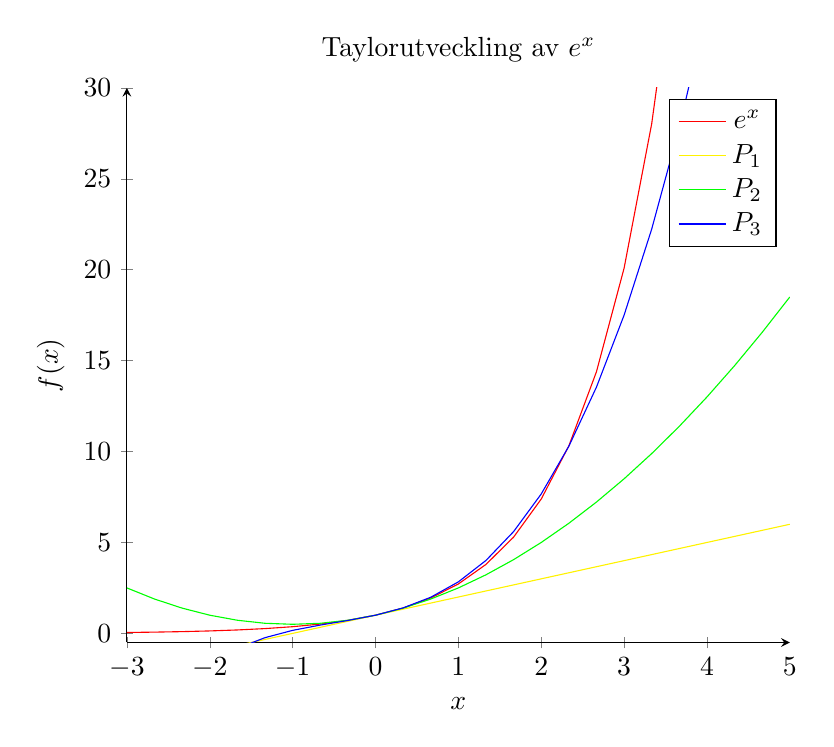
\begin{tikzpicture}
\begin{axis}[
	title=Taylorutveckling av \(e^x\),
	axis lines = left,
	xlabel=\(x\),
	ylabel={\(f(x)\)},
	xmin=-3, xmax=5,
	ymin=-0.5, ymax=30,	
]
\addplot[domain=-3:5, color=red,]{e^x};
\addlegendentry{\(e^x\)}
\addplot[domain=-3:5, color=yellow,]{1+x};
\addlegendentry{\(P_1\)}
\addplot[domain=-3:5, color=green,]{1+x+0.5*x^2};
\addlegendentry{\(P_2\)}
\addplot[domain=-3:5, color=blue,]{1+x+0.5*x^2+(1/3)*x^3};
\addlegendentry{\(P_3\)}
\end{axis}
\end{tikzpicture}
\end{center}
}

\qs{}
{
	Bestäm det 1:a Taylorpolynomet för $ f(x) = sinx $ kring $ x = \frac{\pi}{2}  $
}
\sol $ f( \frac{\pi}{2} ) = 1,\: f'(x) = cosx,\: f'( \frac{\pi}{2} ) = 0 $ 
\begin{equation*}
P_1 = \frac{ \frac{\pi}{2} }{1!} (x- \frac{\pi}{2} )
\end{equation*}

\vspace{20pt}
\qs{}
{
Bestäm Taylorpolynomen av grad $ 2,3,4, \ldots  $ osv för:
\begin{equation*}
f(x) = (x-1)^2(x-2)
\end{equation*}
}

\sol $ f(x) = (x-1)^2(x-2) = (x-1)^3-(x-1)^2,\: f(1) = 0,\: f'(1) = 0,\: f''(1) = -2 $
\begin{equation*}
P_2 = f(1) + f(1)(x-1) + \frac{f''(1)}{2!} (x-1)^2 = -(x-1)^2
\end{equation*}
$ P_3,\: P_4, \: \ldots  $ är alla $ f(x) $ då $ f $ är ett polynom av grad 3. 

\vspace{20pt}
\thm{Om $ f $ är deriverbar 2 gånger i ett intervall som innehåller $ a $ och $ x $ så gäller för något $ c $ mellan $ a $ och $ x $ att följande gäller}
{
\begin{equation*}
f(x) = f(a) + f'(a)(x-a) + \frac{f''(c)}{2!} (x-a)^2
\end{equation*}
}

\noindent
\textbf{Alltså}: Felet i den linjära approximationen, d.v.s. skillnaden mellan $ f(x) $ och $ f(a) + f'(a)(x-a) $ är precis:
\begin{equation*}
\frac{f''(c)}{2!} (x-a)^2
\end{equation*}
...för något tal $ c $ mellan $ x $ och $ a $.
Beviset baseras på medelvärdessatsen.

\vspace{20pt}
\ex{Vi approximerade tidigare $ \sqrt{2} \approx 1.5 $. Hur stort är detta fel enligt ovan? Jämför med verkliga felet. }
{
	$ \sqrt{2} \approx 1.5 $ för att tangentlinjen för $ \sqrt{x}  $ i $ x = 1 $, $ y = 1 + \frac{x-1}{2}  $ använde $ \sqrt{2} \approx P_1(2) = 1 + \frac{1}{2}  $. \textbf{Felet} måste då vara $ f(2) - P_1(2) = \frac{f''(c)}{2!} (2-1)^2 $. Utifrån det så kan vi se att felet $ \in ( - \frac{1}{8} , 0) $ 
} 

\dfn{Felet i Taylorpolynomet}
{
\textbf{Felet} i högre ordningens approximationer ges av ungefär hur nästa term i utvecklingen skulle se ut så där:
\begin{equation*}
	f(x) - P_n(x) = \frac{f^{(n+1)}(c)}{(n+1)!}(x-a)^{n+1} 
\end{equation*}
...för något punkt $ c $ mellan $ x $ och $ a $. Förutsättningen för att detta ska gälla är att $ f $ är $ n+1 $ gånger deriverbar på något intervall som innehåller både $ x $ och $ a $.\\\\

\noindent
Taylorpolynom kring origo, d.v.s. då punkten $ a = 0 $, brukar ofta kallas för \textbf{Maclaurinpolynom}.
}

\ex{Felet i approximationen $ e = e^1 \approx 1 + 1 + \frac{1}{2} = 2.5 $ ges av $ \frac{e^c}{3!}  $ för något $ c \in (0,1) $. }
{
Vi kan då i alla fall säga att:
\begin{equation*}
0 < e - 2.5 = \frac{e^c}{3!} \le \frac{3}{3!} = \frac{1}{2}  
\end{equation*}
Det \textbf{egentliga} felet är $ \approx 0.218 $ 
}

\vspace{20pt}
\qs{}
{
Bestäm Taylorpolynom av grad 2 till $ f(x) = \sqrt{x}  $ kring punkten $ x = 1 $ och använd det för att hitta ett närmevärde (som är bättre än 1.5) till $ \sqrt{2}  $. Analysera felet!
}

\sol $ f'(x) = \frac{1}{2 \sqrt{x} },\: f''(x) = - \frac{1}{4 x^{ \frac{3}{2} }}, \: f'''(x) = \frac{3}{8 x^{ \frac{5}{2} }}  $. $ a = 1 \implies f(1) = 1, \: f'(1) = \frac{1}{2}, \: f''(1) = - \frac{1}{4}, \: f'''(1) = \frac{3}{8} $.
\begin{equation*}
P_2(x) = 1 + \frac{1}{2} (x-1) - \frac{1}{8} (x-1)^2  
\end{equation*}
$ P_2(x) = 1 + \frac{1}{2}  - \frac{1}{8} = \frac{11}{8} \approx 1.375 $.\\
\textbf{Felet} kan estimieras av $ \frac{f'''(c)}{3!} (2-1)^3, \: c \in [1,2]$. $ c = 1 \implies \frac{f'''(c)}{3!} = \frac{3}{48} 1^3 = \frac{1}{16} $ som är då största approximativa felet, eftersom $ \frac{f'''(2)}{3!} (2-1)^3 < \frac{f'''(1)}{3!} (2-1)^3 $.\\
\textbf{Felet} ligger då i intervallen $ (0, \frac{1}{16} ) $     

\nt{Notera att Taylorutveckling är inte effektiv för alla funktioner. Alltså att felet \textbf{inte} minskas eller minskas segt desto flera termer vi använder}

\pagebreak

\chapter{Modul 5}
\section{Föreläsning 13 (14/02/2023)}
Integraler.\\
\noindent
I många tillämpningar uppkommer situationerna där man måste beräkna oändliga summor av längden gånger bredden. Detta kan göras med hjälp av integraler.

\dfn{Integral}
{
Så vad menar vi med?:
\begin{equation*}
\int_{a}^{b} f(x) \: dx
\end{equation*}
\textbf{Grundläggande idé}: Vi antar att $ f $ är begränsad på $ [a,b] $. Vi delar sedan in $ [a,b] $ i ett antal små delintervall och väljer en punkt i varje delintervall. På varje delintervall tar vi sedan funktionsvärdet i punkten vi har valt och multiplicerar det med delintervallens längd. Sedan summerar vi sådana areor. \textbf{Alltså, intuitivt}: Integralen ovan är arean (med tecken!) mellan grafen $ y = f(x) $, x-axeln samt vertikala linjerna $ x=a $ och $ x=b $.  

\begin{center}
	\includegraphics{integral-area}
\end{center}

Riemannsummor mot ett enda värde säger vi att $ f $ är \textbf{integrerbar} och definierar integral som detta gränsvärde:
\begin{equation*}
\int_{a}^{b} f(x) \: dx = \lim_{\Delta x_j \to 0} \sum_{j = 1}^{N} f(c_j)\:\Delta x_j 
\end{equation*}
Där vi definierar $ \Delta x_j = x_j - x_{j-1} \to 0 $
}

\pagebreak
\thm{Om $ f $ är kontinuerlig på $ [a,b] $ så är $ f $ \textbf{integrerbar} på $ [a,b] $ }
{
}

\thm{Vi kan utvidga integralbegreppet till styckvis kontinuerliga funktioner och om $ f $ är styckvis kontinuerlig på $ [a,b] $ så är $ f $ integrerbar på $ [a,b] $ }
{
}

\nt{Uppenbart från definitionen att $ f $ är kontinuerlig, att följande gäller:
\[
	(b-a) \cdot min(a,b)_f \le \int_{a}^{b} f(x) \: dx \le (b-a) \cdot  max(a,b)_f 
\]
Notera att $ min(a,b)_f $ och $ max(a,b)_f $ innebär det minsta och max värdet som funktionen $ f $ ger under intervallet $ [a,b] $  }

\ex{Skriv upp en konkret Riemannsumma till följande integral}
{
\textbf{Integralen}:
\begin{equation*}
\int_{0}^{1} x \: dx 
\end{equation*}

\textbf{Lösning}:\\
Låt $ x_i = \frac{i}{N}  $, d.v.s., $ x_0 = 0,\: x_1 = \frac{1}{N}, \: \ldots, \: x_N = \frac{N}{N} $ och $ c_i = x_i $:
\begin{equation*}
\sum_{i=1}^{N} f( \frac{i}{N} ) \frac{1}{N} = \sum_{i = 1}^{N} \frac{i}{N^2} \iff \frac{1}{N^2} \sum_{i=1}^{N} \frac{N(N+1)}{2} = \frac{1}{2} + \frac{1}{2N} \to \frac{1}{2}  
\end{equation*}
}
\nt{ \begin{equation*}
\sum_{k = 1}^{k} = \frac{k(k+1)}{2} 
\end{equation*}
}

\qs{}
{
Bestäm valfri Riemannsumma till integralen:
\begin{equation*}
\int_{0}^{1} x^2 \: dx 
\end{equation*}
och förklara ditt val av intervall och punkter.
}

\sol 
\begin{equation*}
c_i = x_i = \frac{1}{N},\: N \to \infty \implies \int_{0}^{1} x^2 \: dx \approx \sum_{i=1}^{N} ( \frac{i}{N} )^2  \frac{1}{N}  
\end{equation*}
T.ex med $ N=3,\: x_0 = 0,\:x_1 = \frac{1}{2},\: x_2 = 1,\: c_1 = \frac{1}{2},\:c_2 = 1 $. Då får vi:
\begin{equation*}
	( \frac{1}{2} )^2 \cdot \frac{1}{2} + 1^2 \cdot \frac{1}{2}  = \frac{1}{8} + \frac{1}{2} 
\end{equation*} 

\noindent
Intervaller har följande egenskaper:
\begin{align*}
	&\int_{a}^{b} f(x)+g(x) \: dx = \int_{a}^{b} f(x) \: dx + \int_{a}^{b} g(x) \: dx\\
	&\int_{a}^{b} kf(x) \: dx = k \int_{a}^{b} f(x) \: dx\\
	&\int_{a}^{b} f(x) \: dx + \int_{b}^{c} f(x) \: dx = \int_{a}^{c} f(x) \: dx\\
	&\int_{a}^{b} f(x) \: dx \le \int_{a}^{b} g(x) \: dx,\: \text{om } f \le g \in [a,b]\\
	&|\int_{a}^{b} f(x) \: dx| \le \int_{a}^{b} f(x) \: dx\: \text{ (triangelolikheten)}   
\end{align*}

\thm{Medelvärdesatsen för integraler}
{
	Om $ f $ är kontinuerlig på $ [a,b] $ så finns ett tal $ c $ mellan $ a $ och $ b $ sådant att:
	\begin{equation*}
	\int_{a}^{b} f(x) \: dx = f(c)(b-a) 
	\end{equation*}
	Talet $ c $ kallas för \textbf{medelvärdet} av $ f $ på $ [a,b] $. Beviset bygger på den "vanliga medelvärdesatsen" för kontinuerliga funktioner.\\\\


\textbf{Bevis}:
Medelvärdet är:
\begin{equation*}
\frac{1}{b-a} \int_{a}^{b} f(x) \: dx 
\end{equation*}
Medelvärdesatsen för integraler säger att $ f $ antar medelvärdet. Vi vet att:
\begin{equation*}
min(b,a)_f \cdot (b-a) \le \int_{a}^{b} f(x) \: dx \le max \cdot max(b,a)_f \cdot (b-a)
\end{equation*}
Alltså medelvärdet måste vara mellan $ min(b,a)_f $ och $ max(b,a)_f $. Satsen om mellanliggandevärde implicerar att $ f $ antar alla värden i intervallen $ [min(b,a)_f, max(b,a)_f] $ eftersom $ f $ är kontinuerlig. 
}

\ex{}
{
Låt:
\begin{align*}
	f(x) &= -1,\:\: x \in [-1,0)\\
	f(x) &= 0, \:\: x \in [0,1]\\
	f(x) &= 1, \:\: x \in (1,2]
\end{align*}
1) Vad är $ f $:s medelvärde på $ [0,2] $? Gäller medelvärdesatsen för $ f $ på $ [0,2] $?\\
Enligt 5.1.3 och om medelvärdesatsen gäller så existerar $ c \in [0,2]	 $ så att $ 1 = f(c) \cdot (2-0) $, alltså medelvärdet $ f(c) $ borde vara $ f(c) = \frac{1}{2}  $. Detta går ej! Alltså medelvärdessatsen kräver kontinuitet!\\\\
}

\dfn{Huvudsatsen}
{
Huvudsatsen säger att derivatan och integraler är motsatta operationer och att man kan räkna ut integraler genom att anti-deriviera eller hitta primitiv funktion.
\begin{equation*}
\int_{a}^{b} f(x) \: dx = F(b) - F(a),\:\: F'(x) = f(x) 
\end{equation*}
}

\dfn{Primitiva funktioner}
{
Vi säger att $ F $ är en \textbf{primitiv funktion} till $ f $ på ett intervall $ I $ om $ F'(x) = f(x) $ på intervallen $ I $.
}

\nt{En primitiv funktion $ F $ är \textbf{aldrig} unik. $ F(x) + C, C \in \mathbb{C} $ är också en primitiv funktion.}
\noindent
Om $ F $ och $ G $ är primitiva funktioner så säger vi:
\begin{equation*}
\frac{d}{dx} F-G = 0,\: \in I
\end{equation*}
...och detta betyder att $ F(x) = G(x) + C $ och vi kommer använda notationen:
\begin{equation*}
\int_{}^{} f(x) \: dx = F(x) + C, \: ( x \in I)
\end{equation*}
Integralen utan värden brukar kallas för \textbf{indefinita} eller \textbf{obestämda} integralen av $ f $.

\dfn{Analysens huvudsats}
{
	EN: \textit{The Fundamental Theorem of Calculus}\\
	Antag att $ f $ är kontinuerlig på $ [a,b] $. Då gäller:
	\textbf{1)}: Funktionen $ F(x) = \int_{a}^{x} f(t) \: dt $ är en primitiv funktion till $ f $, d.v.s. $ \frac{d}{dx} F(x) = f(x) $\\
	\textbf{2)}: Om $ G $ är någon primitiv funktion till $ f $, så är:
\begin{equation*}
\int_{a}^{b} f(t) \: dt = G(b) - G(a)
\end{equation*}

Det första delen kan bevisas genom:
\begin{equation*}
\lim_{h \to 0} \frac{F(x+h)-F(x)}{h}  = \frac{ \int_{a}^{x+h} f(x) \: dx - \int_{a}^{x} f(x) \: dx }{h} = \frac{ \int_{x}^{x+h} f(x) \: dx }{h} 
\end{equation*}
Enligt medelvärdesatsen för integraller så medförs följande:
\begin{equation*}
\frac{hf(c_h)}{h} = f(c_h) \to f(x)
\end{equation*}
...då $ h \to 0 $ och $ c_h \in [x, x+h]$ 
}

\ex{}
{
Bestäm:
\begin{equation*}
\frac{d}{dx} \int_{-5}^{x} f(t) \: dt 
\end{equation*}
Vi vet från analysens fundamentalsats att $ F(x) = \int_{-5}^{x} t \: dt  $ som är primitiva funktionen till $ f(x) = x $. Alltså:
\begin{equation*}
\frac{d}{dx} F(x) = \frac{d}{dx} \int_{-5}^{x} t \: dt = x 
\end{equation*}
}

\ex{}
{
Bestäm:
\begin{equation*}
	\frac{d}{dt} \int_{-t^2}^{-t^3} e^{x^2} \: dx 
\end{equation*}
Vi vet att att om $ F $ är en primitiv funktion till $ e^{x^2} $ så betyder det att:
\begin{equation*}
	\int_{-t^2}^{t^3} e^{x^2} \: dx = F(t^3) - F(-t^2) 
\end{equation*}
Genom att deriviera utrycket med hänsyn till $ t $, så får vi följande:
\begin{equation*}
	\frac{d}{dt} \int_{-t^2}^{t^3} e^{x^2} \: dx = \frac{d}{dt} F(t^3) - \frac{d}{dt} F(-t^2) \iff f(t^3) 3t^2 - f(-t^2) (-2t) 
\end{equation*}
$ f(t) = e^{x^2} $, alltså slutliga utrycket har formen:
\begin{equation*}
	e^{(t^3)^2}3t^2 - e^{(-t^2)^2}(-2t) = e^{t^6} 3t^2 + e^{t^4} 2t
\end{equation*}
}
\ex{}
{
Varför är följande summa en bra approximation på $ ln2 $ när $ N $ är stort?
\begin{equation*}
\sum_{j = 1}^{N} \frac{1}{1 + \frac{i}{N} } \cdot \frac{1}{N} 
\end{equation*}
Med $ c_i = x_i = \frac{i}{N},\: i = 1, \ldots , N $ fick vi att Riemannsumman är:
\begin{equation*}
\sum_{i = 1}^{N} f( \frac{i}{N} ) \frac{1}{N} 
\end{equation*}
Dock i vårt fall när $ f(x) = \frac{1}{1+x}  $ blir detta:
\begin{equation*}
\sum_{i = 1}^{N} \frac{1}{1 + \frac{i}{N} } \cdot \frac{1}{N} 
\end{equation*}
Vi vet då att $ \int_{0}^{1} \frac{1}{1+x}  \: dx = \lim_{N \to \infty} \sum_{i = 1}^{N} \frac{1}{1 + \frac{i}{N} } \frac{1}{N}  $. Eftersom $ f $ är kontinuerlig på intervallen $ [0,1] $ och därmed integrerbar. Eftersom $ \frac{d}{dx}ln(1+x) = \frac{1}{1+x}  $ så har vi att:
\begin{equation*}
	\int_{0}^{1} \frac{1}{1+x}  \: dx = [ln(1+x)]_{0}^{1} = ln(2) - ln(1) = ln(2) 
\end{equation*}
Alltså gränsvärdet av Riemannsumman är ln2, då $ N \to \infty $ 
}

\qs{}
{
Bestäm:
\begin{equation*}
\frac{d}{ds} \int_{s}^{e^s} sin(x^2) \: dx 
\end{equation*}
}

\sol Om $ F(x) = \int_{}^{} sin(x^2) \: dx  $, så är $ \int_{s}^{e^s} sin(x^2) \: dx = F(e^s) - F(s)  $. Då får vi följande:
\begin{equation*}
\frac{d}{ds} \int_{e^s}^{s} sin(x^2) \: dx = \frac{d}{ds} F(e^s) - \frac{d}{ds} F(s) \implies  e^s f(e^s) - f(s)
\end{equation*}
Där $ f(x) = sin(x^2) $. Alltså utrycket omvandlas till:
\begin{equation*}
	e^s sin((e^s)^2) - sin(e^s)
\end{equation*}

\vspace{20pt}
\qs{}
{
Bestäm:
\begin{equation*}
	\int_{0}^{1} \frac{1}{1+x^2}  \: dx
\end{equation*}
(Tips: Kom ihåg era trigonometriska funktioner!)
}

\sol Vi vet att $ \frac{d}{dx} arctan(x) = \frac{1}{1+x^2}  $, alltså enligt huvudsatsen så får vi följande:
\begin{equation*}
\int_{0}^{1} \frac{1}{x^2+1}  \: dx = arctan(1) - arctan(0) 
\end{equation*}
Vi vet att $ arctan(1) = \frac{\pi}{4}   $ och $ arctan(0) = 0 $. Alltså \textbf{svaren} är $ \frac{\pi}{4}  $

\vspace{20pt}
\qs{}
{
Bestäm:
\begin{equation*}
\lim_{N \to \infty} \sum_{j = 1}^{N} \frac{ \frac{1}{N} }{1 + ( \frac{j}{N} )^2} 
\end{equation*}
}

\sol Med $ f(x) = \frac{1}{1+x^2}  $ fås Riemannsumman för $ \int_{0}^{1} f(x) \: dx  $ till $ \sum_{j = 1}^{N} \frac{1}{1 + ( \frac{j}{N} )^2} \cdot \frac{1}{N}  $. Alltså gränsvärdet kan tas från förra frågan, som då är $ \frac{\pi}{4}  $.

\pagebreak
\section{Föreläsning 14 (15/02/2022)}
Variabelsubstitution, partiellintegrering.\\\\

\noindent
Arean av området $ g \le y \le f $, $ a \le x \le b $ kan beräknas genom skillnaden mellan areorna som ligger under $ f $ och $ g $:
\begin{equation*}
A = \int_{a}^{b} (f-g) \: dx 
\end{equation*}

\ex{Bestäm arean för området som begränsas av kurvorna $ y = x^3 $ och $ y = x^2 $  }
{
\begin{equation*}
	A = \int_{0}^{1} (x^2-x^3) \: dx = [ \frac{x^3}{3} - \frac{x^4}{4}  ]_{0}^{1} = \frac{1}{3} - \frac{1}{4} 
\end{equation*}
Funktionerna $ x^3 $ och $ x^2 $ skär varann i $ x= 0 $ och $ x= 1 $ . På intervallet $ [0,1] $ gäller att $ x^2 \ge x^3 $. Arean av området mellan motsvarande funktionsgraferr ges av integralen ovan. 

\begin{tikzpicture}
\begin{axis}[
	title=\(f(x)\) och \(g(x)\),
	axis lines = left,
	xlabel=\(x\),
	ylabel={\(y\)},
	xmin=-1, xmax=2,
	ymin=-0.5, ymax=5,	
]
\addplot[domain=-1:2, name path=f, color=red,]{x^3};
\addlegendentry{\(x^3\)}

\addplot[domain=-1:2, name path=g, color=blue,]{x^2};
\addlegendentry{\(x^2\)}

\addplot[purple, opacity=0.4,] fill between[of=f and g, soft clip={domain=0:1}];

\end{axis}
\end{tikzpicture}
}

\subsection{Variabelsubstitution}
\dfn{Variabelsubstitution}
{
\begin{equation*}
\int_{a}^{b} f(g(x))g'(x) \: dx = \int_{g(a)}^{g(b)} f(u) \: du  
\end{equation*}
\textbf{Anledning}: $ F(g(x)) $ är primitiv till $ f(g(x))g'(x) $. Detta pga:
\begin{equation*}
\frac{d}{dx}F(g(x)) = F'(g(x)) g'(x) = f(g(x))g'(x)
\end{equation*}
Det betyder att:
\begin{equation*}
\int_{a}^{b} f(g(x))g'(x) \: dx = F(g(b)) - F(g(a))
\end{equation*}
\textbf{I praktiken}:\\
Vi antar att en funktion i integralen är $ u $, d.v.s. $ u = g(x) \implies du = g'(x) dx \iff dx = \frac{du}{g'(x)} $. Vi ersätter termerna i integralen och sätter gränserna av integralen från $ a $ och $ b $ till $ g(a) $ och $ g(b) $. Alltså:
\begin{equation*}
\int_{a}^{b} f(g(x))g'(x) \: dx = \int_{g(a)}^{g(b)} f(u) g'(x) \frac{1}{g'(x)} \: du = \int_{g(a)}^{g(b)} f(u) \: du    
\end{equation*}
}

\ex{}
{
Bestäm:
\begin{equation*}
\int_{0}^{ \frac{\pi}{2} } \frac{cosx}{1 + sinx}  \: dx 
\end{equation*}
\textbf{Lösning}:
\begin{equation*}
u = sinx,\:\: du = cosx\:dx \iff \frac{du}{cosx} = dx
\end{equation*}
Detta medför:
\begin{equation*}
	\int_{u(0)}^{u(1)} \frac{1}{1+u}  \: du = [ ln(1+u) ]_{0}^{1} = ln2-ln1 = ln2
\end{equation*}
\textbf{OBS}: $ ln(1+sinx) $ är primitiva funktion till $ \frac{cosx}{1+sinx}  $
}

\vspace{20pt}
\qs{}
{
Bestäm:
\begin{equation*}
	\int_{0}^{1} x^2e^{x^3} \: dx 
\end{equation*}
}
\sol Vi låter $ u = x^3 \implies \frac{du}{dx} 3x^2 \iff \frac{du}{3x^2} = dx $. Vi sätter in integralens gränsvärde i $ u $: $ u(0) = 0 $ och $ u(1) = 1 $. Vi substiterar allt:
\begin{equation*}
	\int_{u(0)}^{u(1)} x^2 e^u \frac{1}{3x^2}  \: du = \frac{1}{3} \int_{0}^{1} e^u \: du = [e^u]_{0}^{1} = e-1  
\end{equation*}

\pagebreak
\qs{}
{
Bestäm:
\begin{equation*}
\int_{}^{} tanx \: dx 
\end{equation*}
Tips: Skriv ut $ tanx = \frac{sinx}{cosx}  $
}

\sol Vi sätter in $ u = cosx \implies \frac{du}{dx} = -sinx \iff -\frac{du}{sinx} = dx  $:
\begin{equation*}
	\int_{}^{} tanx \: dx = \int_{}^{} \frac{sinx}{cosx}  \: dx = \int_{}^{} \frac{sinx}{u} \frac{1}{-sinx}  \: du = -\int_{}^{}  \: du = -ln|u| +C   
\end{equation*}
Alltså primitiva funktionen till $ tanx $ är $ -ln|cosx|+C $ 

\vspace{20pt}
\subsection{Partiell integration}
\dfn{Partiell integration}
{
\begin{equation*}
	\int_{a}^{b} f(x)g(x) \: dx = [F(x)g(x)]_{a}^{b} - \int_{a}^{b} F(x)g'(x) \: dx
\end{equation*}
\textbf{Villkor}: $ F $ och $ g $ har kontinuerliga derivator på $ [a,b] $ och $ F' = f $.

\textbf{Bevis}:\\
Produktregeln för derivator ger att:
\begin{equation*}
\frac{d}{dx} F(x)g(x) = F'(x)g(x) + F(x)g'(x)
\end{equation*}
\textbf{Partiell integration} utan gränser:
\begin{equation*}
\int_{}^{} f(x)g(x) \: dx = F(x)g(x) - \int_{}^{} F(x)g'(x) \: dx  
\end{equation*}

}

\ex{}
{
Beräkna med hjälp av partiell integration:
\begin{equation*}
\int_{0}^{ \frac{\pi}{2} } x \cdot sinx \: dx 
\end{equation*}
\textbf{Lösning}:
Vi sätter $ g(x) = x $ och $ f(x) = sinx $:
\begin{equation*}
	\int_{0}^{ \frac{\pi}{2} } f(x)g(x) \: dx = \int_{0}^{ \frac{\pi}{2} } F(x)g(x) \: dx - \int_{0}^{ \frac{\pi}{2} } F(x)g'(x) \: dx = [ -cosx \cdot x]_{0}^{ \frac{\pi}{2} } - \int_{0}^{ \frac{\pi}{2} } -cosx \cdot 1 \: dx = [ -cosx \cdot x]_{0}^{ \frac{\pi}{2} } - [-sinx ]_{0}^{ \frac{\pi}{2} }    
\end{equation*}
Utrycket ovan evalueras till $ sin( \frac{\pi}{2} ) - sin(0) = 1 $ 
}

\pagebreak
\ex{}
{
Bestäm med hjälp av partiell integration:
\begin{equation*}
\int_{}^{} lnx \: dx 
\end{equation*}
\textbf{Lösning}: Vi antar $ f(x) = 1 $ och $ g(x) = lnx $:
\begin{equation*}
\int_{}^{} f(x)g(x) \: dx = x \cdot lnx - \int_{}^{} x \cdot \frac{1}{x}  \: dx = xlnx-x + C    
\end{equation*}
}

\vspace{20pt}
\qs{}
{
Bestäm:
\begin{equation*}
\int_{1}^{4} \sqrt{x} lnx \: dx 
\end{equation*}
}
\sol Vi sätter $ f(x) = \sqrt{x}  $ och $ g(x) = lnx $:
\begin{equation*}
	\int_{1}^{4} f(x)g(x) \: dx = [2 \frac{x^{ \frac{3}{2} }}{3} lnx  ]_{1}^{4} - \int_{1}^{4} \frac{2x^{ \frac{3}{2} }}{3} \cdot \frac{1}{x}   \: dx \implies [2 \frac{x^{ \frac{3}{2} }}{3} lnx ]_{1}^{4}- \frac{2}{3} [2 \frac{x^{ \frac{3}{2} }}{3}]_{1}^{4}   
\end{equation*}

\vspace{20pt}
\qs{}
{
Bestäm:
\begin{equation*}
\int_{}^{} arcsinx \: dx 
\end{equation*}
}

\sol Vi sätter $ f(x) = 1 $ och $ g(x) = arcsinx $:
\begin{equation*}
\int_{}^{} arcsinx \: dx = x \cdot arcsinx - \int_{}^{} \frac{x}{ \sqrt{1 - x^2}  }  \: dx  
\end{equation*}
$ \int_{}^{} \frac{x}{ \sqrt{1 - x^2} }  \: dx $ kan lösas genom att sätta $ u = \sqrt{1 - x^2}  \implies \frac{du}{dx} = -\frac{x}{ \sqrt{1 - x^2}  } \iff - \frac{ \sqrt{1-x^2} }{x}\:du =dx   $:
\begin{equation*}
\int_{}^{} \frac{x}{ \sqrt{1-x^2} }  \: dx = \int_{}^{} -1 \: du = -u + C = - \sqrt{1-x^2} + C  
\end{equation*}
\textbf{Alltså}:
\begin{equation*}
\int_{}^{} arcsinx \: dx = x \cdot arcsinx + \sqrt{1 - x^2} + C 
\end{equation*}

\pagebreak
\section{Föreläsning 15  (16/02/2022)}
Partiellbråksuppdelning och integrationstekniker.\\\\

\noindent
Ibland kan det hända att vi får tillbaka något som påminner om den ursprungliga integralen när vi partiellintegrerar upprepade gånger. Då ska man inte misströsta! Då kan vi lösa ut den sökta integralen ur ekvationen.

\ex{}
{
Bestäm integralen:
\begin{equation*}
	\int_{}^{} e^x sinx\: dx 
\end{equation*}
\textbf{Lösning}:
\begin{equation*}
	\int_{}^{} e^x sinx \: dx = e^xsinx - \int_{}^{} e^x cosx \: dx = e^xsinx -( e^xcosx + \int_{}^{} e^x sinx \: dx ) = -\int_{}^{} e^x sinx \: dx - e^x cosx + e^x sinx  
\end{equation*}
Vi kan tro att vi har inte kommit någonstans, men låt oss sätta $ I = \int_{}^{} e^x sinx \: dx  $:
\begin{align*}
	I &= -I + e^x(sinx-cosx) \\
	I &= \frac{e^x(sinx-cosx)}{2} 
\end{align*}
}

\vspace{20pt}
\noindent
\textbf{Trigonometriska integraler} av typen $ \int_{}^{} sin^nx cos^nx \: dx $:
\begin{itemize}
	\item Om $ m $ eller $ n $ är udda kan vi hantera dessa med hjälp av trigonometriska ettan, t.ex:
	\begin{equation*}
	\int_{}^{} sin^3xcos^4x \: dx = \int_{}^{} (1-cos^2x)cos^4xsinx \: dx
	\end{equation*}
	Som kan hanteras med substitutionen $ u = cosx $
	\item Om både $ m $ eller $ n $ är jämna så kan integralen reduceras till polynom i $ cos2x $ genom formlerna:
	\begin{equation*}
	cos^2x = \frac{1}{2} (1 + cos2x),\:\: sin^2x = \frac{1}{2} (1-cos2x)
	\end{equation*}
	Se kapitel 5.6 i boken för trigonometriska integraler.
\end{itemize}

\ex{När $ m $ eller $ n $ är udda}
{
\textbf{Bestäm}:
\begin{equation*}
\int_{}^{} sin^3xcos^4x \: dx = \int_{}^{} (1-cos^2x)cos^4x sinx \: d 
\end{equation*}
Vi gör substitutionen $ u = cosx,\:\: du = -sinx\:dx $:
\begin{equation*}
- \int_{}^{} (1-u^2)u^4 \: du = \int_{}^{} u^6-u^4 \: du = \frac{u^7}{7} - \frac{u^5}{5} + C \implies  \frac{cos^7x}{7} - \frac{cos^5x}{5} + C   
\end{equation*}
}

\pagebreak
\ex{Om $ m $ och $ n $ är jämna}
{
\textbf{Bestäm}:
\begin{equation*}
\int_{}^{} sin^2x+cos^2x \: dx = \int_{}^{} \frac{1}{4} (1+cos2x)(1-cos2x) \: dx = \frac{1}{4} \int_{}^{} 1-cos^2x \: dx   
\end{equation*}
Vi vet att $ cos^22x = \frac{1}{2} (1+cos4x) $:
\begin{equation*}
\implies \frac{1}{4} \int_{}^{} 1- \frac{1}{2} (1+ cos4x) \: dx = \frac{1}{8} \int_{}^{} 1 - cos4x \: dx = \frac{1}{8} (x - \frac{sin4x}{4} ) + C  
\end{equation*}
}

\qs{}
{
\textbf{Bestäm}:
\begin{equation*}
\int_{0}^{ \frac{\pi}{2} } sin^4xcos^3x \: dx
\end{equation*}
}

\sol
\begin{equation*}
\int_{0}^{ \frac{\pi}{2} } sin^4xcos^3x \: dx = \int_{0}^{ \frac{\pi}{2} } (1-sin^2x)cosx sin^4x \: dx  
\end{equation*}
Vi gör substitutionen $ u = sinx,\:\: du = cosx\:dx $:
\begin{equation*}
	\int_{0}^{ \frac{\pi}{2} } (1-sin^2x)cosxsin^4x \: dx = \int_{sin(0)}^{sin( \frac{\pi}{2} )} (1-u^2)u^4 \: du = \int_{0}^{1} u^4 - u^6 \: du = [\frac{u^5}{5} - \frac{u^7}{7}]_{0}^{1} = \frac{1}{5} - \frac{1}{7} - [0 - 0] \implies \frac{2}{35}     
\end{equation*}

\vspace{20pt}
\qs{}
{
\textbf{Bestäm}:
\begin{equation*}
\int_{}^{} \frac{1}{x^2+2x+2}  \: dx 
\end{equation*}
}
\sol Vi sätter $ x^2+2x+2 = (x+1)^2+1 $:
\begin{equation*}
\int_{}^{} \frac{1}{(x+1)^2+1}  \: dx 
\end{equation*}
Vi göt substitutionen $ u = x+1,\:\: du = dx $:
\begin{equation*}
\int_{}^{} \frac{1}{u^2+1}  \: du = arctan(u) \implies arctan(x+1) +C 
\end{equation*}

\subsection{Partiellbråksuppdelning}
\dfn{Partiellbråksuppdelning}
{
Görs vid rationella integrander, d.v.s. integrander på formen:
\begin{equation*}
\frac{P(x)}{Q(x)} 
\end{equation*}
Detta görs \textbf{endast} om $ P(x) $ har lägre grad än $ Q(x) $. Det existerar olika fall för att bestämma partiellbråksuppdelningen:
\begin{itemize}
	\item \textbf{Situation 1}: Enkla \textbf{olika} faktorer:
	\begin{equation*}
		\frac{P(x)}{(x-a_1) \ldots (x-a_n)}  = \frac{A_1}{x-a_1} + \ldots + \frac{A_n}{x-a_n} 
	\end{equation*}
	\item \textbf{Situation 2}: Upprepade enkla (linjära) rötter. Om $ \frac{1}{x-a} $ är uppdelad $ k $ gånger får vi för denna faktor ansätta:
	\begin{equation*}
		\frac{A_1}{x-a} + \frac{A_2}{(x-a)^2} + \ldots + \frac{A_k}{(x-a)^k} 
	\end{equation*}
	\item \textbf{Situation 3}: Irreducibla (komplexa rötter). För en faktor som $ \frac{1}{x^2+a^2}  $ ansätter vi termen:
	\begin{equation*}
		\frac{Ax+B}{x^2+a^2}
	\end{equation*}
	Om det står $ x^2+bx+c $ istället i nämnaren kan vi kvadratkomplettera och byta variabler.
	\item \textbf{Situation 4}: Upprepade irreducibla faktorer. För $ \frac{1}{(x^2+a^2)^k}  $ ansätter vi termerna:
	\begin{equation*}
		\frac{A_1x+B_1}{x^2+a^2} + \frac{A_2x+B_2}{(x^2+a^2)^2} + \ldots + \frac{A_kx+B_k}{(x^2+a^2)^k}  
	\end{equation*}
	
\end{itemize}
\textbf{Poängen} med allt det där är att vi kan lätt integrera funktioner på formen:
\begin{equation*}
\frac{1}{x+C},\: C \in \mathbb{R}
\end{equation*}

}

\ex{}
{
\begin{equation}
\frac{3x}{(x-1)(x-2)} = \frac{A}{x-1} + \frac{B}{x-2} = \frac{A(x-2)+B(x-1)}{(x-1)(x-2)}  
\end{equation}
Alltså, $ 3x = A(x-2)+B(x-1) $   som kan skrivas om till en ekvationssystem:
\begin{align*}
	A+B &= 3\\
	-2A+-B &= 0
\end{align*}
Genom att lösa ut ekvationssystemen så får vi $ A = -3 $ och $ B = 6 $ som vi kan sätta tillbaka i ekvation 5.1:
\begin{equation*}
\frac{3x}{(x-1)(x-2)} = - \frac{3}{x-1} + \frac{6}{x-2}  
\end{equation*}
}

\pagebreak

\ex{}
{
\begin{equation*}
\frac{3x+1}{(x-1)^2(x-2)} = \frac{A}{x-1} + \frac{B}{(x-1)^2} + \frac{C}{x-2} 
\end{equation*}
Alltså:
\begin{equation*}
3x+1 = A(x-1)^2+B(x-1)(x-1)+C(x-2)
\end{equation*}
\begin{itemize}
	\item $ x = 1 \implies 4 = 0 + 0 - C, \:\: C = -4$\\
	\item $ x = 2 \implies 7 = A $
	\item $ x^2 $ termerna ska vara 0 $ \implies 0 = A+B \iff B=-A = -7 $
\end{itemize}
\textbf{Slutsatsen}: Om man vill integrera:
\begin{equation*}
\int_{}^{} \frac{3x+1}{(x-1)^2(x-2)}  \: dx 
\end{equation*}
...så måste man integrera:
\begin{equation*}
-7 \int_{}^{} \frac{1}{x-1}  \: dx - 4 \int_{}^{} \frac{1}{(x-1)^2}  \: dx + 7 \int_{}^{} \frac{1}{x-2}  \: dx   
\end{equation*}
...som i sin tur blir:
\begin{equation*}
7ln|x-1|+7ln|x-2| + 4(x-1)^{-1} + C
\end{equation*}

}

\ex{}
{
\begin{equation*}
\frac{2x}{(x-1)(x^2+1)} = \frac{A}{x-1} + \frac{Bx+C}{x^2+1}  
\end{equation*}
Alltså $ 2x = A(x^2+1) + (Bx+C)(x-1)$
\begin{itemize}
	\item $ x = 1 \implies 2 = 2A + 0,\:\: A = 1 $
	\item $ x^2 $ termerna $ \implies 0 = A + B,\:\: B = -A = -1 $
	\item konstanta termerna $ \implies 0 = A - C \implies C = A = 1 $  
\end{itemize}
Så integralen av:
\begin{equation*}
\frac{2x}{(x-1)(x^2+1)} 
\end{equation*}
...blir:
\begin{equation*}
\int_{}^{} \frac{1}{x-1}  \: dx - \int_{}^{} \frac{x+1}{x^2+1}  \: dx = ln|x-1| +arctan(x) = - \frac{1}{2} ln|x^2+1| + C 
\end{equation*}
}

\ex{}
{
\begin{equation*}
\frac{x^3+4x^2+x+1}{(x-1)(x-2)^2(x^2+1)^2} = \frac{A}{x-1} + \frac{B}{x-2} + \frac{C}{(x-2)^2} + \frac{Dx+E}{x^2+1} + \frac{Fx+G}{(x^2+1)^2} 
\end{equation*}

}

Basfallen för partiellbråkuppdelning:
\begin{align*}
	&\int_{}^{} \frac{1}{ax+b}  \: dx = \frac{1}{a} ln|ax+b|+C\\
	& \int_{}^{} \frac{x}{x^2+a^2}  \: dx = \frac{1}{2} ln(x^2+a^2)+C\\
	& \int_{}^{} \frac{x}{x^2-a^2}  \: dx = \frac{1}{2} ln|x^2-a^2|+C\\
	& \int_{}^{} \frac{1}{x^2+a^2}  \: dx = \frac{1}{a} arctan( \frac{x}{a} ) + C\\
	& \int_{}^{} \frac{1}{x^2-a^2}  \: dx = \frac{1}{2a} ln| \frac{x-a}{x+a} | + C   
\end{align*}

\vspace{20pt}
\qs{}
{
\textbf{Bestäm}:
\begin{equation*}
\int_{}^{} \frac{1}{x^2+x}  \: dx 
\end{equation*}
}

\sol Integralen är ekvivalent med:
\begin{equation*}
\int_{}^{} \frac{1}{x(x+1)}  \: dx \implies \int_{}^{} \frac{A}{x} + \frac{B}{x+1}  \: dx  
\end{equation*}
Vi får att $ A(x+1) + Bx = 1 $:
\begin{align*}
	A + B &= 0 \\
	A = 1
\end{align*}
...alltså $ B = -A = -1 $. Integralen blir då:
\begin{equation*}
\int_{}^{} \frac{1}{x} - \frac{1}{x+1}  \: dx = ln|x| - ln|x+1| + C 
\end{equation*}

\vspace{20pt}
\qs{}
{
\textbf{Bestäm}:
\begin{equation*}
\int_{1}^{2} \frac{1}{(x-1)(x^2-2x+5)}  \: dx 
\end{equation*}
}
\sol Vi tillämpar kvadratkomplettering $ x^2-2x+5 = (x-1)^2 + 4 $:
\begin{equation*}
\frac{1}{(x-1)(x^2-2x+5)} = \frac{1}{(x-1)((x-1)^2+4)} 
\end{equation*}
Därefter vi gör en u-substitution och sätter $ u = x-1,\:du = dx,\: x = 1 \implies u = 0,\: x = 2 \implies u = 1 $:
\begin{equation*}
\int_{0}^{1} \frac{1}{u} \cdot \frac{1}{u^2+4}  \: du = \int_{0}^{1} \frac{A}{u} + \frac{Bu+C}{u^2+4}  \: du  
\end{equation*}
Från högra sidan så får vi att $ 1 = A(u^2+4) + u(Bu+C)$:
\begin{itemize}
	\item $ u =0 \implies 1 = Au,\: A = \frac{1}{4}  $
	\item $ u $  termer $ \implies 0 = C $
	\item $ u^2 $ termer $ \implies 0 = A + B,\:B = -\frac{1}{4}  $  
\end{itemize}
Då kan vi skriva om integralen till den nedan:
\begin{equation*}
	\frac{1}{4}  \int_{0}^{1} \frac{1}{u}  \: du - \frac{1}{4} \int_{0}^{1} \frac{u}{u^2+u}  \: du = \frac{1}{4} [lnu]_{0}^{1} - \frac{1}{8} [ln(u^2+u)]_{0}^{1}   
\end{equation*}

\subsection{Inversa substitutioner}
Om en integral innehåller $ \sqrt{a^2-x^2}  $ och där $ a > 0 $, så \textbf{använd} $ u = arcsin( \frac{x}{a}  ) $

\ex{}
{
\textbf{Bestäm}:
\begin{equation*}
	\int_{}^{} \frac{1}{(1-x^2)^{ \frac{3}{2}  }}  \: dx 
\end{equation*}
...vi sätter $ u = arcsin(x)$:
\begin{equation*}
	\int_{}^{} \frac{1}{(1-x^2)^{ \frac{3}{2}  }}  \: dx = tan(u) + C 
\end{equation*}


}

\vspace{20pt}
\noindent
Integraler som innehåller $ \sqrt{a^2+x^2}  $ där $ a > 0 $, \textbf{använd} $ u = arctan( \frac{x}{a} ) $.

\ex{}
{
\textbf{Bestäm}:
\begin{equation*}
\int_{}^{} \frac{1}{(4+x^2)^2}  \: dx  
\end{equation*}
...vi sätter $ u = arctan( \frac{x}{2} ) $:
\begin{equation*}
\int_{}^{} \frac{1}{(4+x^2)^2}  \: dx = \frac{1}{8} \int_{}^{} cos^2u \: du  
\end{equation*}

}

\pagebreak
\chapter{Modul 6}
\section{Föreläsning 16 (20/02/2023)}
Generaliserade integraler.\\

\ex{Beräkna arean av det område som ligger mellan kurvorna $ y = 1 $ och $ y = \frac{x^2}{x^2-1}  $, för $ x $ i intervallet $ 2 \le x \le R $, för $ R \ge 2 $   }
{
Vad händer med arean om vi låter $ R \to \infty $? Vi använder att:
\begin{equation*}
	\frac{1}{x^2-1} = \frac{1}{2} \frac{1}{x-1} - \frac{1}{2} \frac{1}{x+1} 
\end{equation*}
\begin{tikzpicture}
\begin{axis}[
	title=,
	axis lines = left,
	xlabel=\(x\),
	ylabel={\(y\)},
	xmin=0, xmax=100,
	ymin=0, ymax=1.5,	
]
	\addplot[domain=0:1000, color=red,]{1+1/(x^2-1)};
\addlegendentry{\(x^2/(x^2-1)\)}
\addplot[domain=0:1000, color=blue,]{1};
\addlegendentry{\(1\)}

\end{axis}
\end{tikzpicture}
\\
Arean mellan kurvorna ges av:
\begin{equation*}
\int_{2}^{R} \frac{x^2}{x^2-1} -1 \: dx = \int_{2}^{R} \frac{1}{x^2-1}  \: dx = \frac{1}{2} \int_{2}^{R} \frac{1}{x-1} - \frac{1}{x+1}  \: dx   
\end{equation*}
\begin{equation*}
	\frac{x^2}{x^2-1}  - \frac{x^2-1}{x^2-1} = \frac{1}{x^2-1} \implies \frac{1}{2} [ ln(x-1) - ln(x+1) ]_{2}^{R}  = \frac{1}{2} [ln( \frac{x-1}{x+1} ]_{2}^{R} = - \frac{1}{2} ln( \frac{1}{3} ) = \frac{1}{2} ln(3) 
\end{equation*}
}

\pagebreak
\ex{}
{
\begin{equation*}
	\int_{1}^{ \infty} \frac{1}{x}  \: dx = \lim_{R \to \infty} \int_{1}^{R} \frac{1}{x}  \: dx = \lim_{R \to \infty} [lnx]_{1}^{R} = \lim_{R \to \infty} lnR = \infty    
\end{equation*}
Integralen är \textbf{divergent} för att den går mot $ \infty $.
}

\ex{}
{
\begin{equation*}
	\int_{- \infty}^{1} e^x \: dx = \lim_{R \to - \infty} \int_{R}^{1} e^x \: dx = \lim_{R \to - \infty} [e^x]_{R}^{1} = \lim_{R \to - \infty} e - e^R = e   
\end{equation*}
Integralen är då \textbf{konvergent} för att man får en heltal och inte $ \infty $. 
}

\vspace{20pt}
\noindent
Om vi har en integral över ett obegränsad intervall så kallas den \textbf{generaliserad} och vi räknar det som:
\begin{equation*}
\int_{a}^{ \infty} f(x) \: dx = \lim_{R \to \infty} \int_{a}^{R} f(x) \: dx  
\end{equation*}
\nt{Integralen i högerledet är vanlig hederlig integral som ska räknas ut innan man tar gränsvärdet}

\vspace{20pt}
\noindent
Om $ f(x) $ är obegränsad när $ x \to a $ så sägs integralen $ \int_{a}^{b} f(x) \: dx $ också vara \textbf{generaliserad} (fast det inte syns på gränserna). Motsvarande för $ b $.
\begin{equation*}
\int_{a}^{b} f(x) \: dx = \lim_{c \to a^+} \int_{c}^{b} f(x) \: dx  
\end{equation*}

\ex{}
{
\begin{equation*}
	\int_{0}^{1} \frac{1}{ \sqrt{x} }  \: dx = \lim_{c \to 0^+} \int_{c}^{1} \frac{1}{ \sqrt{1} }  \: dx = \lim_{c \to 0^+} [2x^{ \frac{1}{2} }]_{c}^{1} = \lim_{c \to 0^+} 2 - 2 \sqrt{c} = 2  
\end{equation*}
Integralen är \textbf{konvergent}. 
}

\ex{}
{
\begin{equation*}
\int_{1}^{3} \frac{1}{x-1}  \: dx = \lim_{c \to 1^+} \int_{c}^{3} \frac{1}{x-1}  \: dx = \lim_{c \to 1^+} [ln(x-1)]_{c}^{3}  = \lim_{c \to 1^+} ln2 - ln(c-1) = \infty  
\end{equation*}
Integralen är \textbf{divergent}.
}

\pagebreak
\qs{}
{
Avgör om den generaliserade integralen
\begin{equation*}
\int_{1}^{ \infty} \frac{1}{ \sqrt{x} x^2}  \: dx
\end{equation*}
är konvergent eller divergent. Beräkna den om den är konvergent.
}

\sol
\begin{equation*}
	\int_{1}^{ \infty} \frac{1}{ \sqrt{x} x^2}  \: dx = \lim_{R \to \infty} \int_{1}^{R} \frac{1}{x^{ \frac{5}{2}  } }  \: dx = \lim_{R \to \infty} \int_{1}^{R} x^{ - \frac{5}{2} } \: dx = \lim_{R \to \infty} [- \frac{2}{3}  x^{- \frac{3}{2} }]_{1}^{R} = \frac{2}{3} (1 - 0) = \frac{2}{3}   
\end{equation*}
Alltså \textbf{konvergent}.

\vspace{20pt}
\qs{}
{
Avgör om den generaliserade integralen
\begin{equation*}
\int_{5}^{ \infty} sinx \: dx 
\end{equation*}
är konvergent eller divergent. Beräkna den om den är konvergent.
}
\sol 
\begin{equation*}
	\int_{5}^{ \infty} sinx \: dx = \lim_{R \to \infty} \int_{5}^{R} sinx \: dx = \lim_{R \to \infty} [-cosx]_{5}^{R} = \text{odefinierad}   
\end{equation*}
Alltså \textbf{divergent}.

\vspace{80pt}
\noindent
Vad händer med följande integral?
\begin{equation*}
\int_{0}^{ \infty} \frac{1}{ \sqrt{|x-1|} \sqrt{|x-2|} }  \: dx 
\end{equation*}
\noindent
Vi kan dela upp i 4 bitar:
\begin{equation*}
	\int_{0}^{ \infty} \frac{1}{ \sqrt{|x-1|} \sqrt{|x-2|} }  \: dx = \int_{0}^{1} +  \int_{1}^{ \frac{3}{2} } + \int_{ \frac{3}{2} }^{2} + \int_{2}^{3} + \int_{3}^{ \infty}     
\end{equation*}
Poängen med en sådan uppdelning är att ha endast en gränsvärde för varje integral. Det finns oändligt många val. 

\ex{UNDVIK!!!}
{
\begin{equation*}
	\lim_{a \to 1^+,\: b \to 2^-} \int_{a}^{b} f(x) \: dx 
\end{equation*}
}
\noindent
Undvik detta med flera gränvärde i en integral.\\\\

\noindent
Följande integraler är viktiga att ha koll på:
\begin{equation*}
	\int_{1}^{ \infty} x^{-p} \: dx  
\end{equation*}
Konvergerar mot $ \frac{1}{p-1}  $ om $ p > 1 $ och divergerar mot $ \infty $ om $ p \le 1 $.\\\\

\begin{equation*}
	\int_{0}^{1} x^{-p} \: dx 
\end{equation*}
Konvergerar mot $ \frac{1}{1-p}  $ om $ p < 1 $ och divergerar mot $ \infty $ om $ p \ge 1 $ 

\ex{Divergenta}
{
\begin{align*}
\int_{1}^{ \infty} \frac{1}{x}  \: dx \\
\int_{1}^{ \infty} \frac{1}{ \sqrt{x} }  \: dx \\
\int_{0}^{1} \frac{1}{x}  \: dx \\
\int_{0}^{1} \frac{1}{x^2}  \: dx 
\end{align*}
}

\ex{Konvergenta}
{
\begin{align*}
\int_{1}^{ \infty} \frac{1}{x^2}  \: dx \\
\int_{1}^{ \infty} \frac{1}{x^{- \frac{3}{2} }}  \: dx \\
\int_{0}^{1} \frac{1}{ \sqrt{x} }  \: dx 
\end{align*}
}

\vspace{20pt}
\noindent
\textbf{Fallet} $ \infty $, $ p \ne 1 $ :
\begin{equation*}
	\int_{1}^{ \infty} x^{-p} \: dx = [ \frac{x^{1-p}}{1-p} ]_{1}^{ \infty} = \lim_{R \to \infty} \frac{R^{1-p}-1}{1-p} = \frac{1}{p-1},\: p > 1, + \infty,\: p < 1   
\end{equation*}
\noindent
\textbf{Fallet} $ \infty $, $ p = 1 $:
\begin{equation*}
	\int_{1}^{ \infty} \frac{1}{x}  \: dx [lnx]_{1}^{ \infty} = \lim_{R \to \infty} ln(R) = + \infty
\end{equation*}


\noindent
Dessa utgör typexempel för när man har konvergens respektive divergens och är bra att ha i bakhuvudet för att jämföra integrander med som vi ska se.

\pagebreak
\thm{Jämförelsesatsen}
{
Precis som för serier, kan man ofta avgöra om en generaliserad integral är konvergent eller divergent utan att räkna ut den, till exempel genom att \textbf{jämföra} den med någon av den nämnda $ p $-integralerna.\\\\

\textbf{Sats}: Antag $ f $ och $ g $ är begränsade på $ [a,c] $ för varje $ c < b $, $ 0 \le f(x) \le g(x) $ på $ [a,b) $, där $ b = \infty $ är tillåtet. Då gäller följande:
\begin{align}
\int_{a}^{b} g(x) \: dx \text{ konvergent } \implies \int_{a}^{b} f(x)  \: dx \text{ konvergent} \\
\int_{a}^{b} f(x) \: dx \text{ divergent } \implies \int_{a}^{b} g(x) \: dx \text{ divergent}   
\end{align}
}

\ex{}
{
Visa att den generaliserade integralen är konvergent/divergent:
\begin{equation*}
	\int_{e}^{ \infty} \frac{1}{x^{ \frac{3}{2} } (1 + |lnx| + sin^5x) }  \: dx 
\end{equation*}
För $ x \ge e $ så gäller $ lnx \ge lne = 1 $ eftersom $ lnx $ är växande. Vi vet också att $ sin^5x \in [-1,1] $. Alltså $ 1 + lnx + sin^5x \ge 1 $. Det betyder att:
\begin{equation*}
	\frac{1}{x^{ \frac{3}{2} } (1+ lnx + sin^5x)} \le \frac{1}{x^{ \frac{3}{2} }}  
\end{equation*}
Eftersom $ \int_{e}^{ \infty} x^{- \frac{3}{2} } \: dx $ är konvergent så är även integralen nedan också konvergent:
\begin{equation*}
	\int_{e}^{ \infty} \frac{1}{x^{ \frac{3}{2} }(1+lnx+sin^5x)}  \: dx 
\end{equation*}
}

\qs{}
{
Avgör om den generaliserade integralen är konvergent eller divergent:
\begin{equation*}
\int_{1}^{ \infty} \frac{1}{x^4+1}  \: dx 
\end{equation*}
}

\sol 
\begin{equation*}
\frac{1}{x^4+1} <> \frac{1}{x^5} \implies x^4+1 >< x^5 \implies x^4+1 < x^5 \iff \frac{1}{x^4+1} > \frac{1}{x^5},\: x \in [2, \infty)  
\end{equation*}
Vi vet att $ \int_{1}^{ \infty} \frac{1}{x^5}  \: dx  $ konvergerar och då måste även $ \frac{1}{x^4+1}  $ också konvergera.

\pagebreak
\qs{}
{
Avgör om den generaöoserade integralen är konvergent eller divergent:
\begin{equation*}
\int_{0}^{ \frac{\pi}{2} } \frac{1}{|sinx|x}  \: dx 
\end{equation*}
}

\sol 
\begin{equation*}
\frac{1}{|sinx|x} \ge \frac{1}{x},\:x > 0
\end{equation*}
Eftersom $ \int_{0}^{ \frac{\pi}{2} } \frac{1}{x}  \: dx  $ divergent så är också $ \int_{0}^{ \frac{\pi}{2} } \frac{1}{|sinx|x}  \: dx  $ divergent.

\vspace{80pt}
\noindent
Om vi har flera ställen där vi måste ta ett gränsvärde så måste vi ta ett eget gränsvärde i varje problem punkt/oändlighet.
\ex{}
{
Denna integral är divergent:
\begin{equation*}
\int_{- \infty}^{ \infty} x \: dx 
\end{equation*}
eftersom både följande integraler är divergenta:
\begin{align*}
\int_{0}^{ \infty} x \: dx\\
\int_{- \infty}^{0} x \: dx 
\end{align*}
}

\ex{}
{
Avgör om integralen är konvergenta:
\begin{equation*}
\int_{e^2}^{ \infty} \frac{1}{xln^2x}  \: dx 
\end{equation*}
Vi gör u-substitution $ u = lnx,\: du = \frac{1}{x} dx \iff x du = dx $:
\begin{equation*}
	\int_{u(e^2)}^{u( \infty)} \frac{1}{u^2}  \: du = \int_{2}^{ \infty} u^{-2} \: du = [-u^{-1}]_{2}^{ \infty}  
\end{equation*}
...som vi vet är konvergent.
}

\pagebreak
\section{Föreläsning 17 (22/02/2023)}
Tillämpningar av integraler, rotationsvolymer, kurvlänger, rotationsytor.\\\\

\noindent
Vi vet att Riemannsummor är en approximation till integraler: om $ f $ är kontinuerlig på $ [a,b] $ så vet vi att
\begin{equation*}
\int_{a}^{b} f(x) \: dx \approx \sum_{j}^{} f(x_j) \Delta x_j 	
\end{equation*}
...där högerledet är en Riemannsumma. Det är behändigt att se det som att arean under $ f $:s graf kan delas upp i oändligt många infiniteimala (oändligt små) bitar. Detta skrivs som:
\begin{equation*}
da = fdx \text{ och } A = \int_{}^{}  \: da = \int_{}^{} f \: dx  
\end{equation*}


\subsection{Rotationsvolymer}
Om vi ska beräkna volymen av en brödlimpa så får vi genom att summera ihop av oändligt många och oändligt småa brödskivor (ha-ha). Om kroppens tvärsnittsarea är $ A(x) $ så får vi $ dV = A dx $ och då är:
\begin{equation*}
V = \int_{}^{}  \: dV = \int_{}^{} A \: dx  
\end{equation*}

\dfn{Rotationsvolym kring x-axeln}
{
Rotationsvolymen $ V $ som genereras när ytan mellan kurvan $ y = f(x) $, då $ a \le x \le b $, och x-axeln roteras ett varv runt x-axeln ges av:
\begin{equation*}
V = \int_{a}^{b} \pi ( f(x))^2 \: dx 
\end{equation*}
Varje liten bit är då en cylinder med tvärsnittsarea $ \pi (f(x))^2 $ och \textbf{tjocklek} $ dx $. Det infinitesimala volymelementet har då volym:
\begin{equation*}
dV = \pi (f(x))^2\: dx
\end{equation*}
Alltså tvärsnittet vid en punkt $ x $ är en cirkelskiva med radie $ f(x) $ som har area $ \pi (f(x))^2 $. 
}

\ex{Bestäm volymen av den kropp som alstras om vi låter området $ \{ 0 \le y \le x^2,\:\: 0 \le x \le 1 \} $ }
{
Volymen ges av:
\begin{equation*}
	\int_{0}^{1} \pi (x^2)^2 \: dx = \pi \int_{0}^{1} x^4 \: dx = \pi [ \frac{x^5}{5} ]_{0}^{1} = \frac{\pi}{5} volymenheter
\end{equation*}
}

\qs{}
{
	Bestäm volymen av den kropp som alstras om vi låter området $ \{ 0 \le y \le \frac{1}{x},\:\: x \ge 1\} $, rotera kring x-axeln. 
}

\sol Volymen ges av:
\begin{equation*}
	\lim_{R \to \infty} \int_{1}^{R} \pi ( \frac{1}{x} )^2 \: dx = \lim_{R \to \infty} \pi \int_{1}^{R} x^{-2} \: dx = \lim_{R \to \infty} \pi [-x^{-1}]_{1}^{R} = \pi \: volymenheter 
\end{equation*}

\dfn{Rotationsvolymen kring y-axeln}
{
Rotationsvolymen $ V $ som genereras när ytan mellan kurvan $ y = f(x) $, då $ a \le x \le b $, och \textbf{x-axeln}  roteras ett varv runt y-axeln ges av:
\begin{equation*}
V = \int_{a}^{b} 2\pi xf(x) \: dx 
\end{equation*}
Varje skal är ett cylindriskt skal med höjd $ f(x) $, radie $ x $ och tjoclek $ dx $. Det infinitesimala volymenhetet har då volym
\begin{equation*}
dV = 2\pi x f(x) dx
\end{equation*}
Logiken är att genom att summera alla dessa oändliga och infinitismala cylindrar kan utvecklas till en rätblock med bredden $ 2\pi x $, höjden $ f(x) $ och tjockleken $ dx $.
}

\ex{Bestäm volymen av den kropp som alstras om vi låter området $ \{ 0 \le y \le x^2,\:\: 0 \le x \le 1\} $ rotera kring y-axeln}
{
Volymen ges av:
\begin{equation*}
	2 \pi \int_{0}^{1} x \cdot x^2 \: dx = 2\pi[ \frac{x^4}{4} ]_{0}^{1} = \frac{\pi}{2} \: volymenheter 
\end{equation*}
}

\dfn{Rotationsvolymen kring y-axeln}
{
	Rotationsvolymen $ V $ som genereras när ytan mellan kurvan $ x = f^{-1}(y) \iff f(x) = y $ och \textbf{y-axeln} roteras ett varv runt y-axeln ges av:
\begin{equation*}
	V = \int_{a}^{b} \pi (f^{-1}(y))^2 \: dy 
\end{equation*}
Varje skal är ett cylindriskt skal med bredden relativt till x-axeln $ f^{-1}(y) $ och tjocklek $ dy $.
}

\subsection{Båglängd}
\dfn{Båglängden, arc length }
{
Båglängden av kurvan $ y = f(x) $, $ a \le x \le b $ ges av:
\begin{equation*}
L = \int_{a}^{b} \sqrt{1 + (f'(x))^2}  \: dx 
\end{equation*}
Det infinitesimala längden $ ds $ ges av:
\begin{equation*}
ds = \sqrt{dx^2 + dy^2} = \sqrt{1 + ( \frac{dy}{dx}  )^2} dx
\end{equation*}
Så totala längden ges av integralen:
\begin{equation*}
L = \int_{x=a}^{x=b} \: ds = \int_{a}^{b} \sqrt{1 + ( \frac{dy}{dx} )^2}  \: dx  
\end{equation*}
En bättre motiviering tas fram med Riemannsummor. 
\begin{equation*}
ds^2 = dx^2 + dy^2 = dx^2(1 + \frac{dy^2}{dx^2} ) \implies ds = \sqrt{1 + ( \frac{dy}{dx}  )^2} dx 
\end{equation*}
}

\ex{Beräkna längden av kurvan $ y = \frac{2}{3} x^{ \frac{3}{2}  } $, $ 0 \le x \le 1 $  }
{
\begin{equation*}
	\frac{dy}{dx} = x^{ \frac{1}{2} } 
\end{equation*}
Alltså,
\begin{equation*}
ds = \sqrt{1 + x} dx
\end{equation*}
Och hela båglängden beräknas med:
\begin{equation*}
	\int_{0}^{1} \sqrt{1+x}  \: dx = [ \frac{(1+x)^{ \frac{3}{2}  }}{ \frac{3}{2}  }  ]_{0}^{1}  = \frac{2}{3} (2^ { \frac{3}{2}} - 1) \text{ längdenheter }  
\end{equation*}
}

\qs{}
{
Själva kupan av ett vinglass har formen som erhålls när kurvan:
\begin{equation*}
y = 4x^3,\:\: 0 \le x \le \frac{1}{2}  
\end{equation*}
roteras runt y-axeln (enheten på axlarna är dm). Hur mycket rymmer glaset?
}

\sol $ x = (\frac{y}{4})^{ \frac{1}{3}  }  $. $ x( \frac{1}{2} ) = \frac{1}{2}  $, $ x(0) = 0 $:
\begin{equation*}
\int_{y=0}^{y= \frac{1}{2}  } \pi ( \frac{y}{4} )^{ \frac{2}{3}  } \: dy = \pi[ \frac{3}{5} \cdot  \frac{y^ { \frac{5}{3}  }}{4^{ \frac{2}{3}  } }  ]_{0}^{ \frac{1}{2} } = \frac{3\pi}{5} \frac{1}{2^{ \frac{5}{3} } \cdot 2^{ \frac{4}{3}  }} = \frac{3\pi}{40} \: volymenheter      
\end{equation*}

\subsection{Rotationsarea}
\dfn{Rotationsarea kring x-axeln}
{
Arean $ A $ som genereras när kurvan $ y = f(x) $, $ a \le x \le b $, roteras runt x-axeln ges av:
\begin{equation*}
A = \int_{a}^{b} 2 \pi f(x) \sqrt{1 + ( f'(x))^2}  \: dx 
\end{equation*}
}

\dfn{Rotationsarea kring y-axeln}
{
Arean $ A $ somm genereras när kurvan $ y = f(x) $, $ a \le x \le b $, roteras runt y-axeln ges av:
\begin{equation*}
A = \int_{a}^{b} 2 \pi x \sqrt{1 + (f'(x))^2}  \: dx 
\end{equation*}
}

\ex{Bestäm ytan som genereras när kurvan $ y = \frac{1}{x}  $, $ x \ge 1 $ roteras kring x-axeln. Är detta rimligt? Jämför med motsvarande volym.}
{
Arean ges av:
\begin{equation*}
\int_{1}^{ \infty} 2\pi \frac{1}{x} \sqrt{1 + ( - \frac{1}{x^2}  )^2}  \: dx 
\end{equation*}
Eftersom vi vet att:
\begin{equation*}
\frac{2\pi}{x} \sqrt{1 + \frac{1}{x^4} } > \frac{2\pi}{x} \text{ och } \int_{1}^{ \infty} \frac{2\pi}{x}  \: dx = \infty 
\end{equation*}
Måste arean divergera till $ + \infty $.
}

\ex{Beräkna arean av en sfär med radien 1}
{
\textbf{Tips}: Vad får vi om kurvan $ y = \sqrt{1 - x^2}  $ roteras kring x-axeln eller y-axeln?\\\\

Om $ f(x) = \sqrt{1 - x^2},\: x \in [0,1] $ roteras kring x-axeln så får vi en halv sfär. Arean ges då av:
\begin{equation*}
\int_{0}^{1} 2\pi f(x) \sqrt{1+(f'(x))^2}  \: dx = \int_{0}^{1} 2 \pi \: dx = 2\pi \: areaenheter.  
\end{equation*}
Arean av hela sfären är då $ 2 \cdot 2\pi = 4\pi \: areaenheter. $ 
}

\pagebreak
\section{Föreläsning 18 (23/02/2023)}
Kurvor i planet, andragradskurvor, parameterkurvor, lutning, längd, Polära koordinater.\\\\

\noindent
Om vi vill beräkna volymen av den kropp som alstras då området, $ f(x) \le y \le g(x) $, $ a \le x \le b $ roteras kring x-axeln, så beräknar vi helt enkelt skillnaden mellan respektive volymer. Alltså ges volymen kring x-axeln av:
\begin{equation*}
V = \pi \int_{a}^{b} \bigl( g(x)^2 - f(x)^2  \bigr) \: dx 
\end{equation*}
Om området istället roteras kring y-axeln, så ges volymen av:
\begin{equation*}
V = 2\pi \int_{a}^{b} x(g(x)-f(x) ) \: dx
\end{equation*}

\subsection{Massa och densitet}
Om en kropp har densitet $ \rho $ så kan vi beräkna \textbf{massan} genom att tänka att en infinitesimal bit av kroppen har massa:
\begin{equation*}
dM = \rho dV
\end{equation*}
...så att hela massan beräknas genom:
\begin{equation*}
M = \int_{}^{} \rho \: dV  
\end{equation*}
Beroende på geometrin (t.ex rotation kring x-axeln eller y-axeln) får man sedan skriva ut vad $ dV $ är. 

\subsection{Kurvor i planet}
Dessa kurvor bör man känna igen och kunna hantera:
\begin{itemize}
	\item Linjer
	\item Cirklar
	\item Ellipser
	\item Hyperbler
	\item Parabler
\end{itemize}
Man bör dessutom känna till kurvor på \textbf{parameterform} och speciellt \textbf{polära koordinater}. Man bör även kunna beräkna lutningen och längd hos sådana kurvor. Sista seminariet handlar om kurvor på \textbf{parameterform}.\\\\

\subsubsection{Linje}
En allmän linje ges av ekvationen:
\begin{equation*}
Ax+By+C = 0
\end{equation*}
Om två linjer på formen $ y = k_1 x +a  $ och $ y = k_2 + b $ skär varann vinkelrätt så gäller $ k_1 \cdot k_2 = -1 $ (tänk linjär algebra).\\\\

\subsubsection{Cirkel}
En cirkel med radie $ R $ centrerad (med medelpunkt) i $ (x_0, y_0) $ ges av ekvationen:
\begin{equation*}
	(x-x_0)^2 + (y-y_0)^2 = R^2
\end{equation*}
Den består av alla punkter som är på avstånd $ R $ till dess center $ (x_0, y_0) $. Vi kan \textbf{parametrisera} cirkeln t.ex genom att:
\begin{align*}
	x(t) &= Rcos(t) + x_0\\
	y(t) &= Rsin(t) + y_0
\end{align*}
$ t \in [0, 2\pi) $\\
Till exempel bör man kunna bestämma och skissa den cirkel som går igenom två givna punkter och har en viss tangentlinje, och veta att kurvan $ y = \sqrt{R^2-x^2},\:x \in [0,R]  $ är en fjärdedels cirkel.\\\\

\subsubsection{Ellips}
En \textbf{ellips} ges av ekvationen:
\begin{equation*}
\frac{(x-x_0)^2}{a^2} + \frac{(y-y_0)^2}{b^2} = 1
\end{equation*}
där $ a $ och $ b $ kallas för halvaxlar. Vi kan \textbf{parametrisera} ellipsen t.ex som:
\begin{align*}
	x(t) &= a cos(t) + x_0\\
	y(t) &= b sin(t) + y_0 \\
\end{align*}
$ t \in [0,2\pi) $. Man bör kunna skissa en ellips utifrån dess ekvation och även t.ex kunna tolka och bestämma huruvida lösningskurvorna till en given andragradsekvation är en ellips eller inte.

\qs{}
{
Skriv upp ellipsen som ges av:
\begin{equation*}
	x^2+4y^2-2x-3 = 0
\end{equation*}
..på standardform och skissa dess kurva. Ange en parametrisering. \textbf{Tips}: använd kvadratkomplettering.
}

\sol 
\begin{equation*}
x^2 + 4y^2-2x-3 \iff (x-1)^2-1+4y^2-3 \iff (x-1)^2 + 4y^2 = 4 \iff \frac{(x-1)^2}{2^2} + y^2 = 1
\end{equation*}
Detta kan parametriseras till:
\begin{align*}
	x(t) &= 2cos(t)+1\\
	y(t) &= sin(t)
\end{align*}
Alltså det är en ellips med x-axelns radie 2, y-axelns radie 1 och med centerpunkt i $ (1,0) $.

\pagebreak
\subsubsection{Hyperbler}
En hyperbel har någon av ekvationerna:
\begin{equation*}
\frac{(x-x_0)^2}{a^2} - \frac{(y-y_0)^2}{b^2} = 1,\: \frac{(y-y_0)^2}{b^2} - \frac{(x-x_0)^2}{a^2} = 1
\end{equation*}
...som i sin tur har asymptoterna $ y = \pm \bigl( \frac{b}{a}   \bigr)(x-x_0) +y_0$\\ 
\begin{tikzpicture}
\begin{axis}[
	title=Hyperbel,
	axis lines = left,
	xlabel=\(x\),
	ylabel={\(y\)},
	xmin=-5, xmax=5,
	ymin=-5, ymax=5,	
]
\addplot[domain=-5:5, color=blue,]{sqrt(1+x^2)};
\addplot[domain=-5:5, color=blue,]{-sqrt(1+x^2)};
\addplot[domain=-5:5, color=red,dashed,]{+x};
\addplot[domain=-5:5, color=red,dashed,]{-x};

\end{axis}
\end{tikzpicture}

\subsubsection{Parabler}
En \textbf{parabel} har någon av ekvationerna:
\begin{equation*}
y - y_0 = k(x-x_0)^2,\: x - x_0 = k(y-y_0)^2
\end{equation*}
Man bör kunna skissa en hyperbel eller parabel utifrån dess ekvation genom kvadratkomplettering

\vspace{20pt}
\qs{}
{
Avgör vilken typ av kurvor ges av ekvationen och skissa kurvorna:
1):
\begin{equation*}
x^2-2x+1+10y=0
\end{equation*}
2):
\begin{equation*}
9x^2-y^2+36x+4y+23 = 0
\end{equation*}
}
\sol 1)
\begin{equation*}
x^2-2x+1+10y = 0 \iff 10y = -(x-1)^2 \iff y = - \frac{(x-1)^2}{10}  
\end{equation*}
Alltså kurvan är parabel.

\sol 2)
\begin{align*}
&9x^2-y^2+36x+4y+23 = 0 \iff 9((x^2+4x+4)-4) -((y^2-4y+4)-4)+23 = 0 \\
&9(x+2)^2-36-(y-2)^2+4+23 = 0 \iff -\frac{(y-2)^2}{3^2} + (x+2)^2 = 1 
\end{align*}

\subsubsection{Kurva på parameterform}
En kurva på \textbf{parameterform} (parameterkurva) är en kurva bestående av punkterna:
\begin{align*}
	x &= x(t)\\
	y &= y(t)
\end{align*}
... $ t \in I $, där $ I $ är ett intervall.\\\\

\noindent
\textbf{Exempel}:
\begin{itemize}
	\item En linje $ y = ax+b $ kan skrivas som $ y = at+b,\:x = t, t \in \mathbb{R} $. Eller även som $ y = a(400t^3+2)+b,\:x = 400t^3+2, t \in \mathbb{R} $
	\item En halvcirkel med radie 1, centrerad i origo kan skrivas som $ x(t) = cos(t),\: y(t) = sin(t), \: t \in [0, \pi) $. Men även som $ x(t) = sin(t),\: y(t) = cos(t), \: t \in [0,\pi) $ som också representerar en cirkel fast den långa delen av halvcirkeln med längd 2, (2 radie) skär y-axeln i denna fall. 
\end{itemize}

\subsubsection{Lutning och längd av parameterkurvor}
\textbf{Riktning/lutning}: Om $ x' = \frac{dx}{dt} \ne 0 $ och $ y' = \frac{dy}{dt} $ kan vi bestämma kurvans tangentriktning i en punkt $ (x(t_0), y(t_0)) $ som $ \frac{y'(t_0)}{x'(t_0)}  $.\\\\

\noindent
\textbf{Kurvlängd}: Längden av en kurva $ (x(t), y(t)), \: t \in [a,b] $ ges av:
\begin{equation*}
\int_{a}^{b} | (x'(t),y'(t)) | \: dt = \int_{a}^{b} \sqrt{x'(t)^2+y'(t)^2}  \: dt
\end{equation*}

\ex{}
{
Längden av en enhetscirkel kan bestämmas genom:
\begin{equation*}
\int_{0}^{2\pi} \sqrt{(cos(t)')^2+(sin(t)')^2}  \: dt = \int_{0}^{2\pi} 1 \: dt = 2\pi  
\end{equation*}
}

\subsubsection{Polära koordinater}
I polära koordinater anger vi $ r = $ avståndet till origo, och $ \theta = $ vinkeln motsvarande strålebildar mot x-axeln.\\\\

\noindent
Punkten $ (r, \theta) $ är då den unika punkt som ligger på strålen som bildar vinkeln $ \theta $ mot x-axeln och som ligger på avstånd $ r $ från origo. En polär kurva är en kurva på formen $ r = f(\theta) $\\\\

\noindent
\begin{itemize}
	\item $ (2, \frac{\pi}{2} ) $ är punkten $ (0,2) $ i kartesiska koordinater (använd $ x = rcos(\theta),\: y = rsin(\theta) $ ).
	\item $ (1, \frac{\pi}{4} ) $ är punkten 10 i kartesiska koordinater.
	\item Kurvan $ r = 10 $ är en cirkel med radie $ \sqrt{10}  $ centrerad i origo.
	\item Kurvan $ r = \theta $ är en spiral som utgår från origo och genomlöps moturs.
\end{itemize}

\pagebreak
\chapter{Modul 7}
\section{Föreläsning 19 (27/02/2023)}
Talföljder och serier. Konvergens eller divergens. Om konvergens kan den beräknas? Konvergenstester.\\\\

\noindent
En \textbf{talföljd} är en följd av tal, t.ex:
\begin{equation*}
	\Bigl[ \frac{1}{2^n} \Bigr]_{n=1}^{ \infty} = \frac{1}{2} , \frac{1}{4} , \frac{1}{8} , \ldots 
\end{equation*}
Talföljder kan definieras rekursivt, t.ex:
\begin{equation*}
	a_1 = 1,\: a_{n+1} = a_n + 2
\end{equation*}


\noindent
En \textbf{serie } är en "oändlig summa" av tal, t.ex:
\begin{equation*}
\sum_{n=1}^{ \infty} \frac{1}{2^n} = \frac{1}{2} + \frac{1}{4} + \frac{1}{8} + \ldots 
\end{equation*}

\dfn{En talföljd $ \{a_n\} $ är \textbf{konvergent} om }
{
En talföljd $ \{ a_n \} $ är \textbf{konvergent} med gränsvärde $ L $ om det för varje reelt tal $ \epsilon > 0 $ finns ett heltal $ N $  sådant att $ |a_n - L| < \epsilon $ för alla $ n \ge N $. Vi skriver:
\begin{equation*}
\lim_{n \to \infty} a_n = L \text{ eller } a_n \to L
\end{equation*}
}
\ex{}
{
	$ \Bigl[ \frac{1}{2^n} \Bigr] $ är konvergent, medan $ \Bigl[ (-1)^n \Bigr] $ och $ \Bigl[ sin(n \frac{\pi}{2} )  \Bigl] $ \textbf{inte} är konvergenta.
}

\noindent
\textbf{Räkneregler} för talföljer:
Talföljer uppfyller de vanliga reglerna för gränsvärden, t.ex:
\begin{itemize}
	\item Om $ \lim_{n \to \infty} a_n = L $ och $ \lim_{n \to \infty} b_n = M $ och $ c_n = a_n + b_n $, så är $ \lim_{n \to \infty} = L+M $... 
\end{itemize}

\qs{}
{
Är följande talföljder konvergenta? I så fall mot vad?
\begin{align}
	\Bigl[ \frac{n^2+1}{n} \Bigr] \\
	\Bigl[ \bigl(  - \frac{1}{4}  \bigr)^n \Bigr] \\
	\bigl[ \sqrt{n} sin( \frac{1}{n} )  \bigr]
\end{align}
}

\sol (7.1)
\begin{equation*}
\lim_{n \to \infty} \frac{n^2+1}{n} = n + \frac{1}{n} \to \infty + 0 
\end{equation*}
\textbf{Divergent}
\sol (7.2)
\begin{equation*}
\lim_{n \to \infty} \bigl( - \frac{1}{4}  \bigr)^n \to \pm 0
\end{equation*}
\textbf{Konvergent}
\sol (7.3)
\begin{equation*}
\lim_{n \to \infty} \sqrt{n} sin( \frac{1}{n} ) = \frac{1}{ \sqrt{n} } \frac{sin( \frac{1}{n}  )}{ \frac{1}{n}  } = \frac{1}{ \sqrt{n} } \to 0 
\end{equation*}

\vspace{20pt}
\qs{}
{
Ge exempel på:
\begin{itemize}
	\item En konvergent talföljd som varken är växande eller avtagande (A)
	\item En följd som är avtagande men ej konvergent (B)
\end{itemize}
}

\sol (A)
\begin{equation*}
sin( \frac{1}{n} )
\end{equation*}

\subsection{Serier}
\begin{equation*}
	\sum_{n = 1}^{ \infty} a_1 + a_2 + a_3 + \ldots = \sum_{k = 0}^{ \infty} a_{k+1}
\end{equation*}
\textbf{OBS} Friheten i hur man skriver summationstecken.\\\\

För en serie $ \sum_{n = 1}^{ \infty} a_n $ definierar man $ N $:te partialsumman som:
\begin{equation*}
s_N = \sum_{n = 1}^{N} a_n 
\end{equation*}
Man säger att serien är \textbf{konvergent} om talföljden $ \{ s_N \} $ är konvergent. Om $ s_N \to s $ så säger man att seriens \textbf{summa} är $ s $.\\\\

\noindent
\textbf{Konsekvens av monotona talföljder}: Om alla termer $ a_n $ i serien är positiva så måste serien antingen konvergerar mot ett tal $ s $ eller divergera till $ + \infty $.

\ex{Geometriska summan}
{
För serien $ \sum_{n = 0}^{ \infty  } \frac{1}{2^n}  $ är den $ N $:te partalsumman:
\begin{equation*}
	s_N = \sum_{n = 0}^{N} \frac{1}{2^n}  = 1 + \frac{1}{2} + \frac{1}{4} + \ldots + \frac{1}{2^N} = \frac{1 - \frac{1}{2^{N+1}} }{1 - \frac{1}{2} }  
\end{equation*}
\textbf{Bevis}:
\begin{align*}
s_N = 1 + a + a^2 + a^3 + \ldots + a^N \\
a s_N = a+ a^2 + a^3 + \ldots + a^{N+1} \\
s_N - as_N = 1 - a^{ N+1 } \\
s_N = \frac{1 -a^{N+1}}{ 1 - a } 
\end{align*}
Då måste geometriska summan \textbf{konvergera} om $ a \in (0, 1) $ och då $ s_N \to \frac{1}{1-a}  $. Geometriska summan är då \textbf{divergent} om $ a \ge 1 $.   
}

\noindent
Tänk på följande:
\begin{itemize}
	\item Friheten i summationen $ \sum_{n = 1}^{ \infty} a_1 + a_2 + \ldots  = \sum_{n = 0}^{ \infty} a_{n+1} = a_1 + \sum_{n = 1}^{ \infty} a_{n+1} $
	\item Namnet på summationsvariabeln (index) $ n $ är godtyckligt!
	\item För konvergensen spelar det ingen roll vad de första termerna är, bara vad som händer till "slut".
	\item \textbf{Överkurskuriosa}: Ordningen på termerna spelar i allmänhet roll!!!!
	\begin{equation*}
	\sum_{n = 0}^{ \infty} (-1)^n = 1 - 1 + 1 - 1 + \ldots 
	\end{equation*}
	men
	\begin{equation*}
	\sum_{n = 0}^{ \infty } (-1)^n = (1+1)-(1+1)+ \ldots 
	\end{equation*}
\end{itemize}

\qs{}
{
Avgör om serien är konvergent och beräkna i så fall dess summa:
\begin{equation*}
	\sum_{n = 3}^{ \infty} e^{-n}
\end{equation*}
}

\sol
\begin{equation*}
	\int_{2}^{ \infty} e^{-x} \: dx  = \Bigl[ -e^{-x} \Bigr]_{2}^{ \infty } = e^{-2}
\end{equation*}

\qs{}
{
Bestäm en serie som inte är konvergent men är begränsad
}


\sol 
\begin{equation*}
\sum_{n = 8}^{ \infty} \frac{1}{n} 
\end{equation*}

\subsection{Kriterier för konvergens/divergens}
Det finns flera olika \textbf{kriterier} för konvergens av serier. De viktigaste är:
\begin{itemize}
	\item Nolltestet
	\item Jämförelsetestet
	\item Integraltestet
	\item Kvottestet
	\item Rottestet
\end{itemize}

\thm{Nolltestet}
{
Om serien
\begin{equation*}
\sum_{k = 0}^{ \infty} a_n
\end{equation*}
konvergerar så gäller $ a_n \to 0 $. Om \textbf{seriens termer} inte går mot 0 så är serien divergent!
}

\nt{Om seriens termer går mot 0 så är serien \textbf{inte} nödvändigtvis konvergent!}

\ex{}
{
Konvergerar följande serien?:
\begin{equation*}
\sum_{j = 1}^{ \infty} cos( \frac{1}{j}  )
\end{equation*}
\begin{equation*}
\lim_{n \to \infty} cos( \frac{1}{n} ) \to 1 \ne 0
\end{equation*}
Alltså den \textbf{konvergerar} inte!
}

\ex{}
{
Konvergerar följande serien?:
\begin{equation*}
\sum_{m = 10}^{ \infty} \frac{1}{m} 
\end{equation*}
\begin{equation*}
\lim_{n \to \infty} \frac{1}{n} \to 0
\end{equation*}
Men den är \textbf{inte} konvergent!!!!!
}

\thm{Jämförelsetestet}
{
 Antag att $ 0 \le a_n \le b_n $. Då gäller:
 \begin{itemize}
 	\item Om $ \sum_{}^{} b_n $ är konvergent, så är $ \sum_{}^{} a_n $ konvergent
	\item Om $ \sum_{}^{} a_n $ är divergent, så är $ \sum_{}^{} b_n $ divergent
 \end{itemize}
}

\ex{}
{
Konvergerar följande serie?
\begin{equation*}
\sum_{n = 1}^{ \infty} \frac{cos( \frac{\pi}{n} )}{2^n} 
\end{equation*}
Vi vet att $ \sum_{n = 1}^{ \infty} \frac{1}{2^n}  $ konvergerar. För $ n \ge 2 $ så gäller $ 0 \le \frac{cos( \frac{\pi}{n} )}{2^n} \le \frac{1}{2^n}   $. Jämförelsetestet säger att serien är konvergent. 
}

\ex{}
{
Konvergerar följande serie?
\begin{equation*}
	\sum_{i = 1}^{ \infty} \frac{i^7+i+1}{3^i} 
\end{equation*}
\begin{equation*}
	\lim_{n \to \infty} \frac{i^7+i+1}{3^i} \to 0	
\end{equation*}
Eftersom $ a^x > x^b $ (standard gränsvärde).
}

\qs{}
{
Avgör om serien är konvergent eller divergent:
\begin{equation*}
\sum_{n = 1}^{ \infty} arctan(n)
\end{equation*}
}

\sol
\begin{equation*}
\lim_{n \to \infty} arctan(n) \to \frac{\pi}{2} \ne 0
\end{equation*}

\thm{Integraltestet}
{
Om $ f $ är positiv, kontinuerlig och \textbf{avtagande} på intervallet $ x \ge 1 $ så har
\begin{equation*}
\sum_{k = 1}^{ \infty} f(k) \text{ och } \int_{1}^{ \infty} f(x) \: dx 
\end{equation*}
samma konvergensegenskaper, d.v.s. antingen är båda konvergenta eller så är båda divergenta.
}

\ex{}
{
Serien $ \sum_{n = 1}^{ \infty} \frac{1}{n}  $ är divergent, eftersom:
\begin{equation*}
		\int_{1}^{ \infty} \frac{1}{x}  \: dx = \Bigl[ ln|x| \Bigr]_{1}^{ \infty } = ln| \infty| = \infty
\end{equation*}
}

\qs{}
{
Avgör om serien är konvergent eller divergent:
\begin{equation*}
	\sum_{k = 1}^{ \infty} \frac{ke^{-x}}{1+k+k^2} 
\end{equation*}
}

\sol 
\begin{equation*}
	\frac{ke^{-k}}{1+k+k^2} \le e^{-k} \to 0
\end{equation*}
\begin{equation*}
	\int_{1}^{ \infty} e^{-x} \: dx = -e^{-1}
\end{equation*}

\section{Föreläsning 20 (28/02/2023)}
Konvergenstest stra Ordo och Taylor.\\\\

\subsection{Konvergenstest}

\dfn{Cauchys Integralkriterium}
{
Om $ f $ är positiv, kontinuerlig och avtagande på intervallet $ x \ge 1 $ så gäller:
\begin{equation*}
\int_{1}^{N} f(x) \: dx + f(N) \le \sum_{k = 1}^{N} f(k) \le f(1) + \int_{1}^{n} f(x) \: dx 
\end{equation*}
}

\dfn{Rot- och kvotkriterier}
{
	Serien $ \sum_{n = 1}^{ \infty} a_n $ , $ a_n > 0 $, $ \rho = \lim_{n \to \infty} \frac{a_{n+1}}{a_n},\:\sigma = (a_n)^{ \frac{1}{n}  } $. Om:
\begin{itemize}
	\item $ \rho < 1 \text{ eller } \sigma < 1 \implies $ konvergent
	\item $ \rho > 1 \text{ eller } \sigma > 1  \implies  $ divergent
	\item $ \rho = 1 \text{ eller } \sigma = 1 \implies $ oklart
\end{itemize}
Testet med $ \rho $ kallas för \textbf{kvottestet} och testet med $ \gamma $ kallas för $ rottestet $.\\\\

\textbf{Varför}:\\
Om $ \lim_{n \to \infty} \frac{a_{n+1}}{a_n} < 1  $ så gäller $ \frac{a_{n+1}}{a_n} \le \gamma < 1 $ för $ n \ge N $.
\begin{equation*}
	a_{N+1} \le \gamma a_N,\: a_{N+2} \le \gamma a_{N+1} \le \gamma^2 a_N \text{ och } a_{N+k} \le \gamma^k a_N
\end{equation*}
Då kan serien jämföras ovanifrån med serien $ \sum_{k = N}^{ \infty } \gamma ^k $ som är konvergent
}

\ex{}
{
\begin{equation*}
\sum_{n = 1}^{ \infty} \frac{1}{n}, \: a_n = \frac{1}{n} 
\end{equation*}
Vi har $ \frac{a_{n+1}}{a_n}  = \frac{1}{n+1} \cdot n \to 1 $. Tydligt att testet kan ej funka eftersom $ \frac{1}{n}  $ går långsammare mot 0 än $ b^{-n} $ för alla $ b > 1 $. 
}

\ex{}
{
\begin{equation*}
	\sum_{1}^{ \infty} 2^{-n} , \: a_n = 2^{-n}
\end{equation*}
\begin{equation*}
	\rho = \lim_{n \to \infty} \frac{a_{n+1}}{a_n}  = \lim_{n \to \infty} \frac{2^{-n-1}}{2^{-n}} = \frac{1}{2}, \: \sigma = \lim_{ n \to \infty} (2^{-n})^{ \frac{1}{n}  } = \frac{1}{2} 
\end{equation*}
Tester ger att serien är konvergent
}

\qs{}
{
Avgör om serien är konvergent eller divergent:
\begin{equation*}
	\sum_{n = 1}^{ \infty} \frac{(-10)^n}{4^{2n+1}(n+1)} 
\end{equation*}
}

\sol 
$ a_n = \frac{(10)^n}{4^{2n+1}(n+1)}  $ 
\begin{equation*}
	\lim_{n \to \infty} \frac{a_{n+1}}{a_n} = \frac{10(n+1)}{16(n+2)} < 1   
\end{equation*}
Alltså serien är konvergent
\vspace{20pt}
\qs{}
{
Avgör om serien är konvergent eller divergent:
\begin{equation*}
\sum_{n = 1}^{ \infty} \bigl( \frac{5n+10}{nln(n)+2}   \bigr)^n
\end{equation*}
}
\sol Rottest
\begin{equation*}
a_n = \bigl( \frac{5n+10}{nln(n)+2} \bigr)^n, \: \sigma = \frac{5n+10}{nln(n)+2}  
\end{equation*}
$ an+b > nln(n)+c $, $ n \to \infty \implies \sigma < 1$ (Asymptotiskt större). Då konvergerar serien.  

\subsection{Stora Ordo}

\dfn{ $ \mathcal{O} $ }
{
Vi skriver:
\begin{equation*}
	f(x) = \mathcal{O}(g(x))
\end{equation*}
då $ x \to a $, om följande gäller:
\begin{equation*}
|f(x)| \le M |g(x)|
\end{equation*}
för någon konstant $ M > 0 $ på någon punkterad omgivning kring $ x = a $ (Kan också definieras då $ x \to \infty $).
}


\ex{}
{
Eftersom,
\begin{equation*}
\lim_{x \to 0} \frac{sin(x)}{x} = 1
\end{equation*}
så har vi att:
\begin{equation*}
	sin(x) = \mathcal{O}(x),\:x \to 0
\end{equation*}
}

\nt{ $ e^x = 1 + x + \mathcal{O} (x^2), \: x \to 0 $\\ $ x^3 = \mathcal{O}(x^2), \: x \to 0 $\\Och att $ \mathcal{O}(Af(x)) \pm \mathcal{O}(Bf(x))  = \mathcal{O}(f(x)) $, där $ A $ och $ B $ är konstanter.  }

Man kan ganska enkelt för $ x \to 0 $ säga att:
\begin{align*}
& \frac{\mathcal{O}(x^k)}{x} = \mathcal{O}(x^{k-1})\\
& \mathcal{O}(x^k) \cdot x = \mathcal{O}(x^{k+1})\\
& \mathcal{O}(x^{k+1}) = \mathcal{O}(x^{k+1})
\end{align*}

\subsubsection{Stora Ordo och Taylorpolynom}
Felet i approximationen för en Taylorpolynom ges av (för något $ c $ mellan $ x $ och $ a $ ):
\begin{equation*}
	f(x) - P_n(x) = \frac{f^{(n+1)}(c)}{(n+1)!}(x-a)^{n+1} 
\end{equation*}
Om $ f^{(n+1)}(x) $ är kontinuerlig så kan felet också skrivas med hjälp av stora Ordo som:
\begin{equation*}
	\mathcal{O}((x-a)^{n+1})
\end{equation*}
...om man behöver veta den exakt, t.ex för gränsvärden.

\ex{}
{
Beräkna gränsvärdet:
\begin{equation*}
\lim_{x \to 0} \frac{e^x-1-x}{x^2} 
\end{equation*}
\textbf{Lösning}:\\
Taylorpolynomet av grad 2 för $ e^x $ är $ P_1 = 1 + x + \frac{x^2}{2} + \mathcal{O}(x^3) $ och då blir gränsvärdet:
\begin{equation*}
	\lim_{x \to 0} \frac{\frac{x^2}{2} + \mathcal{O}(x^3)}{x^2} = \frac{1}{2} + \mathcal{O}(x) = \frac{1}{2}  
\end{equation*}

}

\section{Föreläsning 21 (1/03/2023)}
Repetition/tentacoaching.\\\\

\subsection{Målet med kursen}
När det gäller funktioner av reell variabel ska man kunna:\\
\begin{itemize}
	\item Använda, förklara och tillämpa \textbf{begrepp} och \textbf{problemlösningsmetoder}. (Detta mål har många delmål. Fokus i kursen ligger här).
	\item Ställa upp och analysera \textbf{modeller} för tilämpade förlopp.
	\item Läsa och förstå matematiskt text samt \textbf{kommunicera} matematik muntligt och skrigtligt
\end{itemize}

\dotfill\\
Börja med det grundläggande och gör det ordentligt
\begin{itemize}
	\item Hantera grundläggande funktioner. Kunna derivera och använda derivera för att undersöka funktioner
	\item Kunna beräkna integraler med primitiv funktione, variabelsubtitution och partiell integration
	\item Kunna ta fram Taylorpolynom av olika grader till en funktion kring en punkt och använda detta för approximation
	\item Kunna lösa den typ av differentialekvationer som ingår i kursen.
\end{itemize}

\dotfill\\
Gå vidare med detta
\begin{itemize}
	\item Kunna standardgränsvärden. Kunna beräkna gränsvärden medbåde L' Hopital och Taylor
	\item Kunna tillämpa derivator integral, derivator och differentialekvationer (real-world problems), tolka en problemtext matematiskt
	\item Kunna använda analysens huvudsats, samts resonera med kontinuitet och asymptoter
\end{itemize}
\dotfill\\
Till slut:
\begin{itemize}
	\item Generaliserade integraler och serier
	\item Lär dig teorein ordentligt. Även bevis och definitioner. Tänk igenom antaganden. Vad är viktigt och vad är inte viktigt? Sätt in konreta funktioner som exempel!
\end{itemize}
\noindent
Mål om elementära funktioner: Redogröra för de elementära funktionernas grundläggande egenskaper, såsom t.ex potenslagar, logaritmlagar och trigonometriska funktioner samt använda dessa i problemlösning.\\\\

\noindent
Mål om derivator: Beräkna derivator med hjälp av produktregeln, kvotregeln och kedjeregeln och använda derivata för att undersöka funktionernas egenskaper, t.exx avgöra frågor om växande och avtagande, skissa funktionsgrafer, bestämma tangent, bevisa olikheter och hitta extremvärden.\\\\
\noindent
Mål om Taylors formel: Använda Taylors formel för att approximera funktioner med polynom till given noggrannhet.\\ 
\textbf{Exempel}: Finns Taylorpolynomet av grad 2 kring punkten $ x = 0 $.

\noindent
Redogöra för Riemann-integralens definition och tillämpningar, samt approximera integraler med Riemannsummor.\\\\

\noindent
Mål om integraler 2. Redogöra för analysens huvudsats om sambandet mellan derivata och integral, samt använda denna i problemlösningar. \\\\

\noindent
Mål om integraler 3: Beräkna integraler med hjälp av primitiv funktioner, partiell integration, variabelsubtitution och partiellbråksuppdelning. \\\\

\noindent
Mål om diffekvationer. Lössa vissa \textbf{linjära} ordinära defferentialekvationer med konstanta koefficienter och redogöra för hur dessa uppkommer i tilämpningar. 

\noindent
Högre mål:
\begin{itemize}
	\item Redogöra för envariabelanalysens teroi med definitioner, satser, bevis
	\item Generalisera och anpassa metoderna så att de passar i delvis nya situationer
	\item Knepiga serier och generaliserade integraler
	\item Svåra subtitutioner i integraler
	\item Extra tillämpningar av integraler eller optimering
\end{itemize}

\pagebreak
\subsection{Uppgifter}
\ex{}
{
Bestäm:
\begin{align}
	\lim_{n \to \infty} \sqrt{n^2+n+1} - n\\
	\lim_{n \to \infty} \bigl( \frac{1}{n} \bigr ) ^{ \frac{2}{ln(n)}  }
\end{align}
\textbf{Lösning} för (7.4):
\begin{equation*}
	\sqrt{n^2+n+1} -n = \frac{( \sqrt{n^2+n+1} - n)( \sqrt{n^2+n+1} +n ) }{ \sqrt{n^2+n+1} -n } = \frac{n+1}{ \sqrt{n^2+n+1} +n  } = \frac{1 + \frac{1}{n} }{ \sqrt{1 + \frac{1}{n} + \frac{1}{n^2} } + 1 } \to \frac{1}{1+1} = \frac{1}{2}    
\end{equation*}
\textbf{Lösning} för (7.5)
\begin{equation*}
	e^{ln(n)} \implies n ^{ \frac{2}{ln(n)}  } = (e^{ln(n)})^{ \frac{2}{ln(n)}  }
\end{equation*}
Alltså:
\begin{equation*}
	( \frac{1}{n}  )^{ \frac{2}{ln(n)}  } = \frac{1}{n^{ \frac{2}{ln(n)}  }} = \frac{1}{e^2} = e^{-2}
\end{equation*}
Alltså så är funktionen oberoende av $ n $ och gränsvärdet blir dess konstanta värde, $ e^{-2} $ 
}

\ex{}
{
	Lös $ y''+6y'+9y = 0 $. Söker $ y(t) $ så att $ y(0) = 1 $ och $ e^{3t}y(t) $ är begränsad för $ t > 0 $.\\\\
\textbf{Lösning}:\\
Karaktäristiska ekvationen: $ r^2+6r+9 = 0 \iff (r+3)^2 $, den ar dubbelrot $ r = -3 $. Allmän lösning $ y(t) = Ae^{-3t} +Bte^{-3t}$. $ y(0) = 1 \implies A = 1 $. Alltså kandidatfunktionen ser ut på följande sätt: $ e^{-3t}+Bte^{-3t} $. Vi studerar $ e^{3t}y(t) = 1 + Bt $. För att funktionen ska vara begränsad så måste $ B = 0 $, annars växer funktionen mot $ + \infty $. \textbf{Svar}: Funktionen är $ y(t) = e^{-3t} $ 
}

\ex{Möjlig tentauppgift!!}
{
	Bestäm den totala arean av den yta som omsluter kroppen som uppstår när (det ändliga) området som begränsas av kurvan $ y = \frac{2}{3} x ^{ \frac{3}{2}  } $ och linjärna $ x = 0 $ och $ y = \frac{2}{3}  $ roterar kring y-axeln. \textbf{OBS}: Notera att ytan består av flera delar. Kom ihåg formeln:
	\begin{equation*}
	A = \int_{0}^{1} 2\pi x \sqrt{1 + (f'(x))^2}  \: dx 
	\end{equation*}
\textbf{Lösning}:\\
Den omslutande ytan består av två delar:\\
\textbf{Del 1}: Ytan som genereras då kurvan roterar kring y-axeln.\\
\textbf{Del 2}: Cirkelskiva med radie 1.
\begin{align*}
	&A_1 = \text{ (area del 1) } = \int_{0}^{1} 2 \pi x \sqrt{1 + (f'(x))^2}  \: dx = 2\pi \int_{0}^{1} x\sqrt{x+1}  \: dx = 2\pi \int_{0}^{1} (x+1) \sqrt{x+1} - \sqrt{x+1}  \: dx \\
	&A_1 = 2\pi \Bigl[ \frac{2}{5} (x+1)^{ \frac{5}{2}  } - \frac{2}{3} (x+1)^{ \frac{3}{2}  }  \Bigr]_{0}^{1} = \frac{8\pi}{15} ( \sqrt{2} + 1)    
\end{align*}
\textbf{Slutsats}: Den totala arean blir $ \pi + \frac{8\pi}{15} ( \sqrt{2} +1) $ 
}

\ex{Gammal tentauppgift}
{
	Bestäm en tangent till kurvan $ y = e^{2x} - 2e^{-x} + x $ som inte är paralell med någon annan tangent till kurvan.\\\\

	\textbf{Lösning}:\\
	Om tangenterna i två punkter är parallella, betyder det att lutningen är den samma, med andra ord: att derivatan sammanfaller. Vi söker tangenten i en punkt $ x_0 $ så at $ f'(x) \ne f'(x_0) $ för alla $ x \ne x_0 $. Vi får helt enkelt analysera: $ f'(x) = 2e^{2x} + 2e^{-x} + 1 $. Vi ser att $ f'(x) \to + \infty,\:x \to \infty $ och $ f'(0) = 5 $. Alltså: $ f' $ antar min men ej max. Min måste antas i en kritiskt punkt:
\begin{equation*}
	f''(x) = 4e^{2x} - 2e^{-x},\: f''(x) = 0 \iff 4e^{2x} = 2e^{-x} \implies x = - \frac{ln(2)}{3}  
\end{equation*}
Om det värdet antas i någon annan punkt, så måste den också vara en kritisk punkt, men $ x = - \frac{ln(2)}{3}  $ är den enda kritiska punkten. Alltså antas min värdet i en punkt. $ f'\bigl( - \frac{ln(2)}{3}  \bigr) = 2e^{ - \frac{2}{3} ln(2) } + 2 e^{ \frac{ln(2)}{3}  } + 1 = 2^{ \frac{1}{3}  } + 2^{ \frac{4}{3}  } + 1 $. Den sökta tangenten är tangentlinjen i $ x = - \frac{ln(2)}{3}  $, med lutning $ 2^{ \frac{1}{3} } + 2^{ \frac{4}{3}  } + 1$. Tangentlinjen i $ x_0 $ ges av $ y = f'(x)(x-x_0)+f(x_0) $. $ f\bigl( - \frac{ln(2)}{3}  \bigr) = e^{- \frac{2}{3} ln(2) } - 2e^{ \frac{ln(2)}{3}  } - \frac{ln(2)}{3} $. \textbf{Alltså}: Tangentlinjen ges av $ y = (2^{ \frac{1}{3}  }  + 2^{ \frac{4}{3}  } + 1)(x + \frac{ln(2)}{3} ) + ( \frac{1}{2}  )^{ \frac{1}{3}  }- 2 \cdot 2^{ \frac{1}{3}  } - \frac{ln(2)}{3}  $.     
}

\ex{}
{
Undersök om följadne gäller:
\begin{equation*}
\frac{1}{2} < \sum_{k=1}^{ \infty} \frac{1}{ \sqrt{k} (k+1)} < \frac{\pi+1}{2}    
\end{equation*}
\textbf{Lösning}:\\
Då $ k = 1 $ gäller $ \frac{1}{ \sqrt{k} (k+1)} = \frac{1}{2}  $. Då alla termer i serien är positiva måste:
\begin{equation*}
\sum_{k = 1}^{ \infty} \frac{1}{ \sqrt{k} (k+1)} > \frac{1}{2} 
\end{equation*}
Vi måste undersöka då om:
\begin{equation*}
	\sum_{2}^{ \infty} \frac{1}{ \sqrt{k} (k+1)} < \frac{\pi}{2} \text{ (I såfall är vi klara)}  
\end{equation*}
Med $ f(x) = \frac{1}{ \sqrt{x} (x+1)}$:
\begin{equation*}
\sum_{2}^{ \infty} \frac{1}{ \sqrt{k} (k+1)} < \int_{1}^{ \infty} \frac{1}{ \sqrt{x}(x+1)}  \: dx 
\end{equation*}
Vi gör subtitutionen $ u = \sqrt{x}, \: du = \frac{1}{2 \sqrt{x} } dx $:
\begin{equation*}
	2\int_{1}^{ \infty} \frac{1}{u^2+1}  \: du = \Bigl[ 2 arctan(u)  \Bigr]_{1}^{ \infty } = 2\Bigl( \frac{\pi}{2} - \frac{\pi}{4}   \Bigr) = \frac{\pi}{2} 
\end{equation*}
\textbf{Slutsats}: Ja!, eftersom integralen som är större än serien är lika med $ \frac{\pi}{2}  $.
}


\end{document}
